\chapter{Data and Simulation Comparison Plots}\label{app:plots}
This appendix contains a selection of comparison plots between data and simulation for the signal region and the \ttbar and Z+jets 0-bjet control regions.
Unless otherwise stated, for the signal region and Z+jets 0-bjet control region plots, those on the left-hand side correspond to the $ee$ channel and those on the right-hand side correspond to the $\mu\mu$ channel.

\clearpage
\newpage

\section{Signal Region}\label{appSec:signalRegionPlots}
\begin{figure}[!h]
\centering
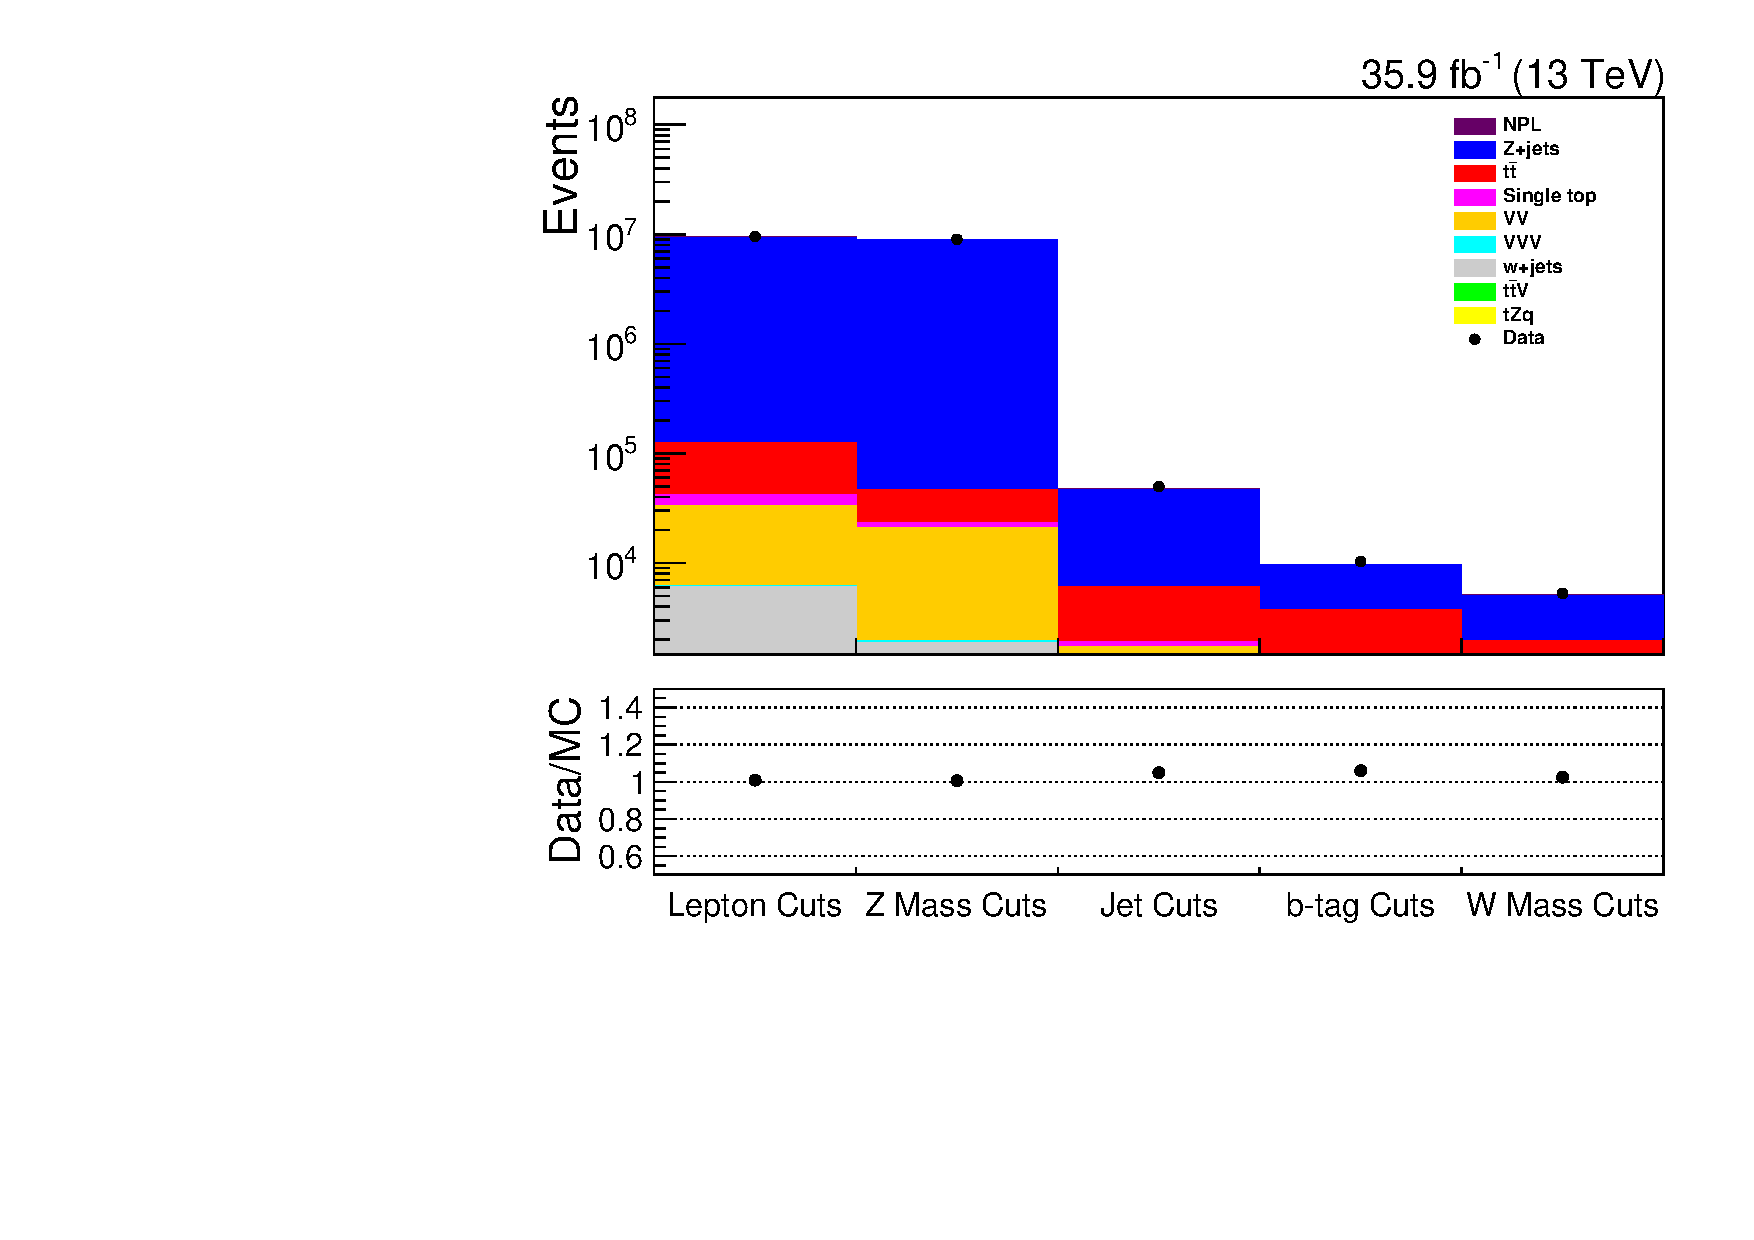
\includegraphics[width=0.83\textwidth]{figs/background-estimation/plots/unblinded/prompt_ee_ttbarInc/cutFlow_log.pdf}
\\
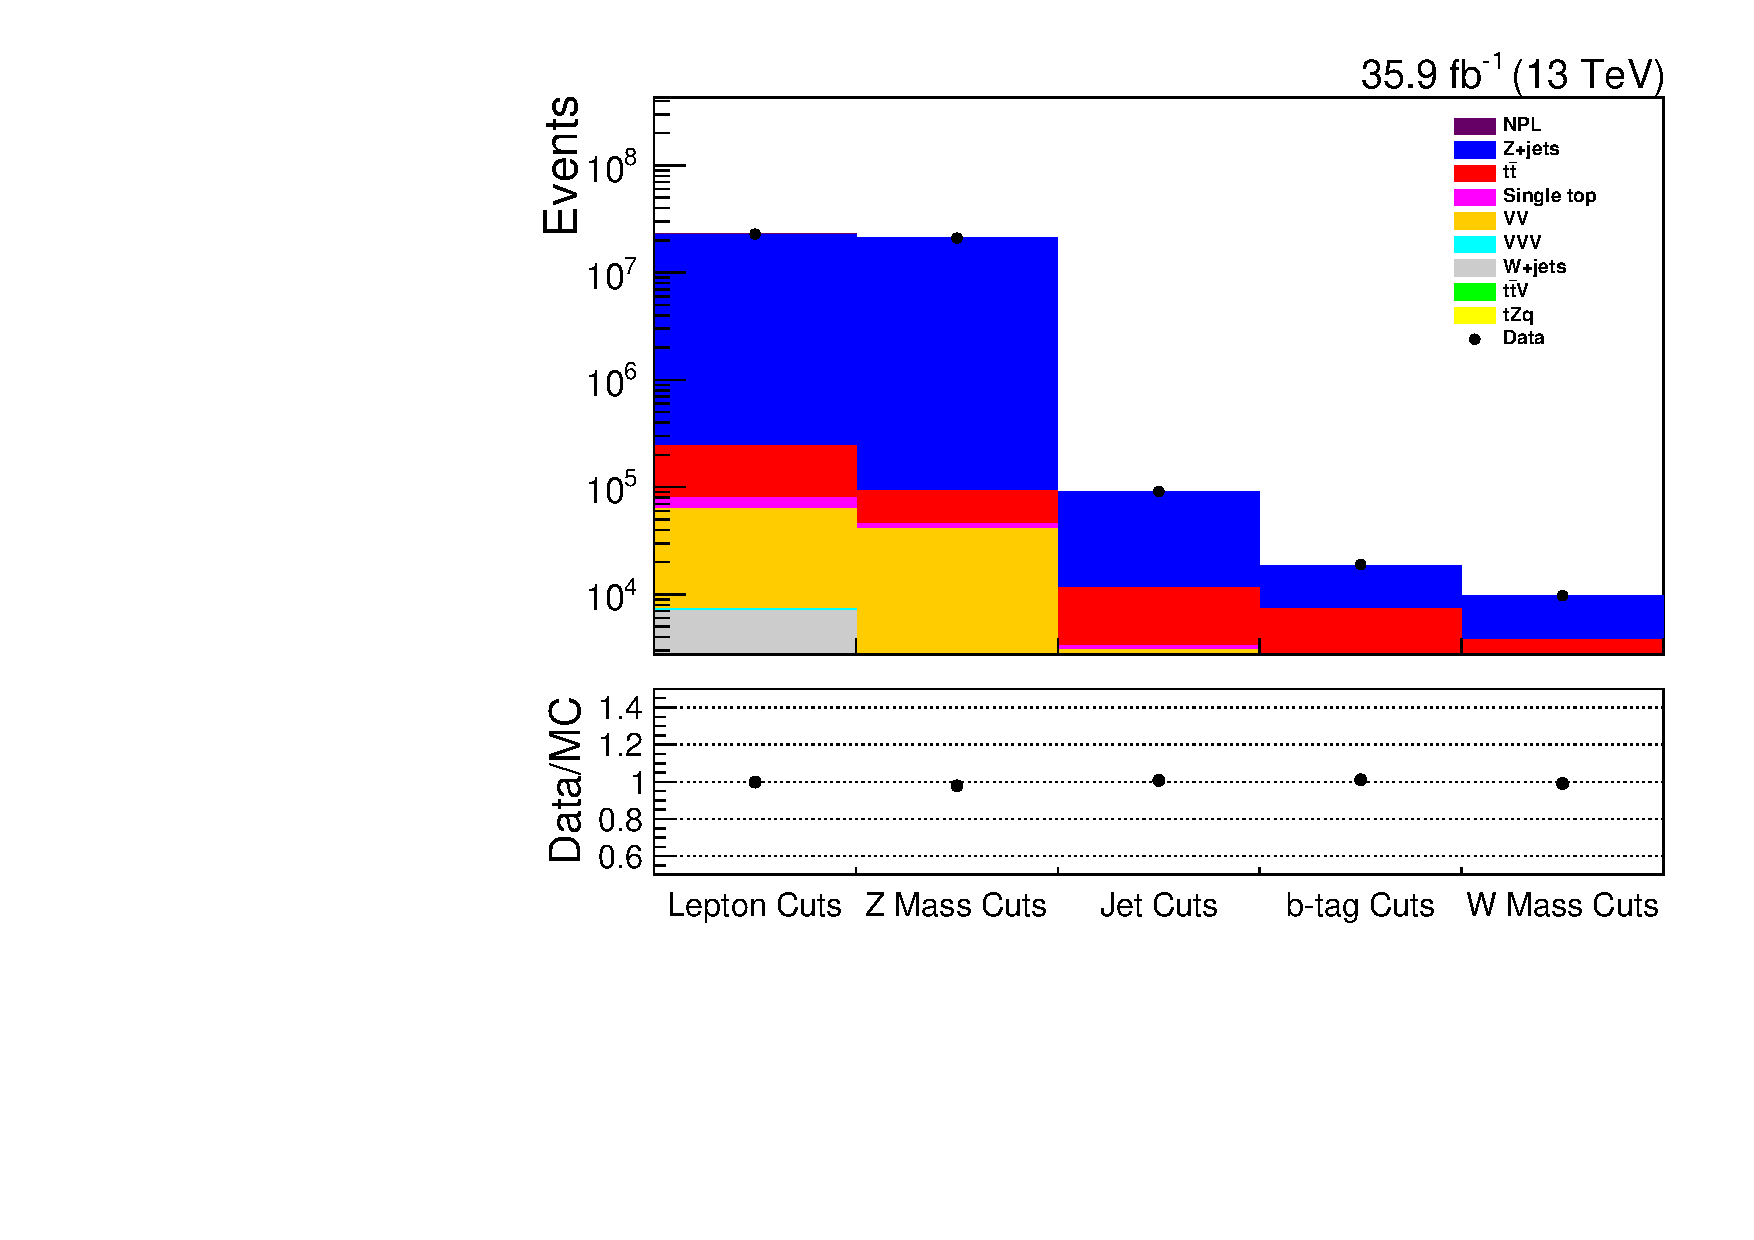
\includegraphics[width=0.83\textwidth]{figs/background-estimation/plots/unblinded/prompt_mumu_ttbarInc/cutFlow_log.pdf}
\caption{
The overall event yield for data and simulation at each stage of applying the signal region selection criteria and simulation corrections for the $ee$ channel (top) and the $\mu\mu$ channel (bottom).
}
\label{fig:SR_cutFlow}
\end{figure}

\begin{figure}[h]
\centering
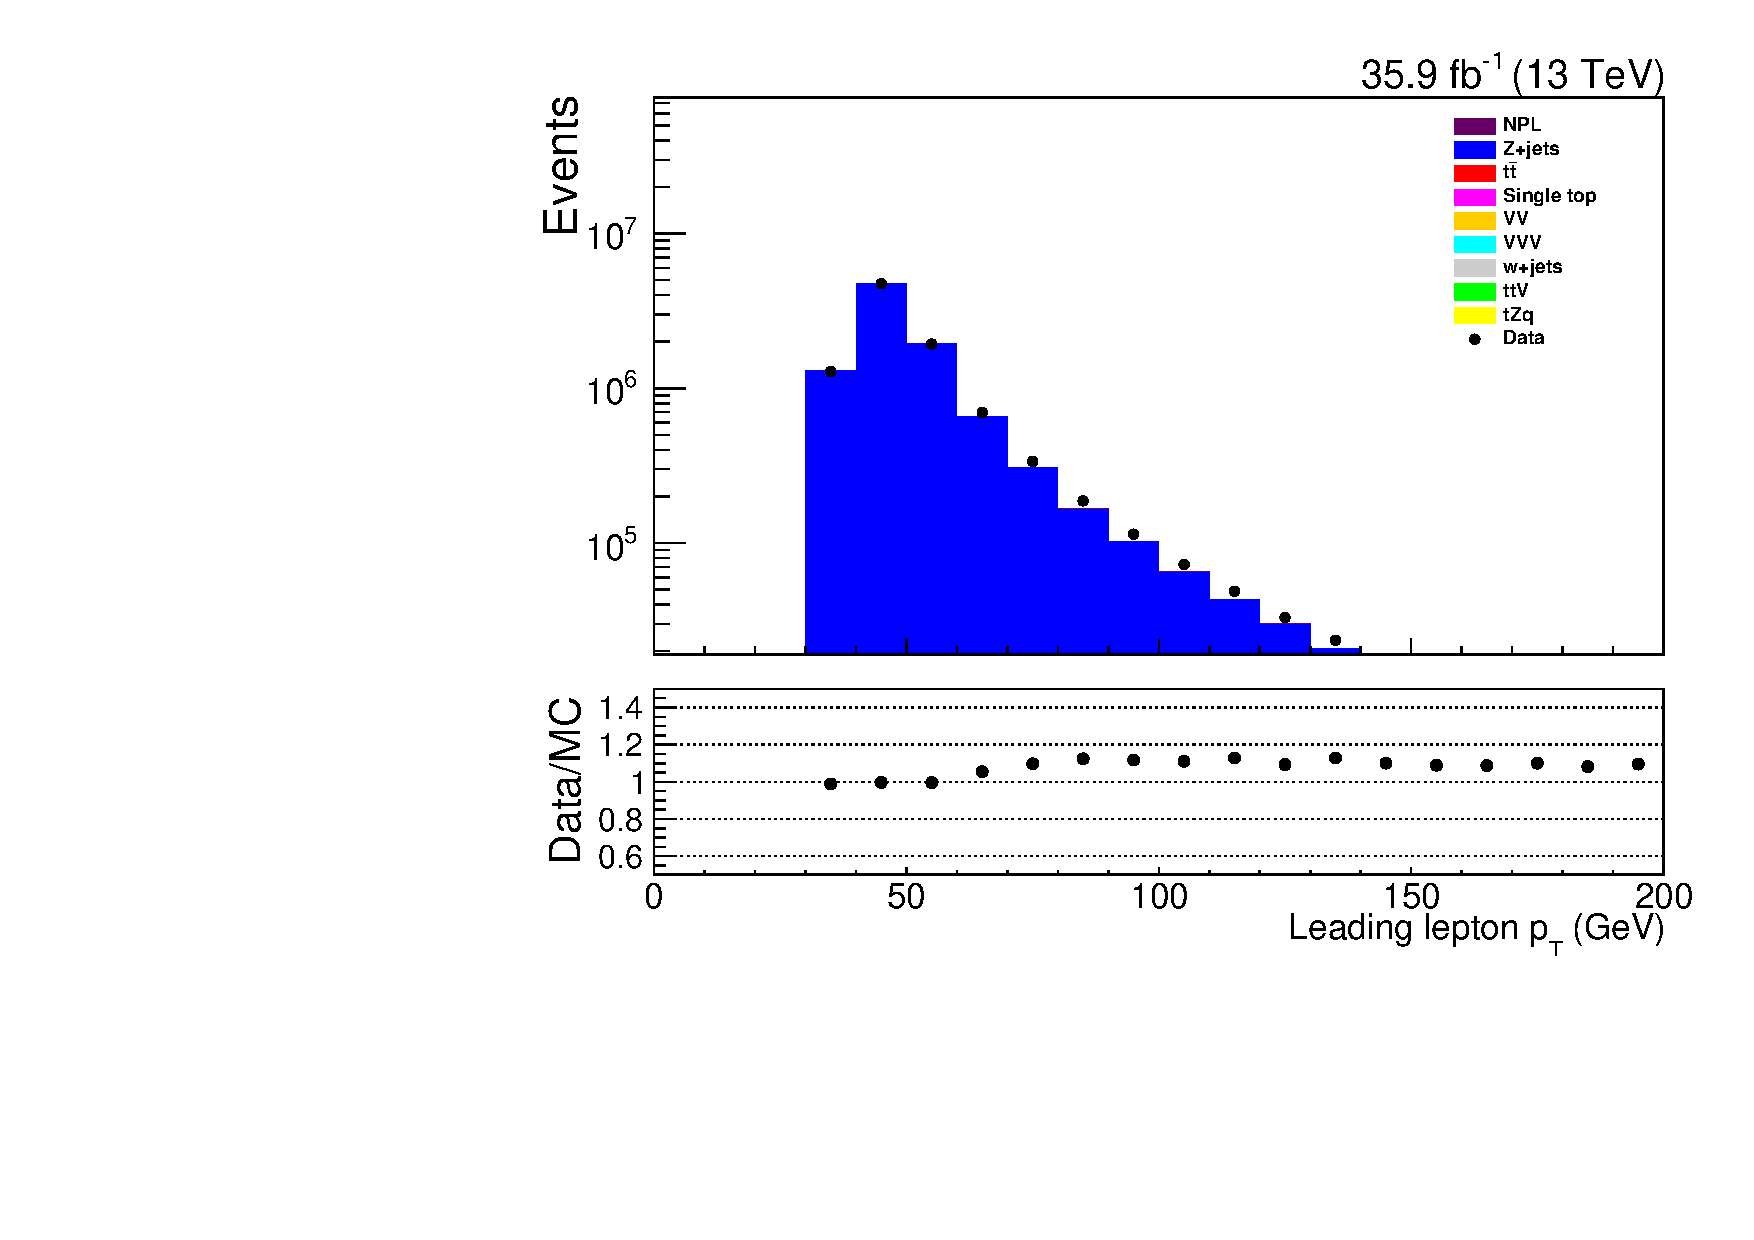
\includegraphics[width=0.47\textwidth]{figs/background-estimation/plots/unblinded/prompt_ee_ttbarInc/lep1Pt_NPL_ee_lepSel_ee_log.pdf}
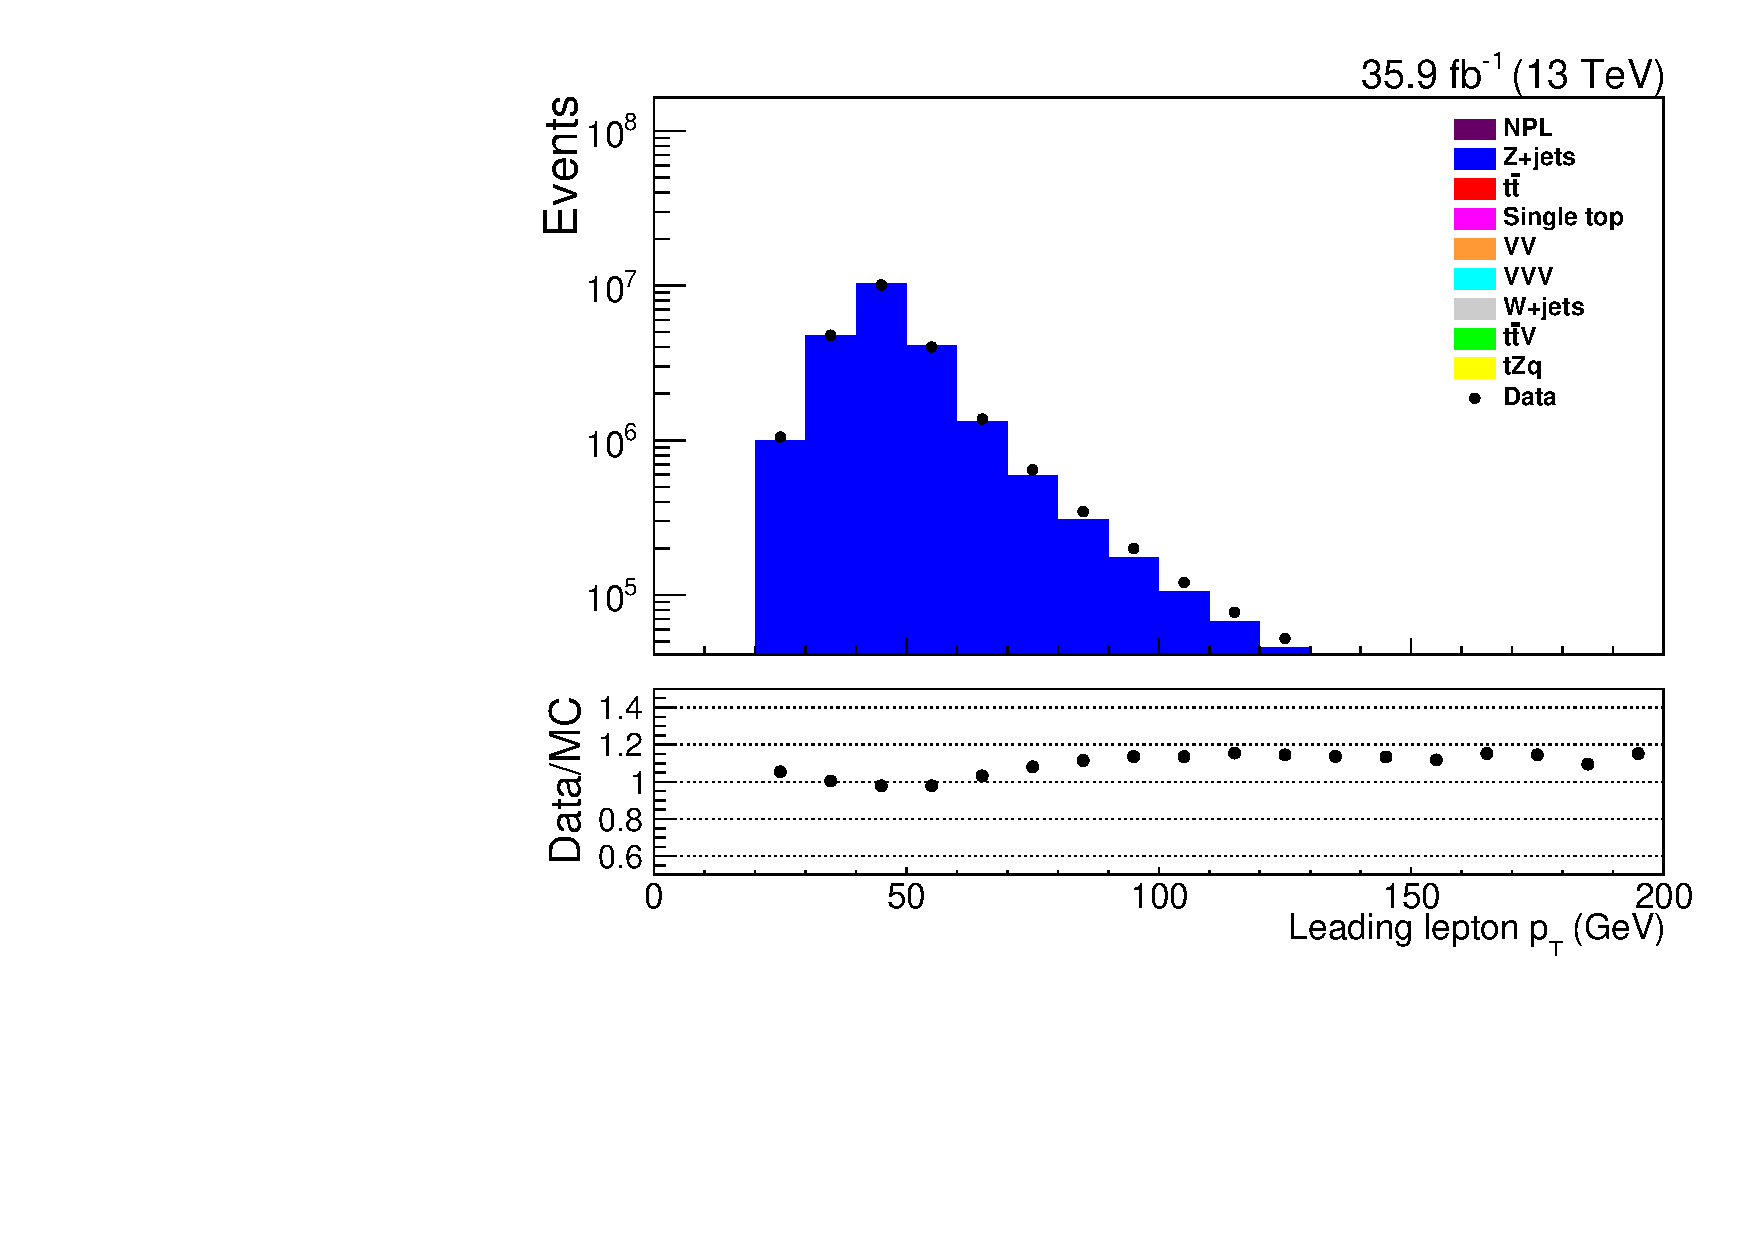
\includegraphics[width=0.47\textwidth]{figs/background-estimation/plots/unblinded/prompt_mumu_ttbarInc/lep1Pt_NPL_mumu_lepSel_mumu_log.pdf}
\\
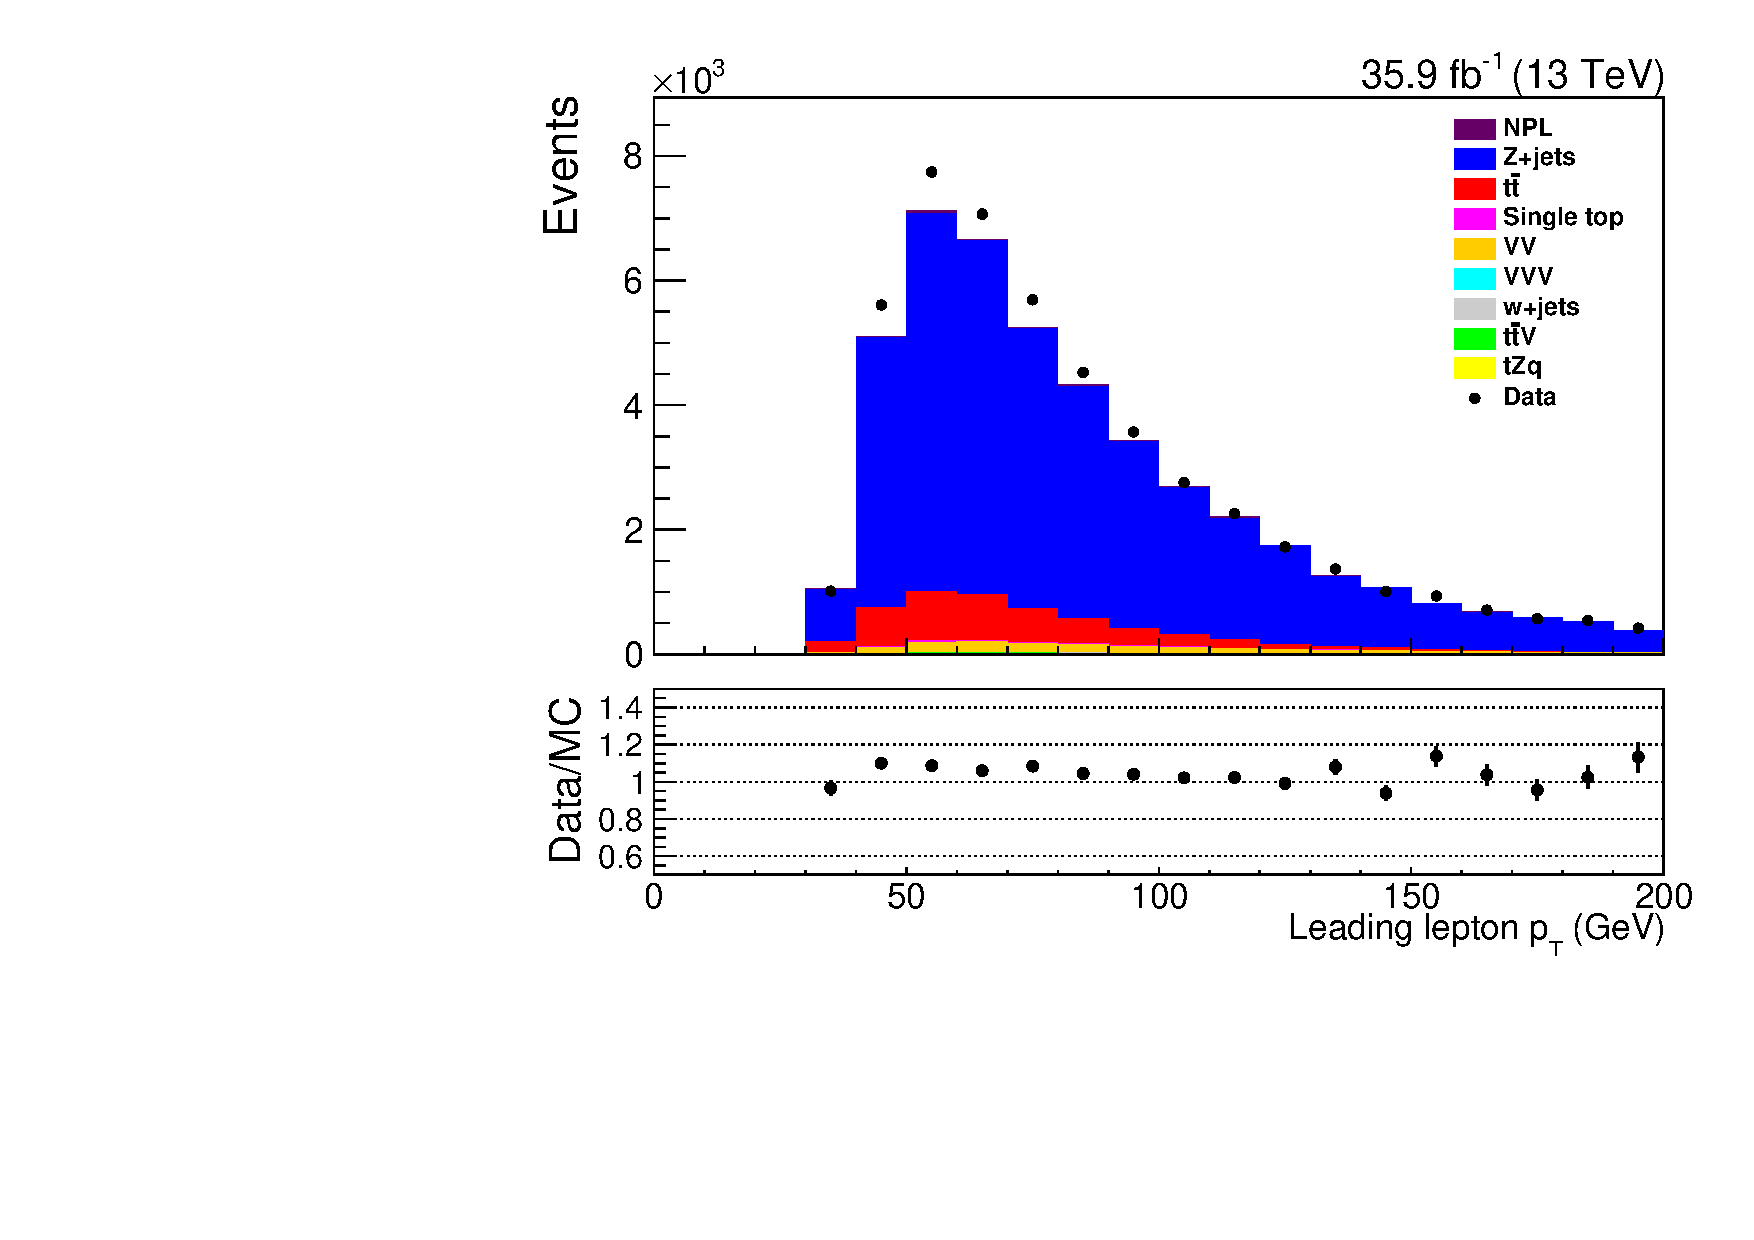
\includegraphics[width=0.47\textwidth]{figs/background-estimation/plots/unblinded/prompt_ee_ttbarInc/lep1Pt_NPL_ee_jetSel_ee.pdf}
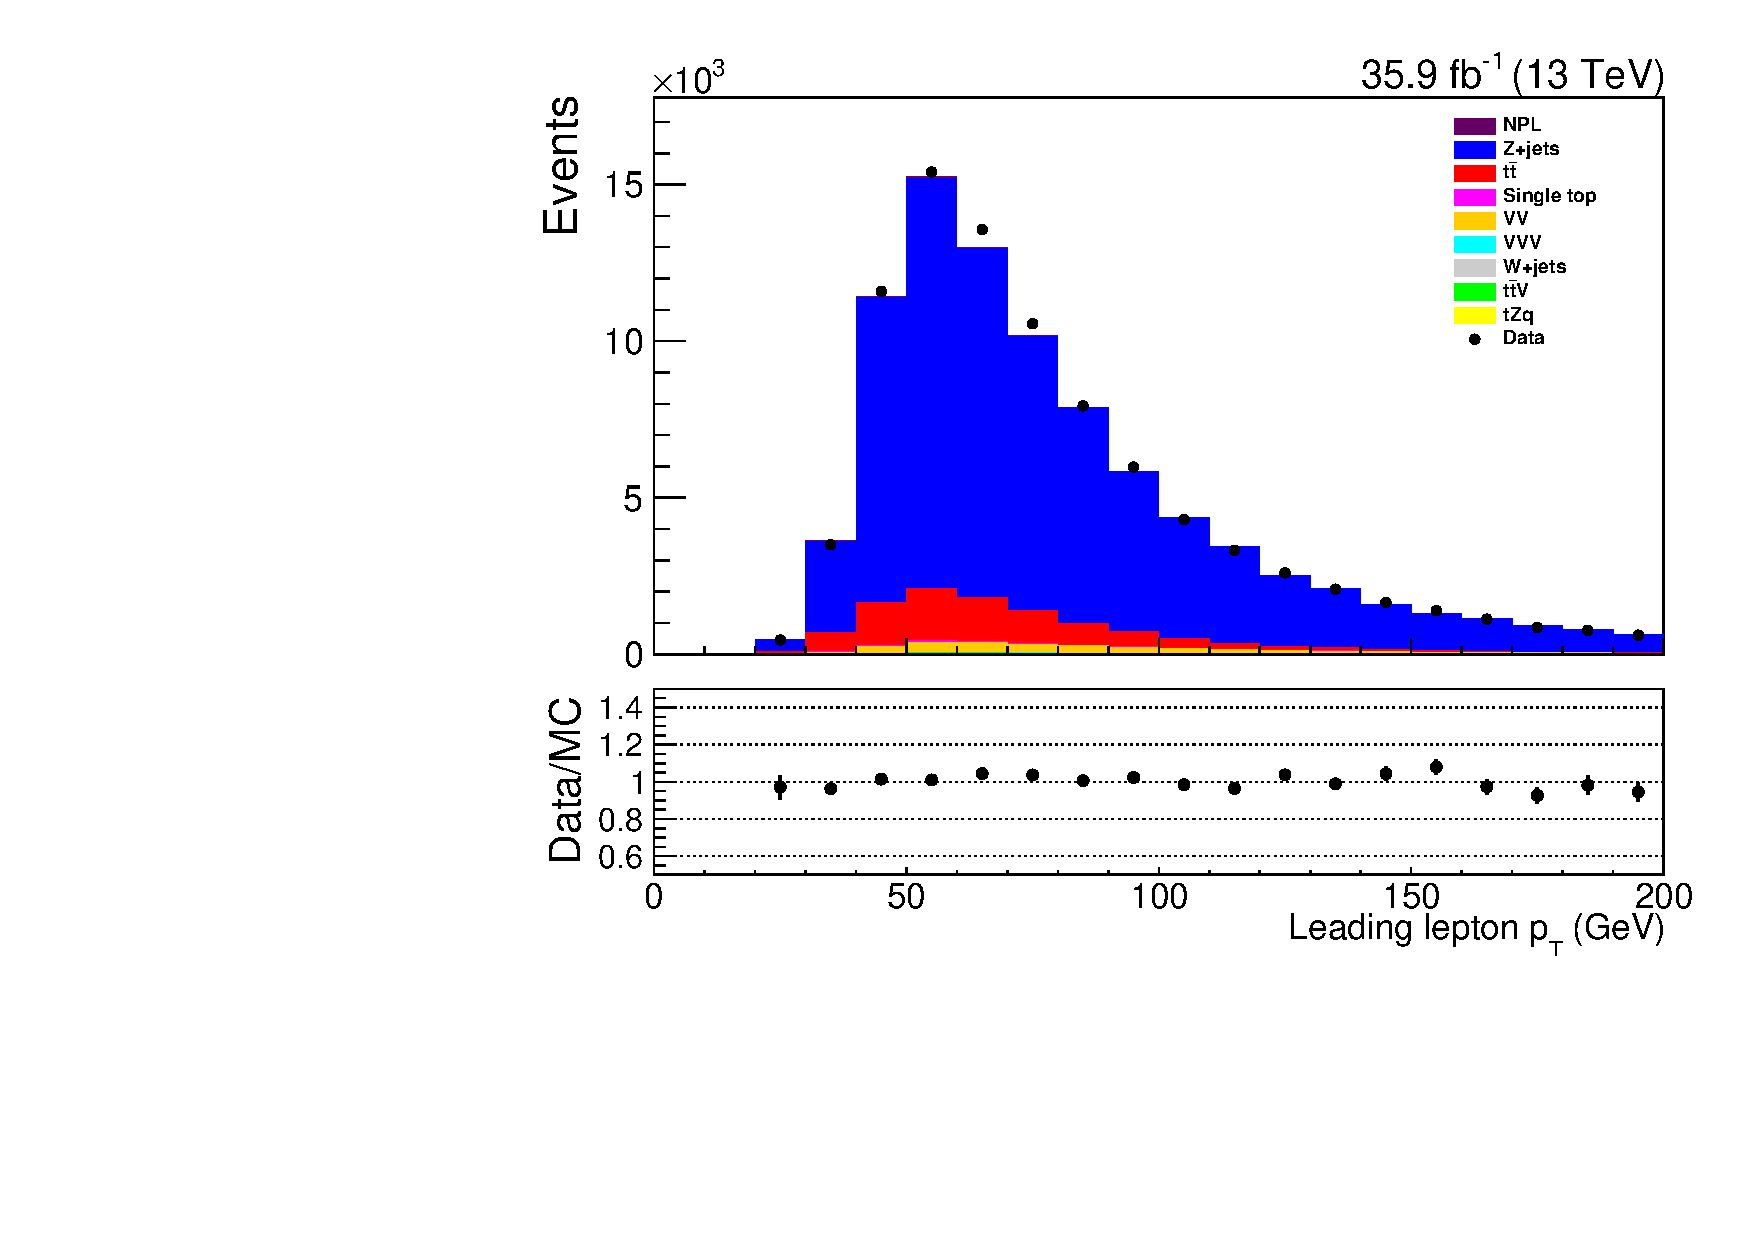
\includegraphics[width=0.47\textwidth]{figs/background-estimation/plots/unblinded/prompt_mumu_ttbarInc/lep1Pt_NPL_mumu_jetSel_mumu.pdf}
\\
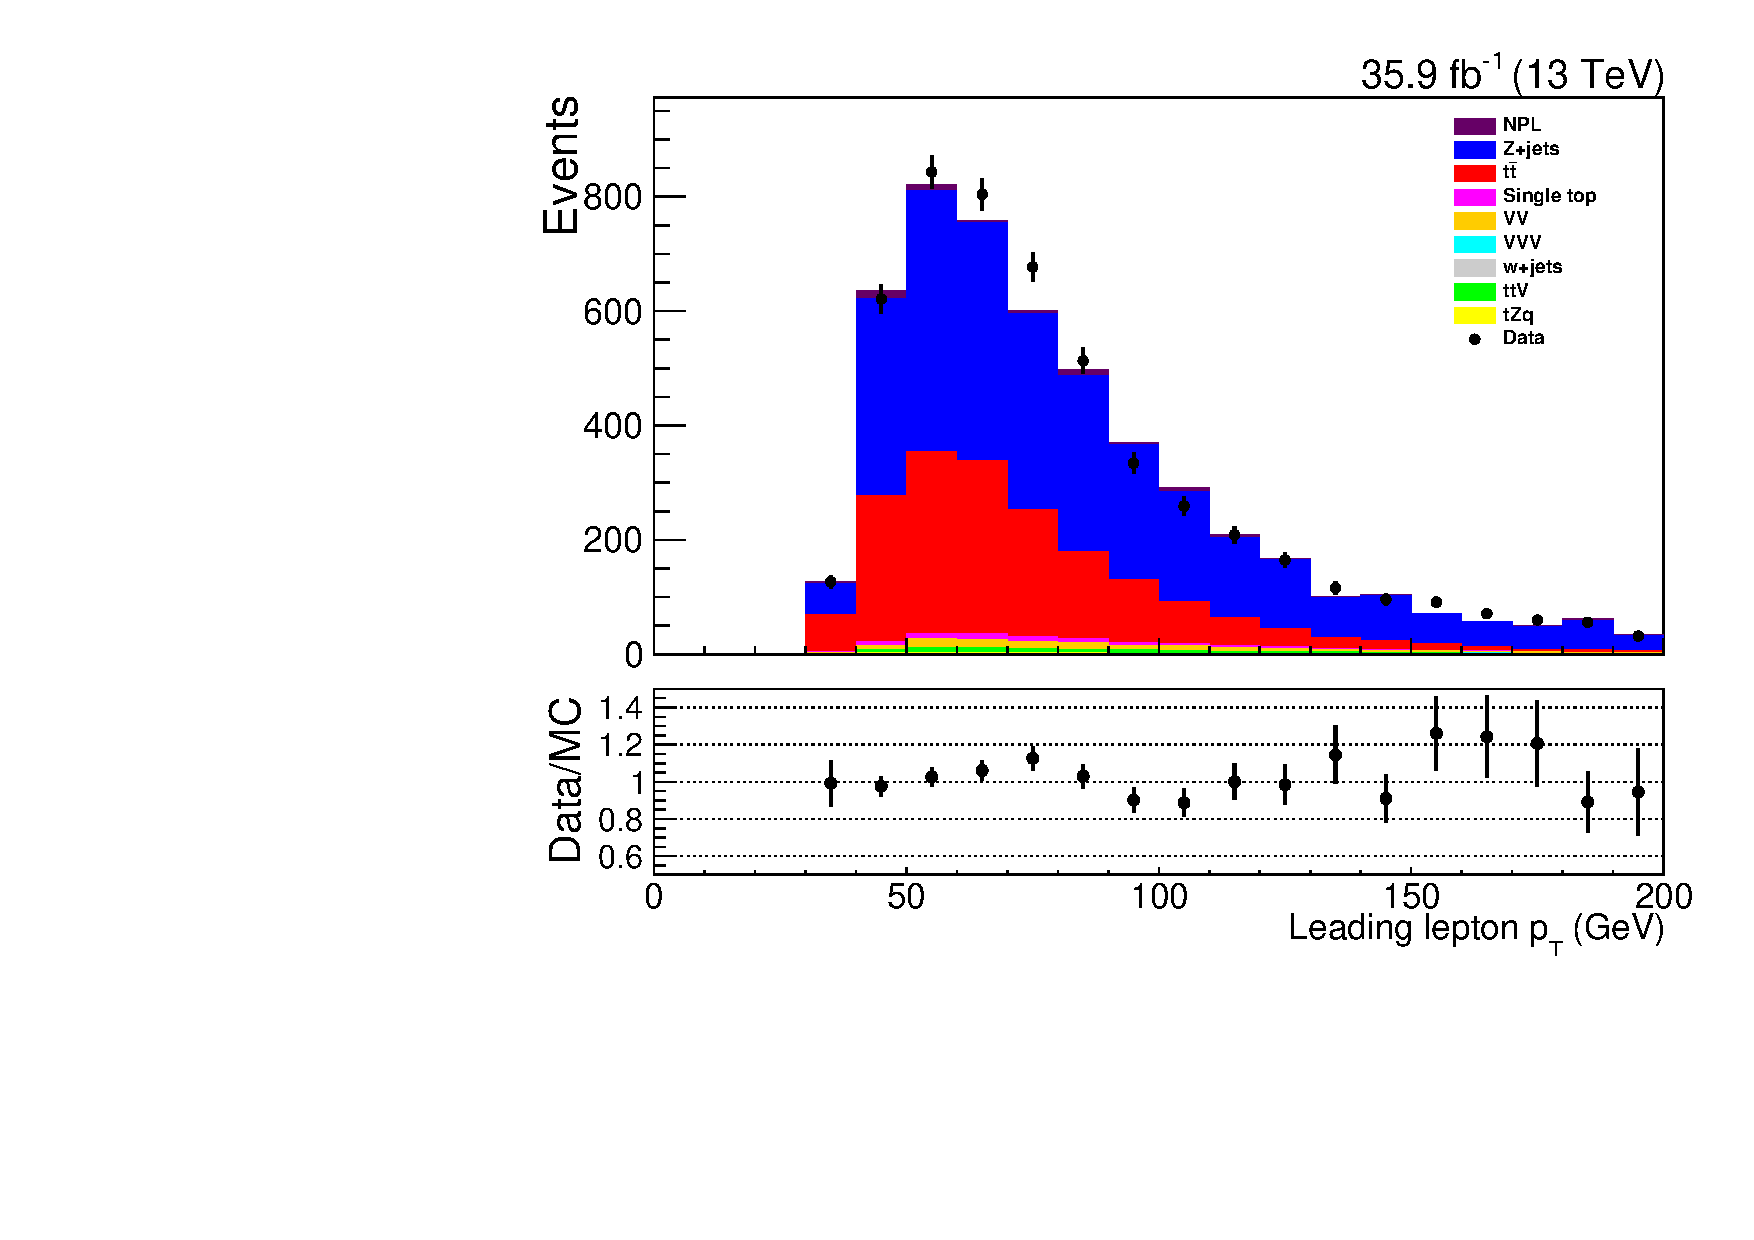
\includegraphics[width=0.47\textwidth]{figs/background-estimation/plots/unblinded/prompt_ee_ttbarInc/lep1Pt_NPL_ee_wMass_ee.pdf}
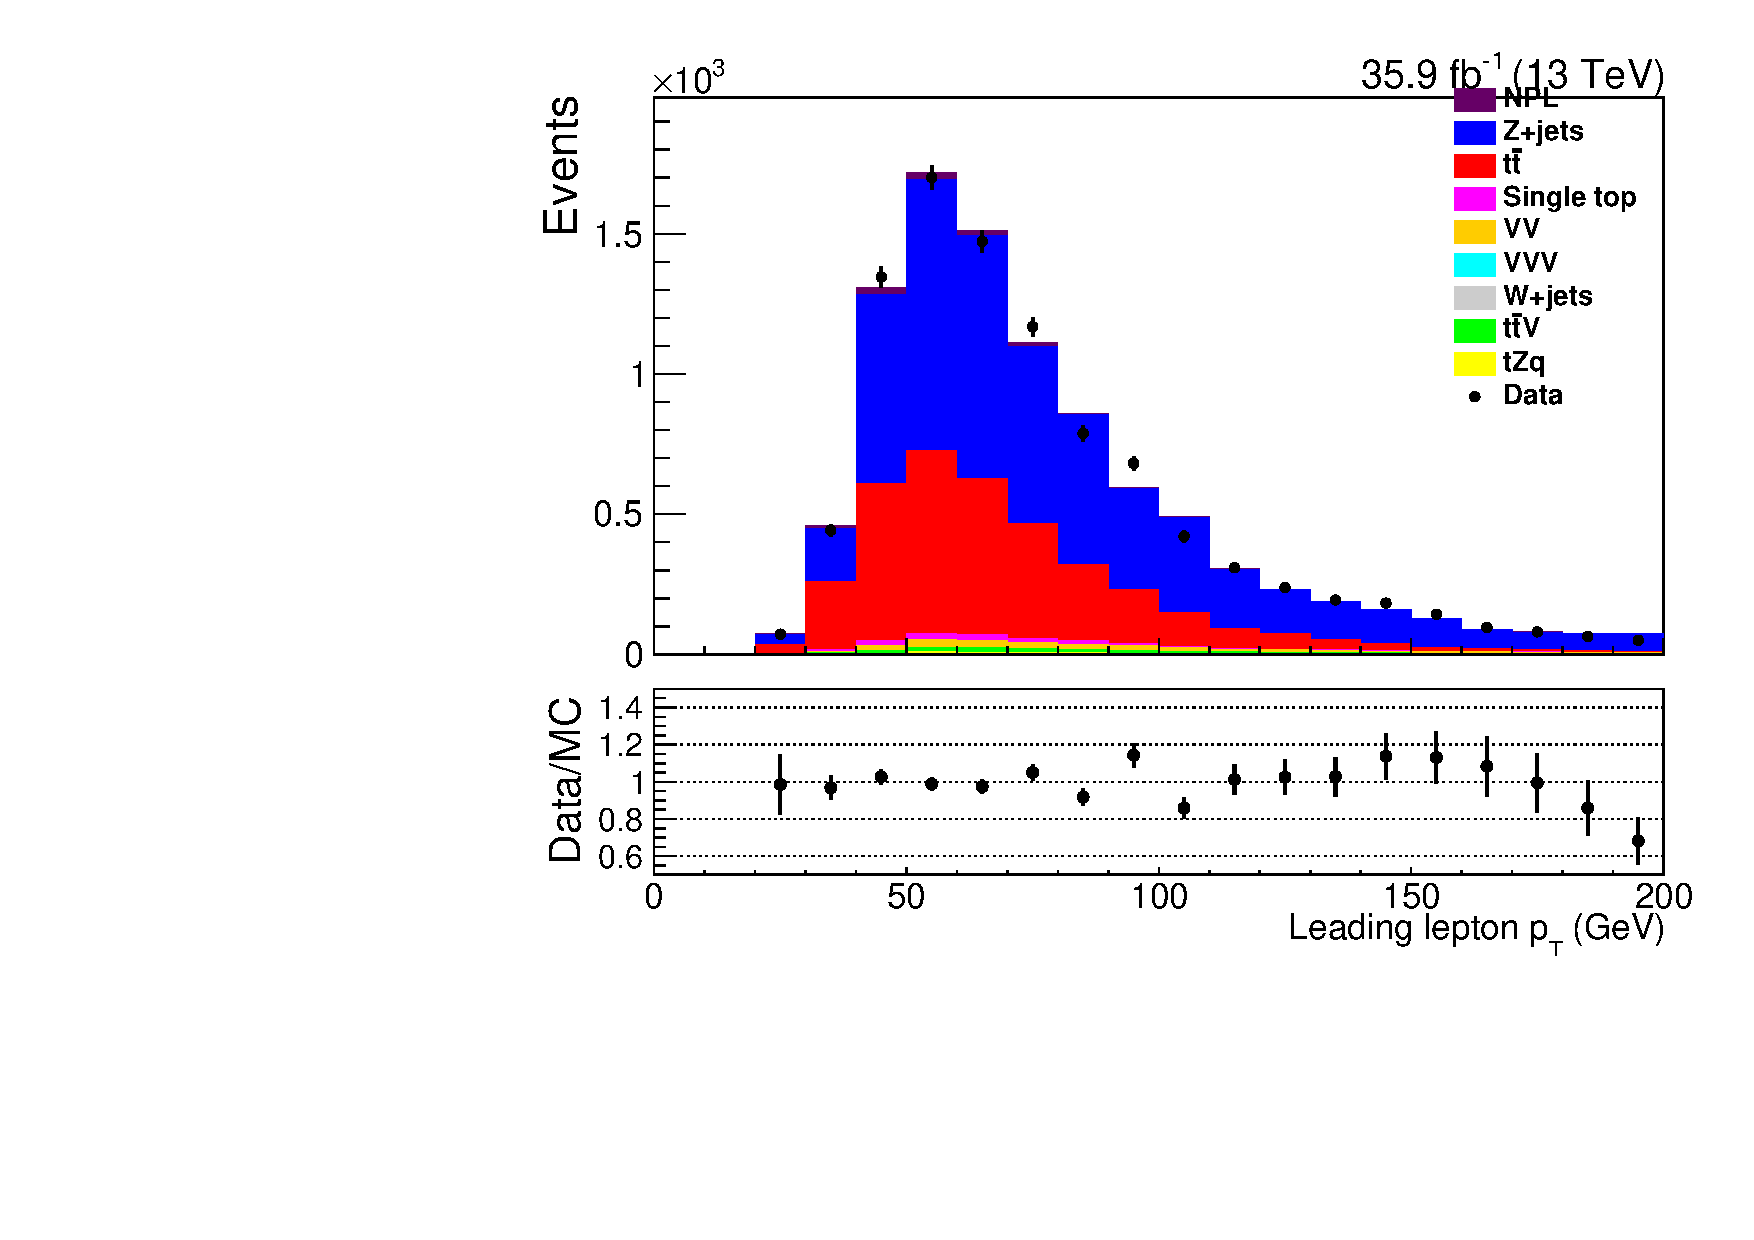
\includegraphics[width=0.47\textwidth]{figs/background-estimation/plots/unblinded/prompt_mumu_ttbarInc/lep1Pt_NPL_mumu_wMass_mumu.pdf}
\caption{
The leading lepton \pT following only the lepton selection criteria and simulation corrections (top), the jet selection criteria (middle) and all of the signal region selection criteria (bottom).
}
\label{fig:SR_lep1Pt}
\end{figure}

\begin{figure}[h]
\centering
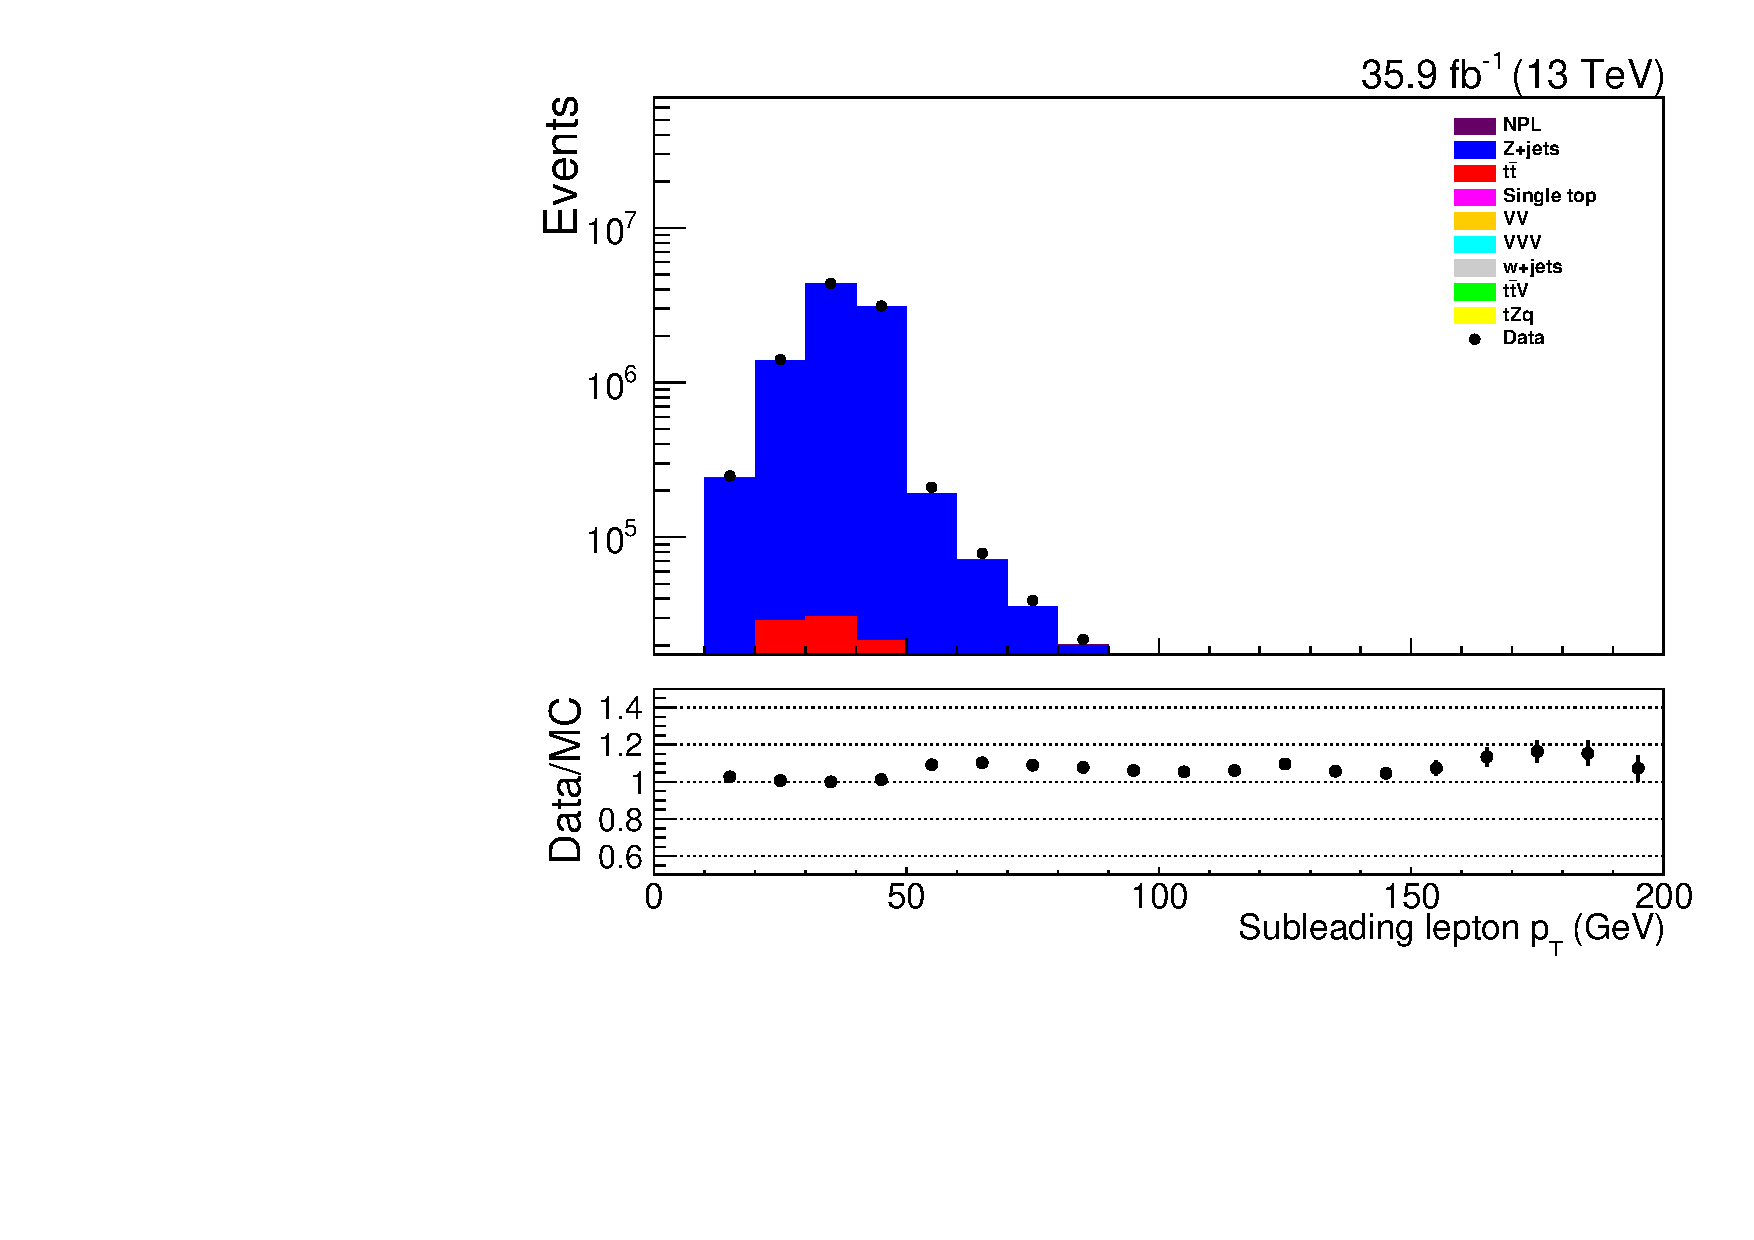
\includegraphics[width=0.47\textwidth]{figs/background-estimation/plots/unblinded/prompt_ee_ttbarInc/lep2Pt_NPL_ee_lepSel_ee_log.pdf}
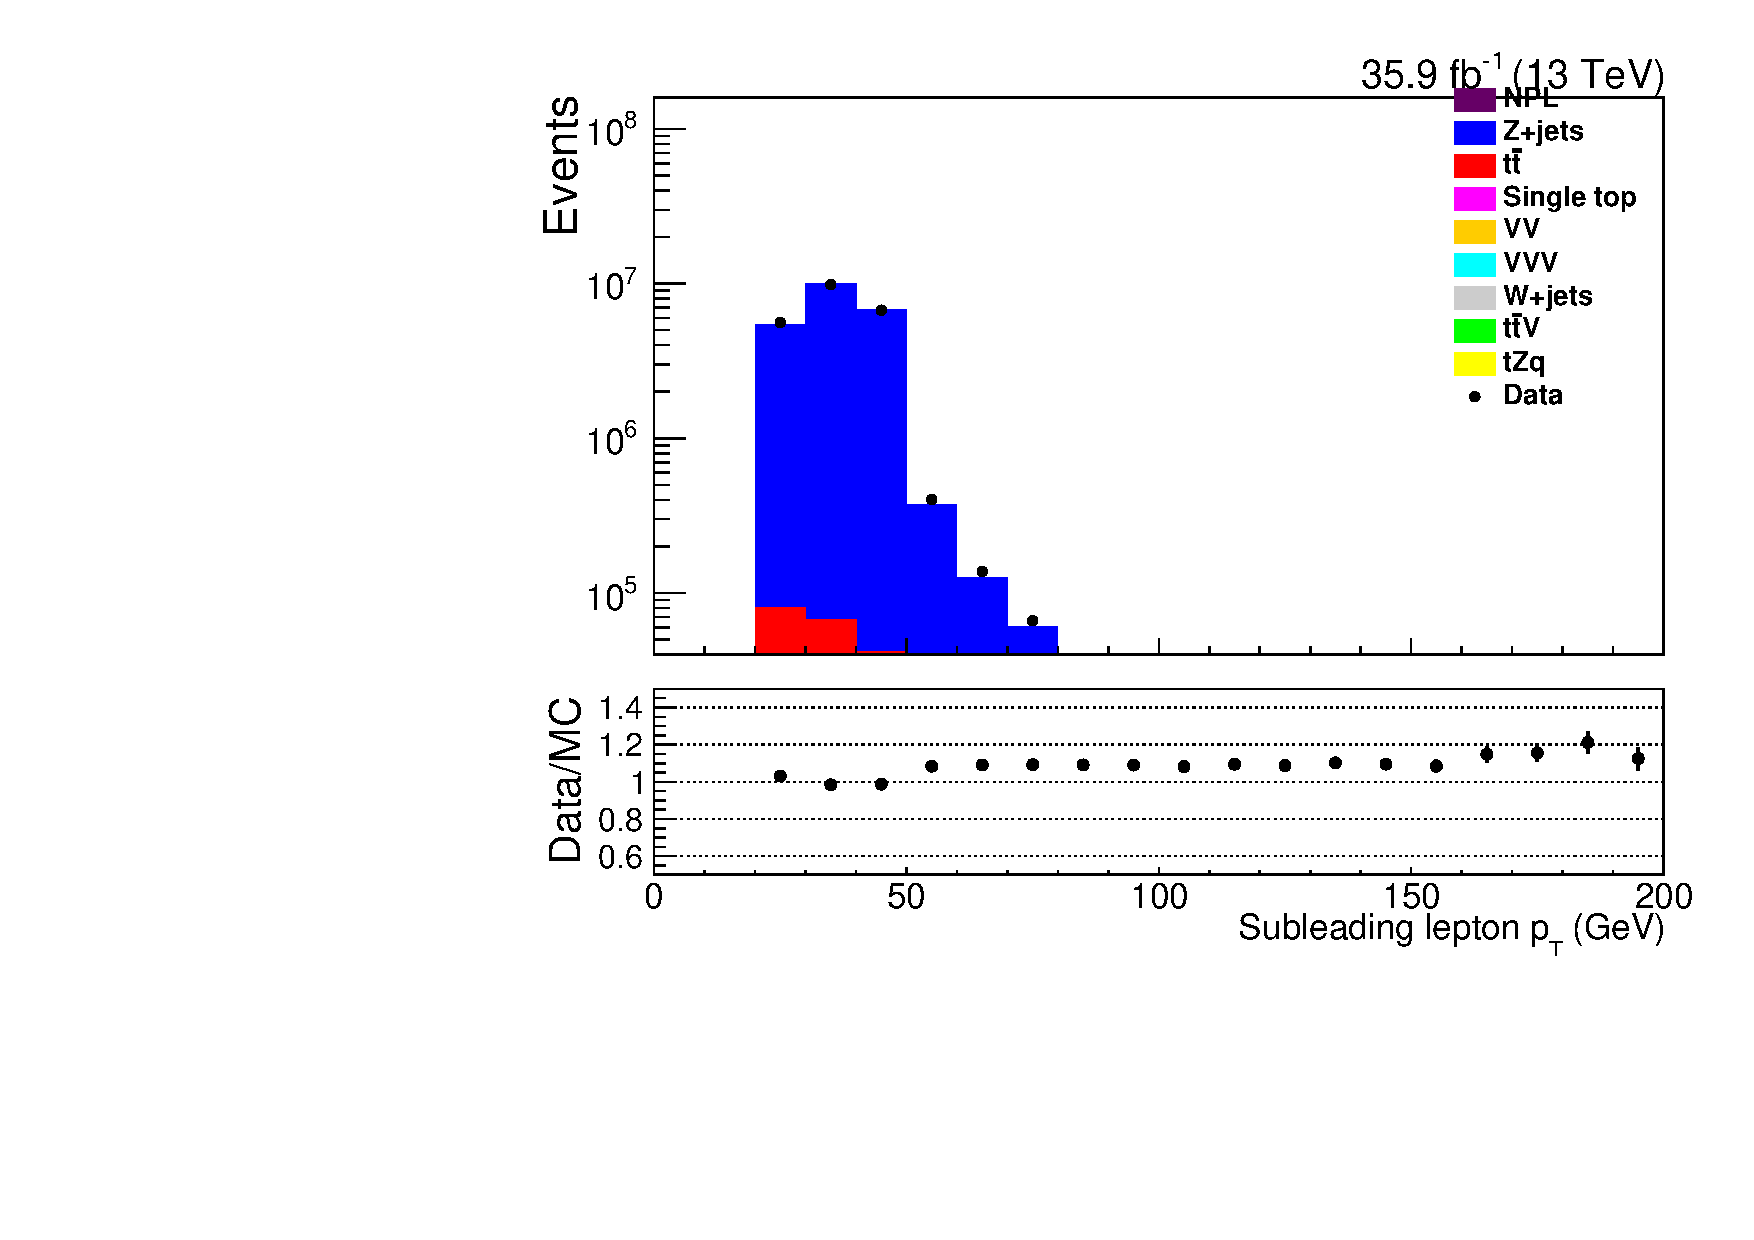
\includegraphics[width=0.47\textwidth]{figs/background-estimation/plots/unblinded/prompt_mumu_ttbarInc/lep2Pt_NPL_mumu_lepSel_mumu_log.pdf}
\\
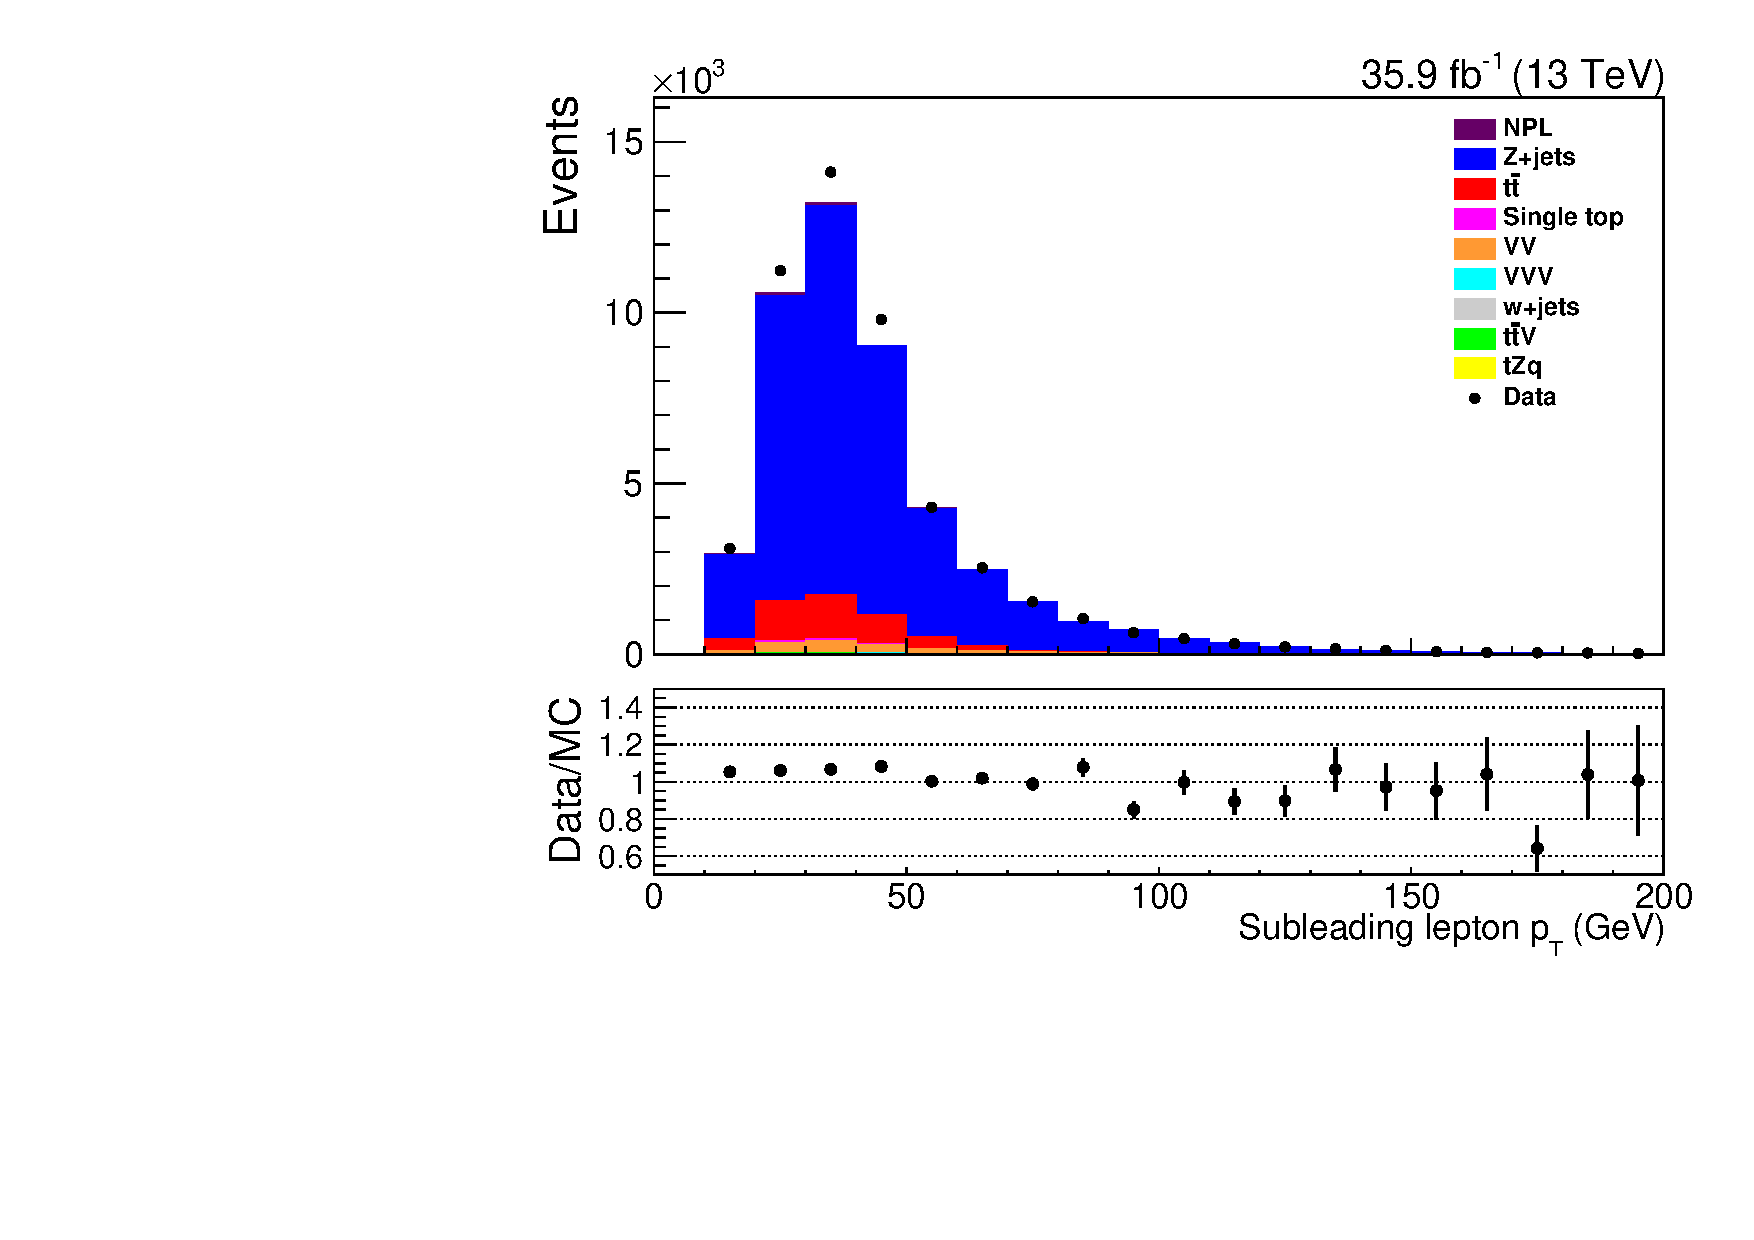
\includegraphics[width=0.47\textwidth]{figs/background-estimation/plots/unblinded/prompt_ee_ttbarInc/lep2Pt_NPL_ee_jetSel_ee.pdf}
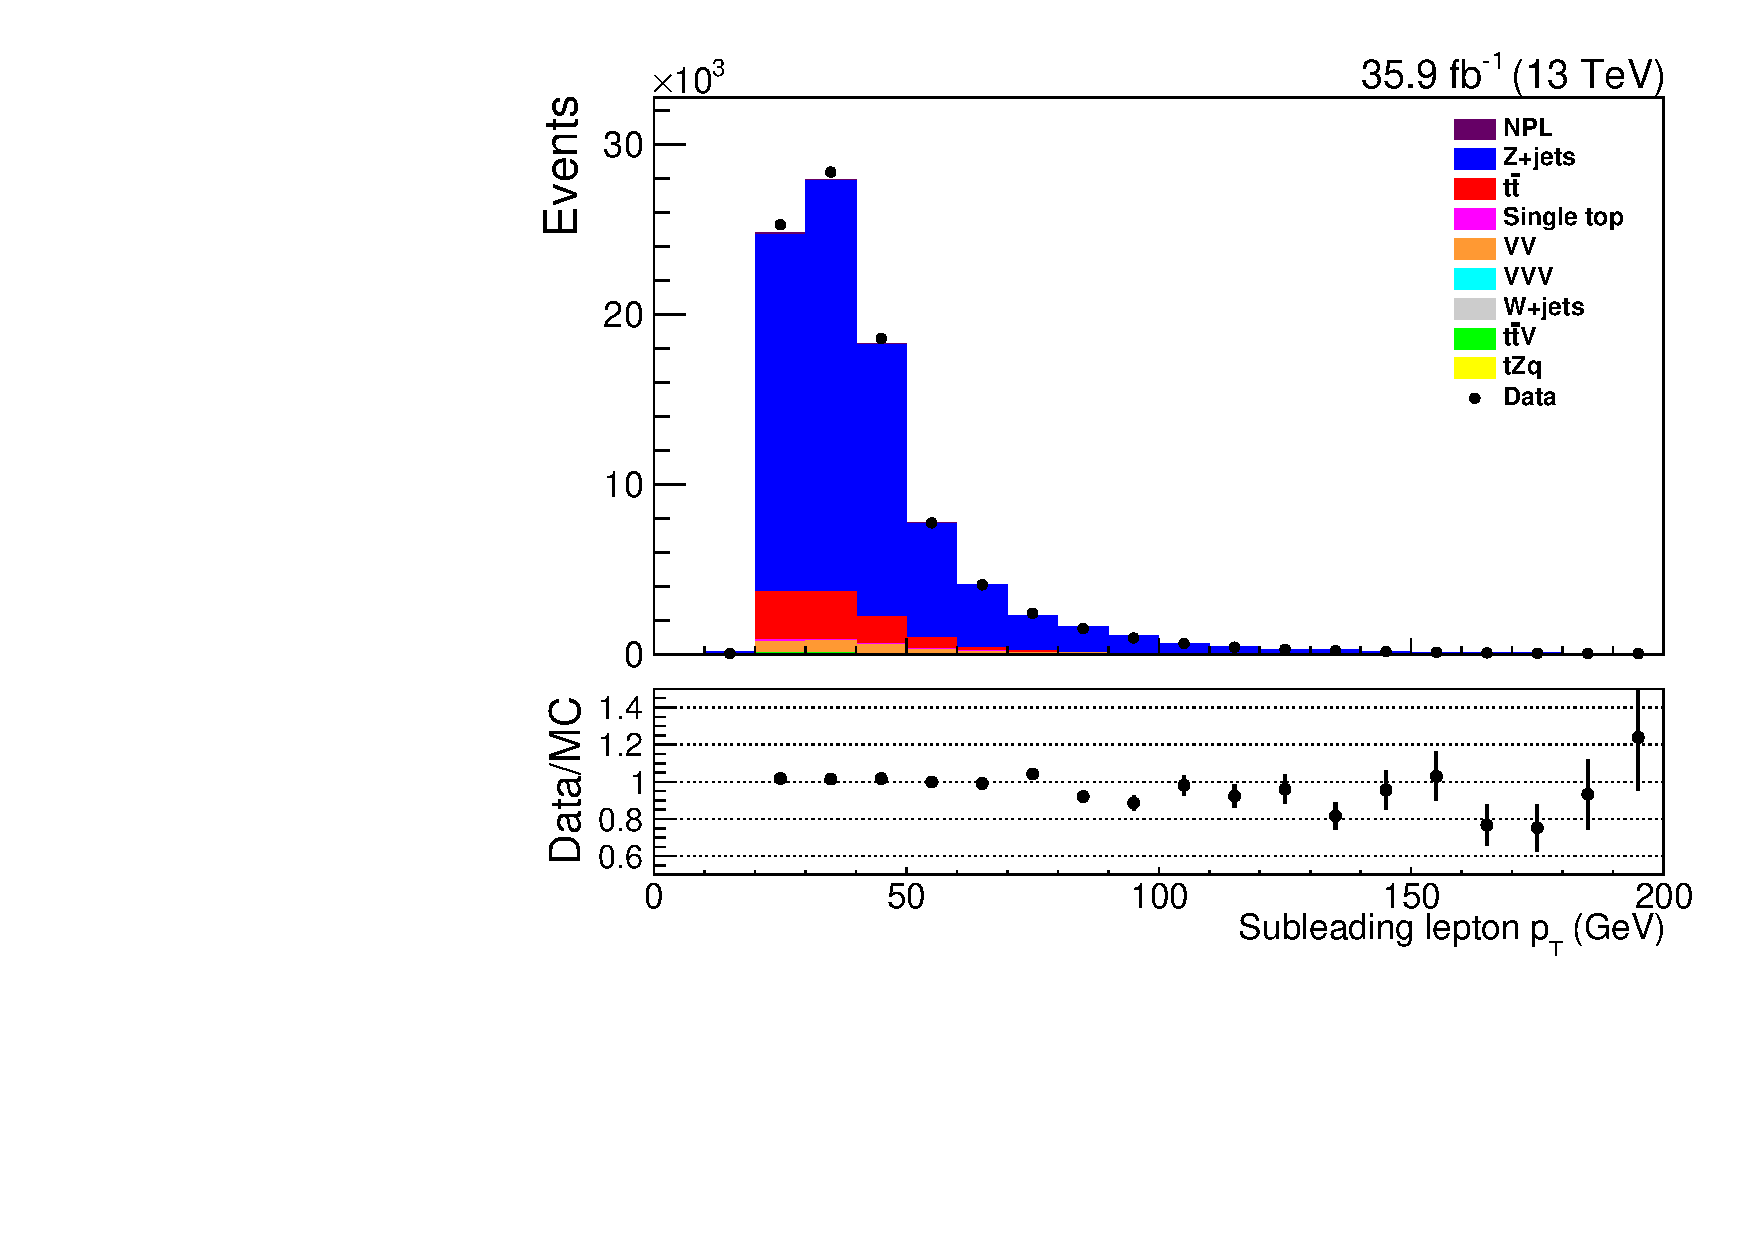
\includegraphics[width=0.47\textwidth]{figs/background-estimation/plots/unblinded/prompt_mumu_ttbarInc/lep2Pt_NPL_mumu_jetSel_mumu.pdf}
\\
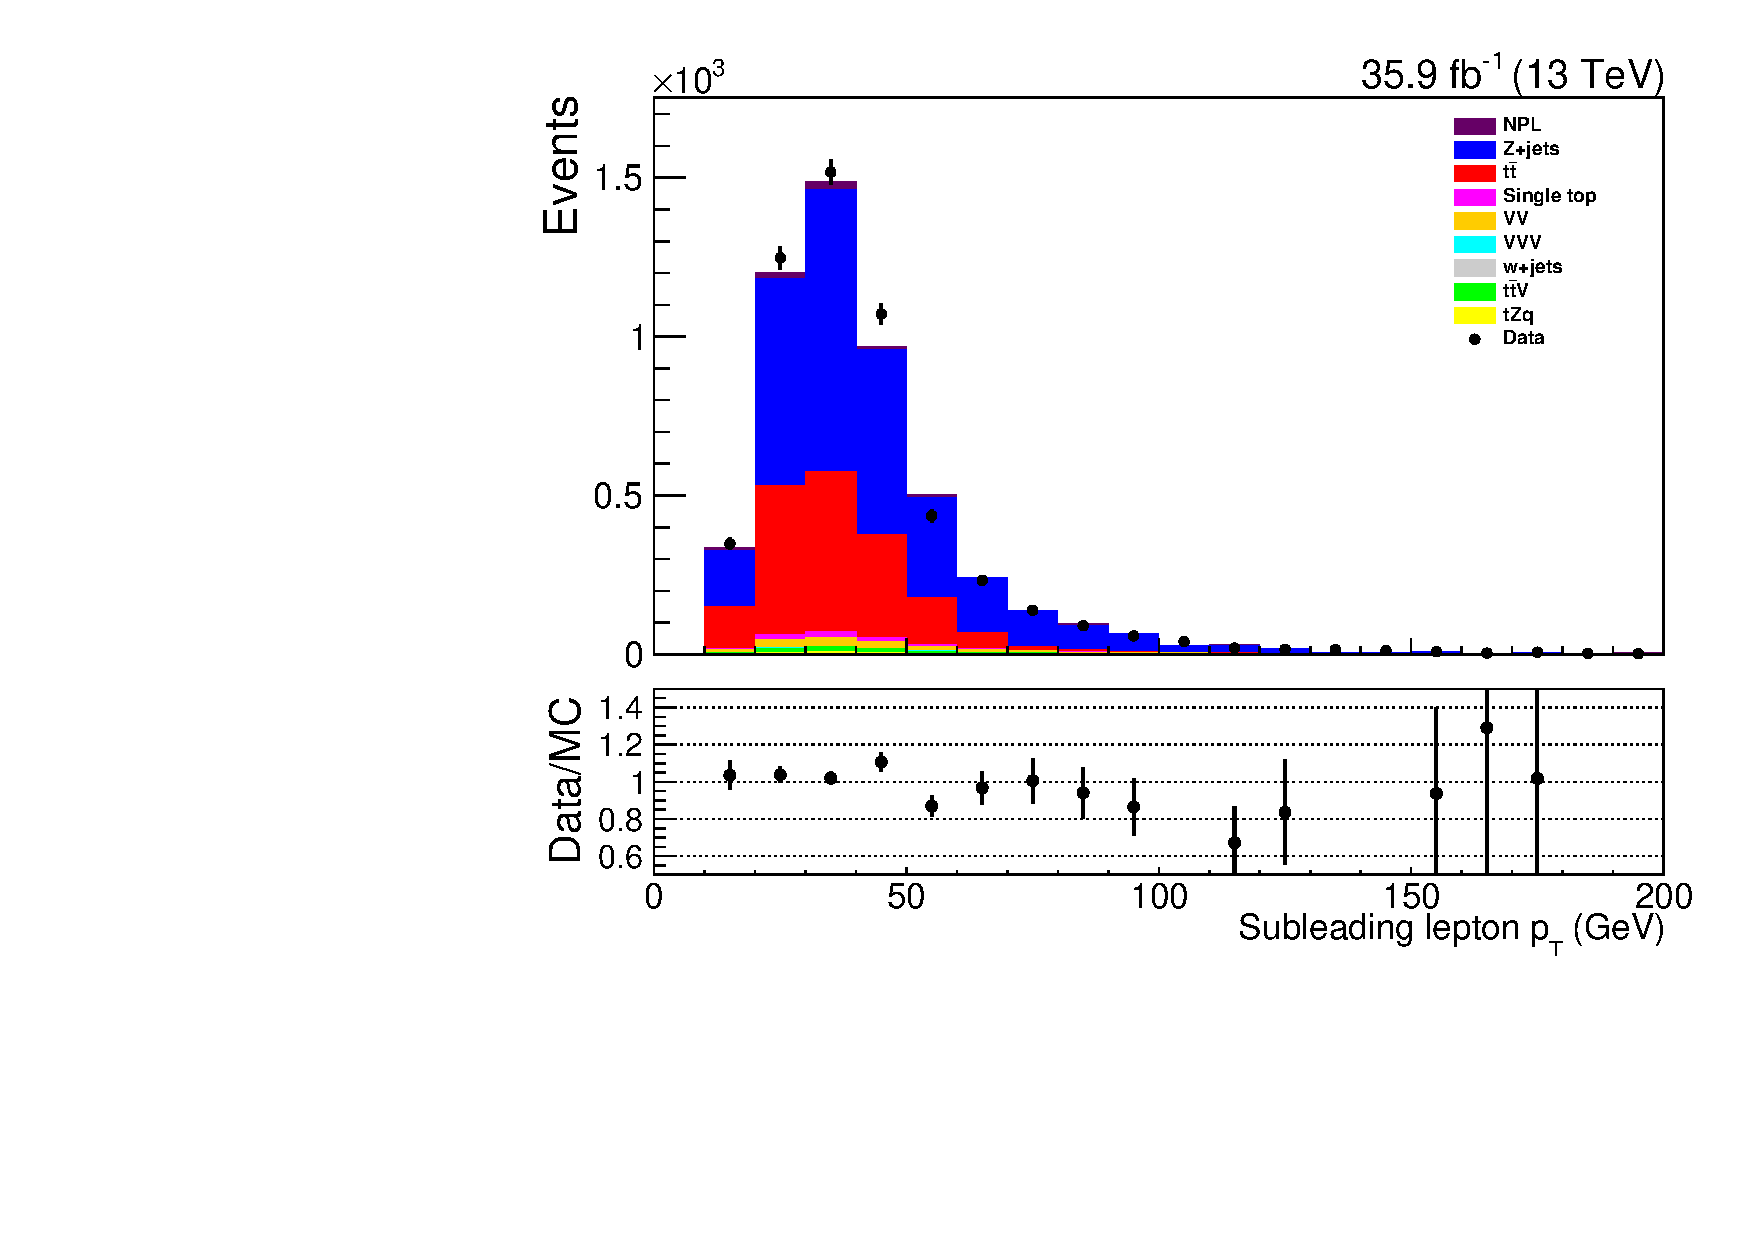
\includegraphics[width=0.47\textwidth]{figs/background-estimation/plots/unblinded/prompt_ee_ttbarInc/lep2Pt_NPL_ee_wMass_ee.pdf}
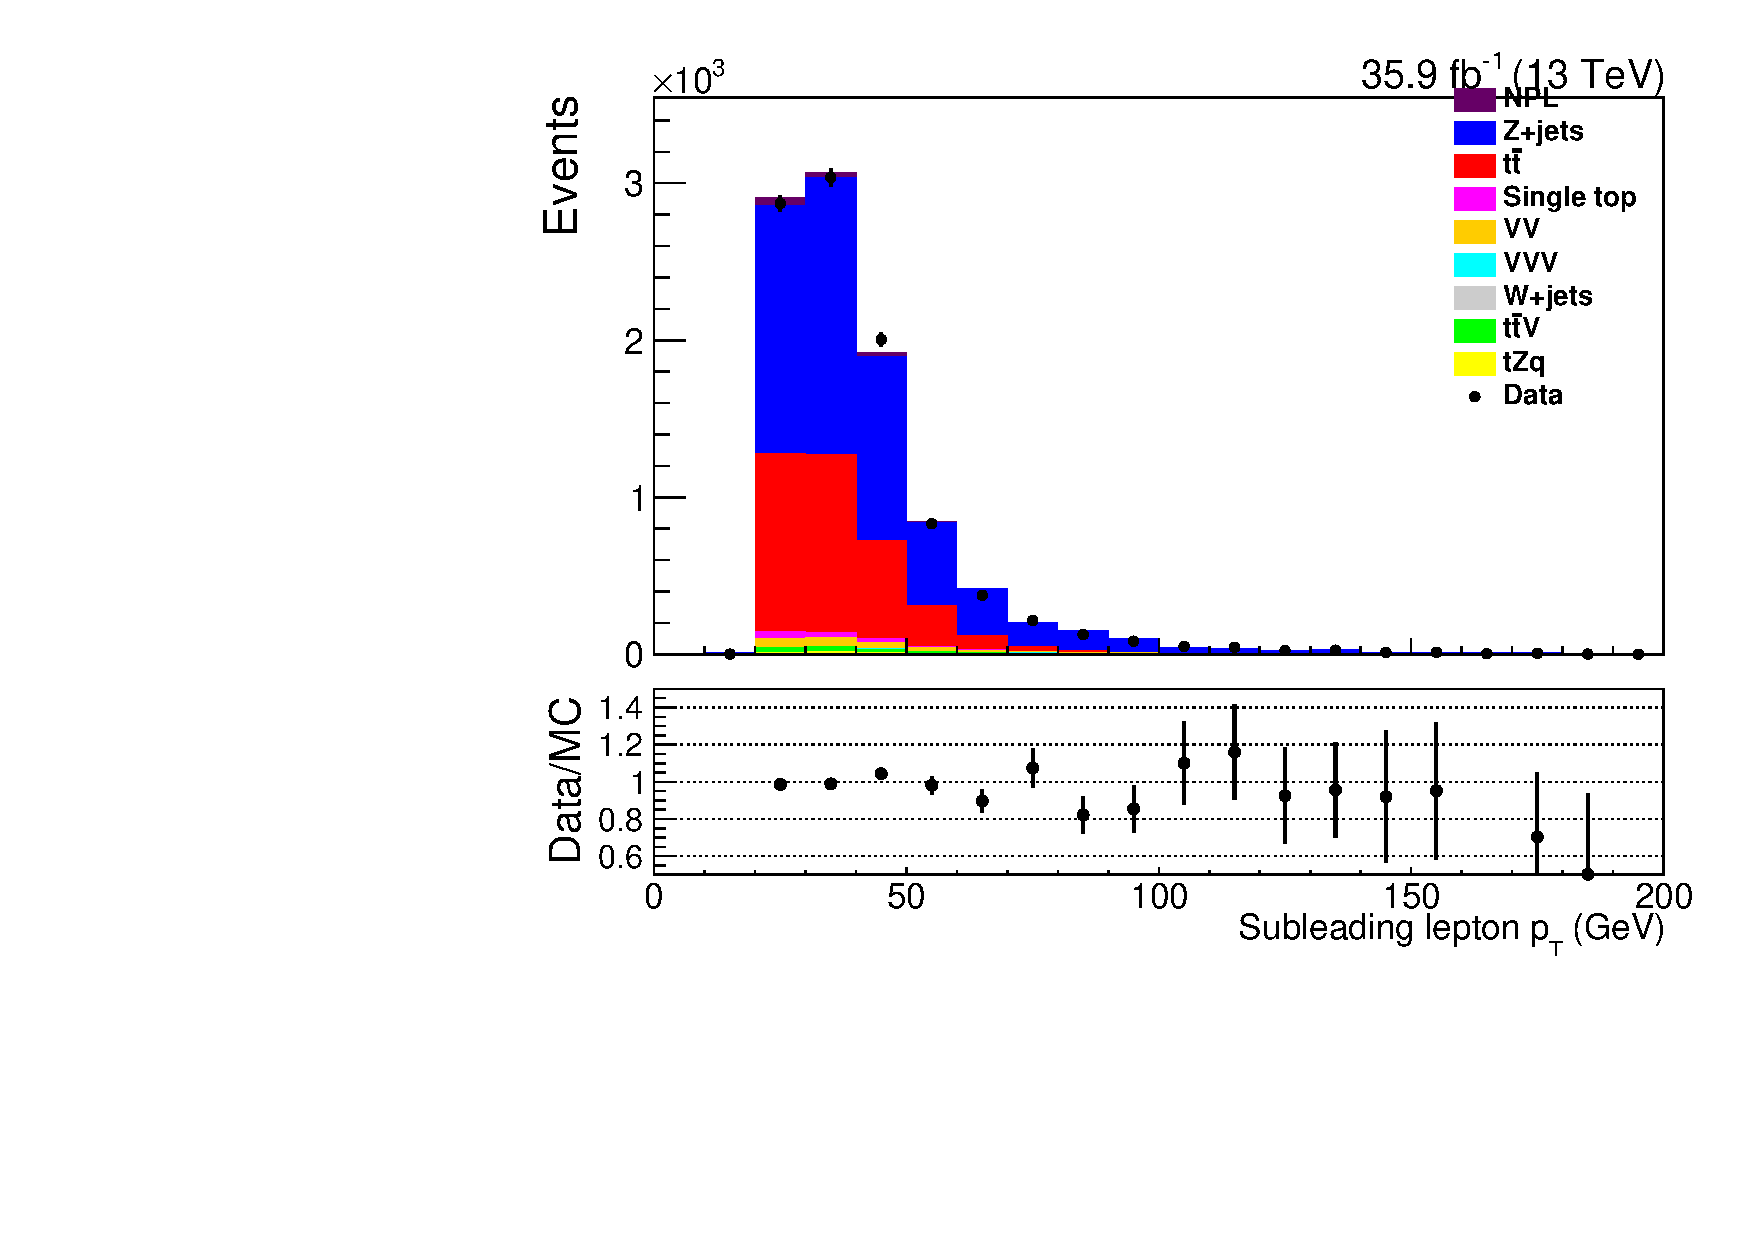
\includegraphics[width=0.47\textwidth]{figs/background-estimation/plots/unblinded/prompt_mumu_ttbarInc/lep2Pt_NPL_mumu_wMass_mumu.pdf}
\caption{
The subleading lepton \pT following only the lepton selection criteria and simulation corrections (top), the jet selection criteria (middle) and all of the signal region selection criteria (bottom).
}
\label{fig:SR_lep2Pt}
\end{figure}

\begin{figure}[h]
\centering
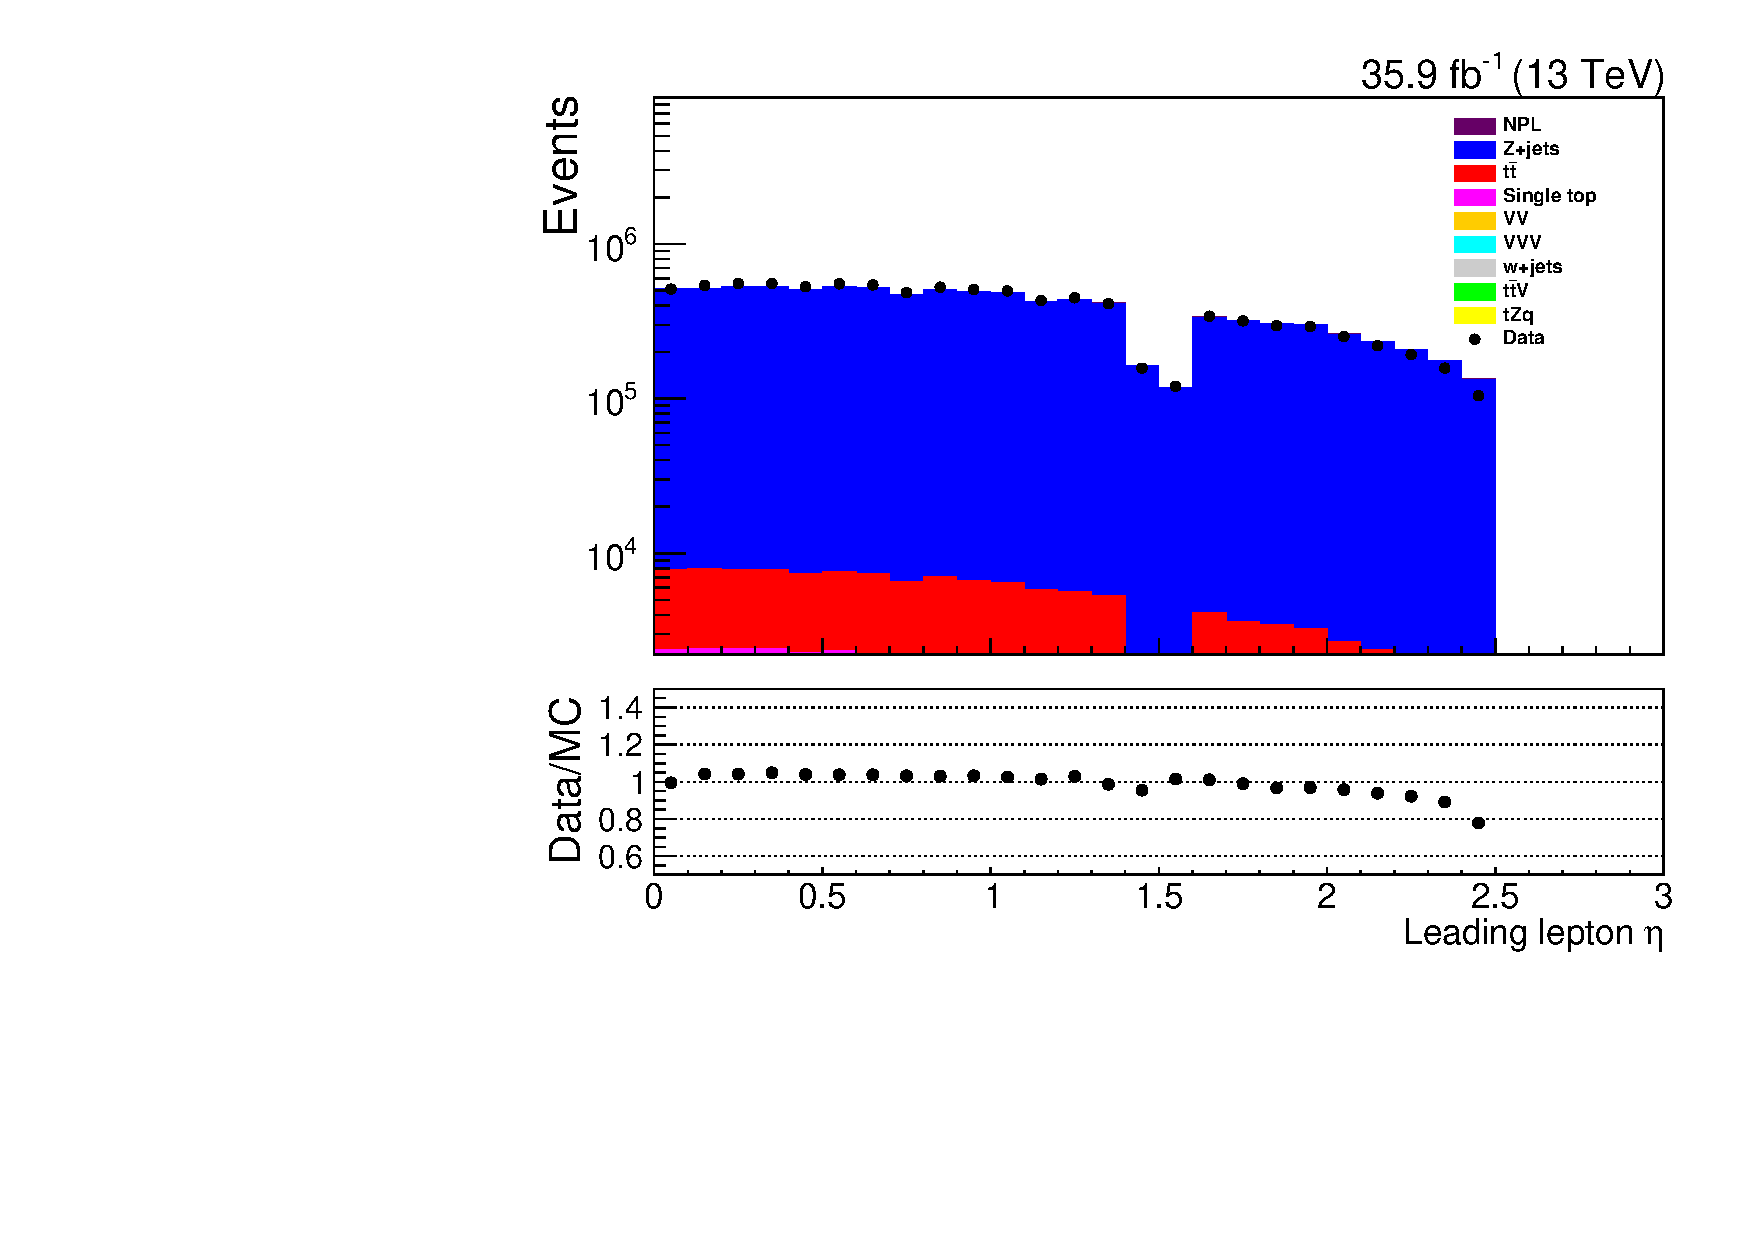
\includegraphics[width=0.47\textwidth]{figs/background-estimation/plots/unblinded/prompt_ee_ttbarInc/lep1Eta_NPL_ee_lepSel_ee_log.pdf}
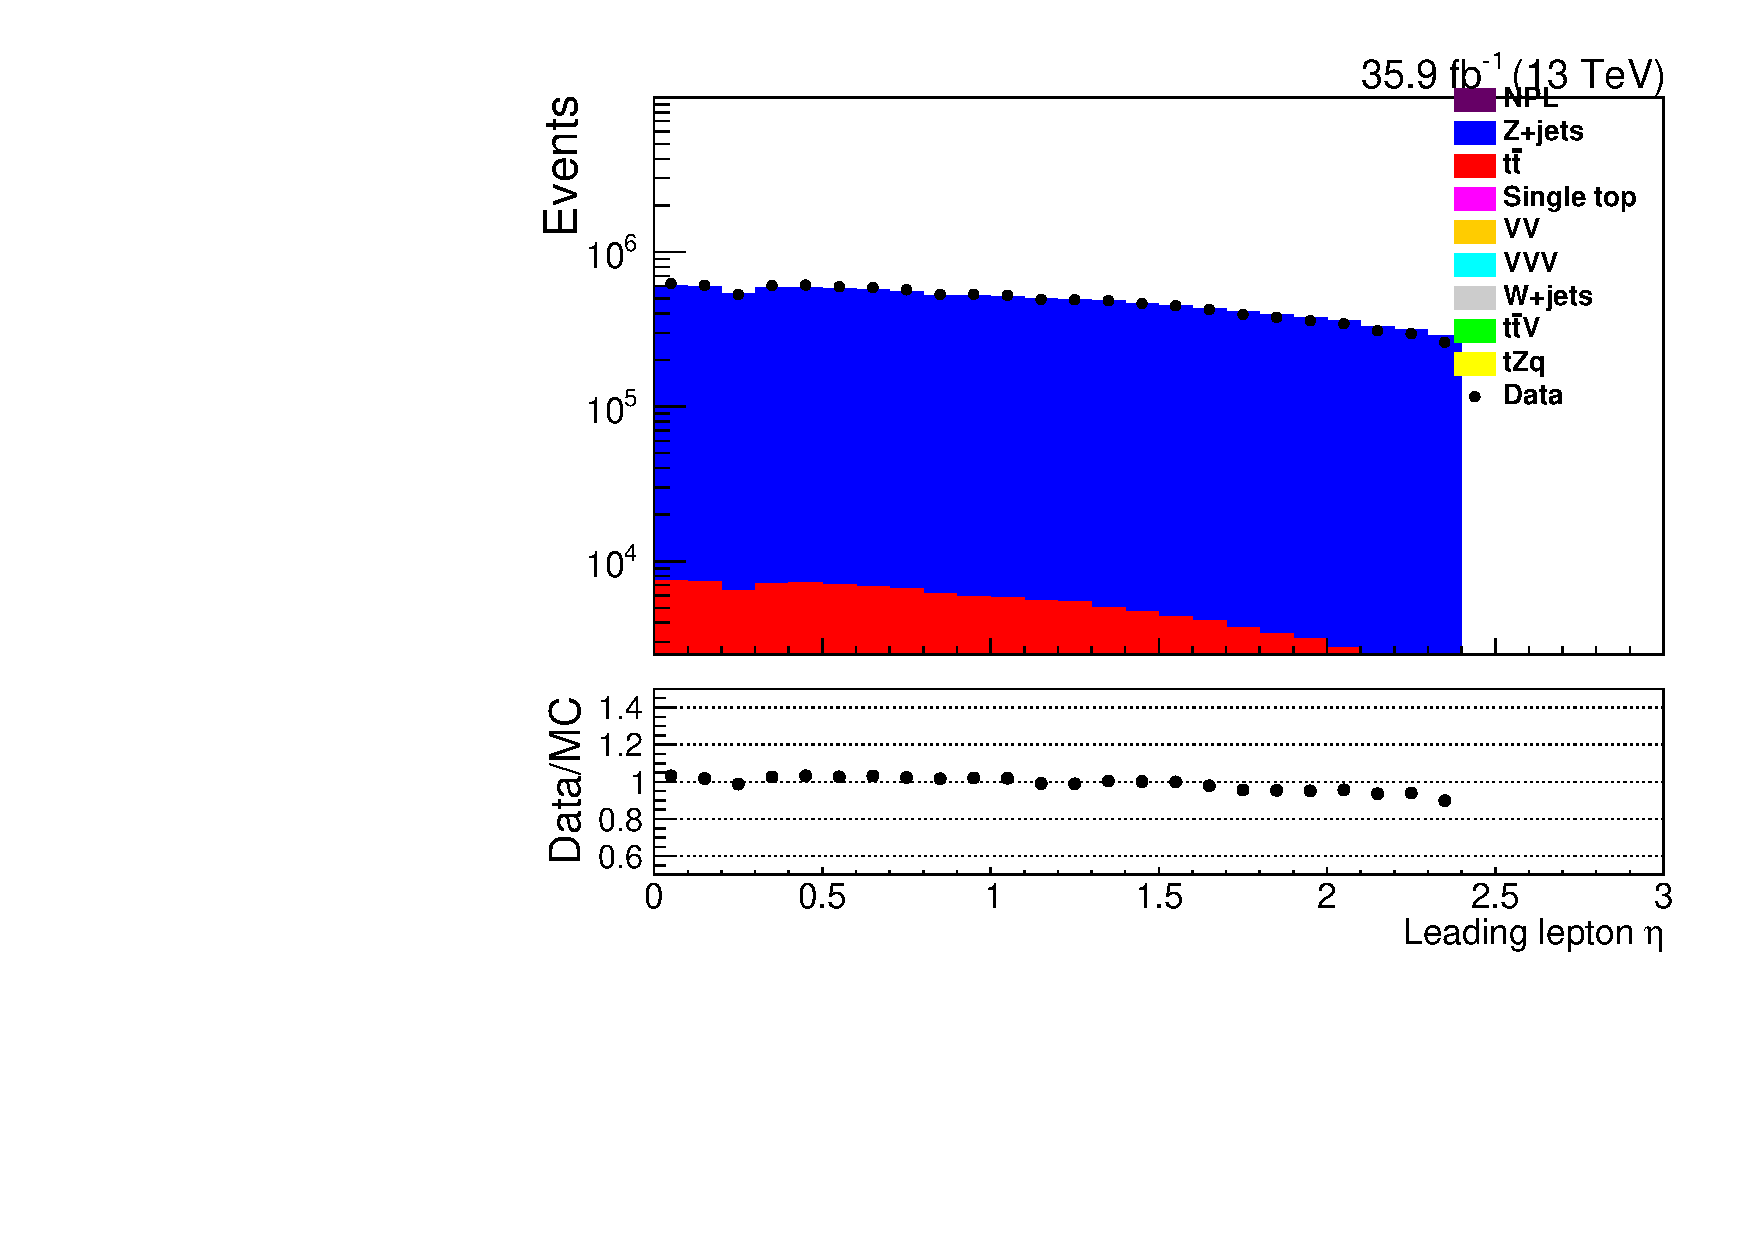
\includegraphics[width=0.47\textwidth]{figs/background-estimation/plots/unblinded/prompt_mumu_ttbarInc/lep1Eta_NPL_mumu_lepSel_mumu_log.pdf}
\\
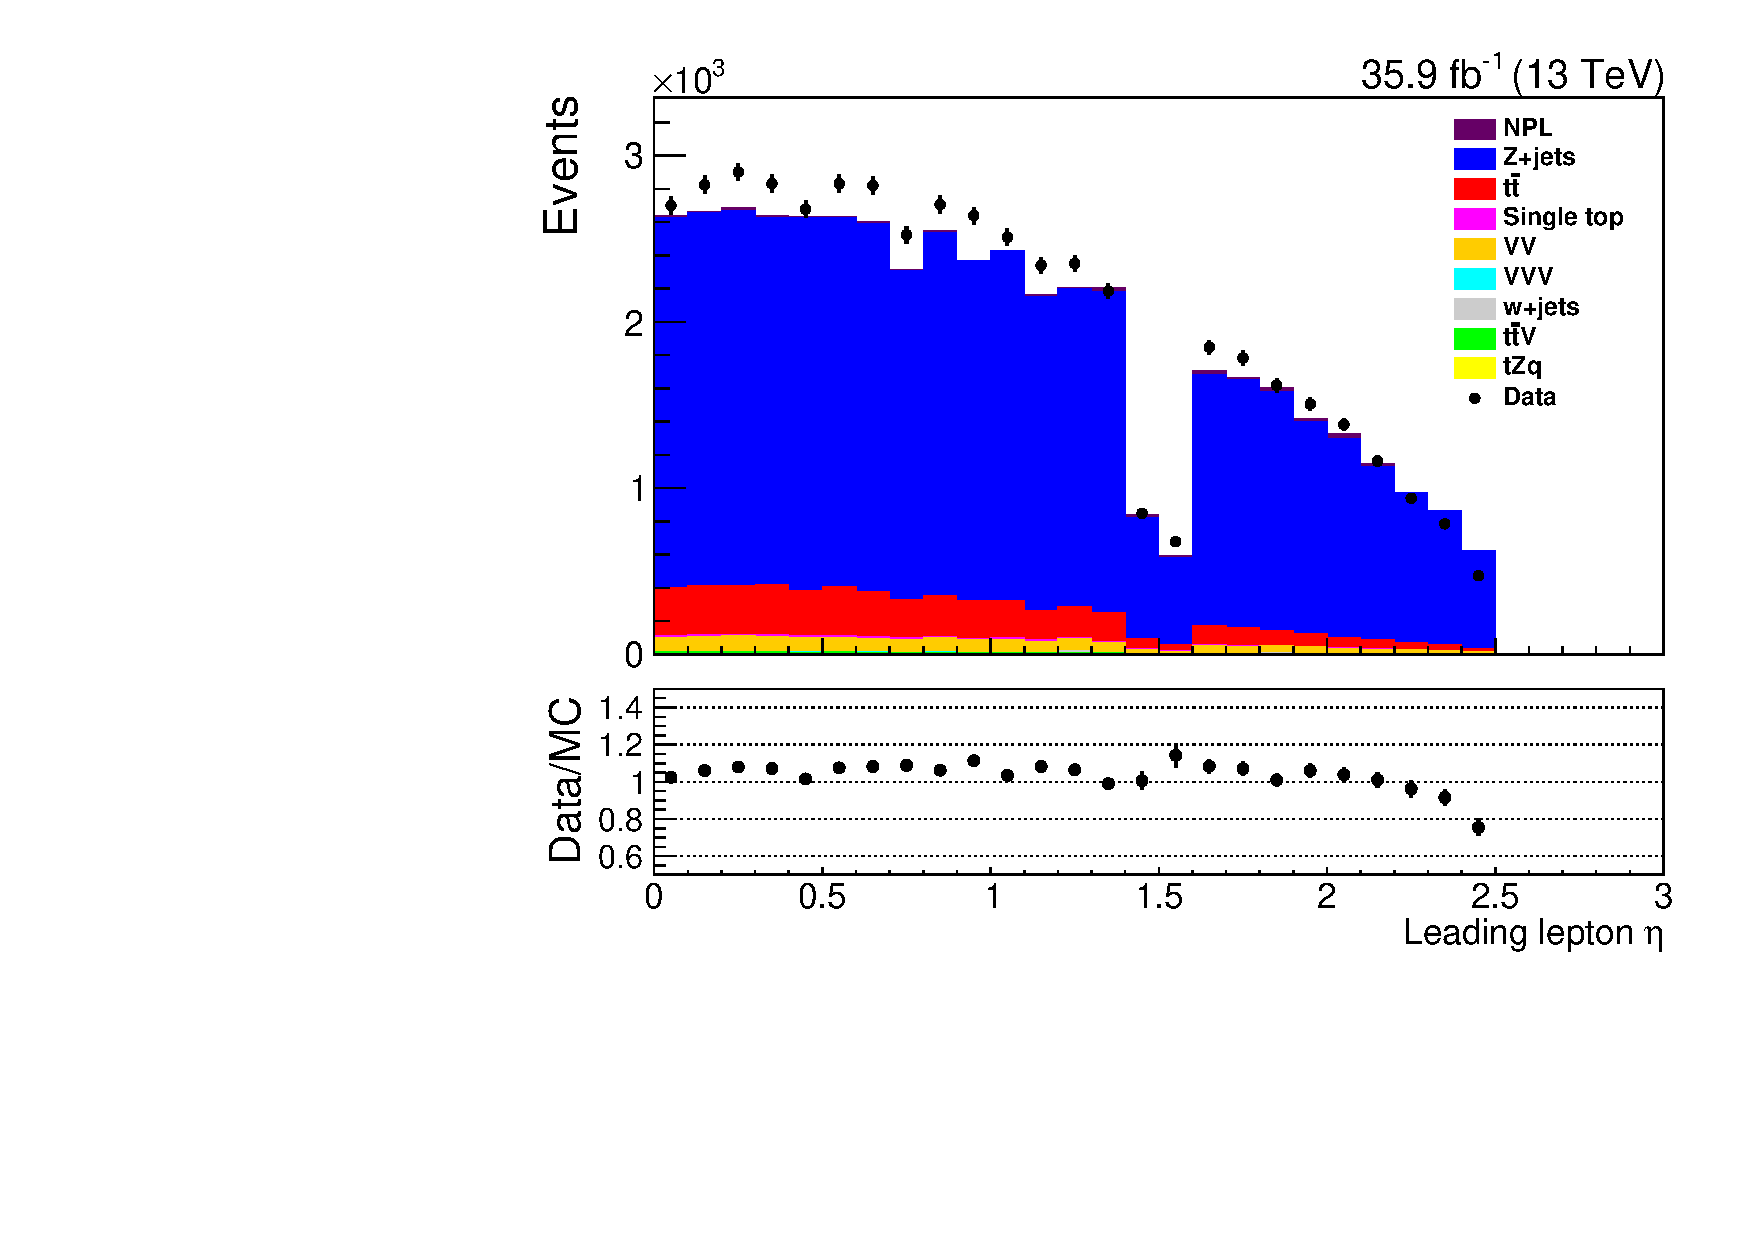
\includegraphics[width=0.47\textwidth]{figs/background-estimation/plots/unblinded/prompt_ee_ttbarInc/lep1Eta_NPL_ee_jetSel_ee.pdf}
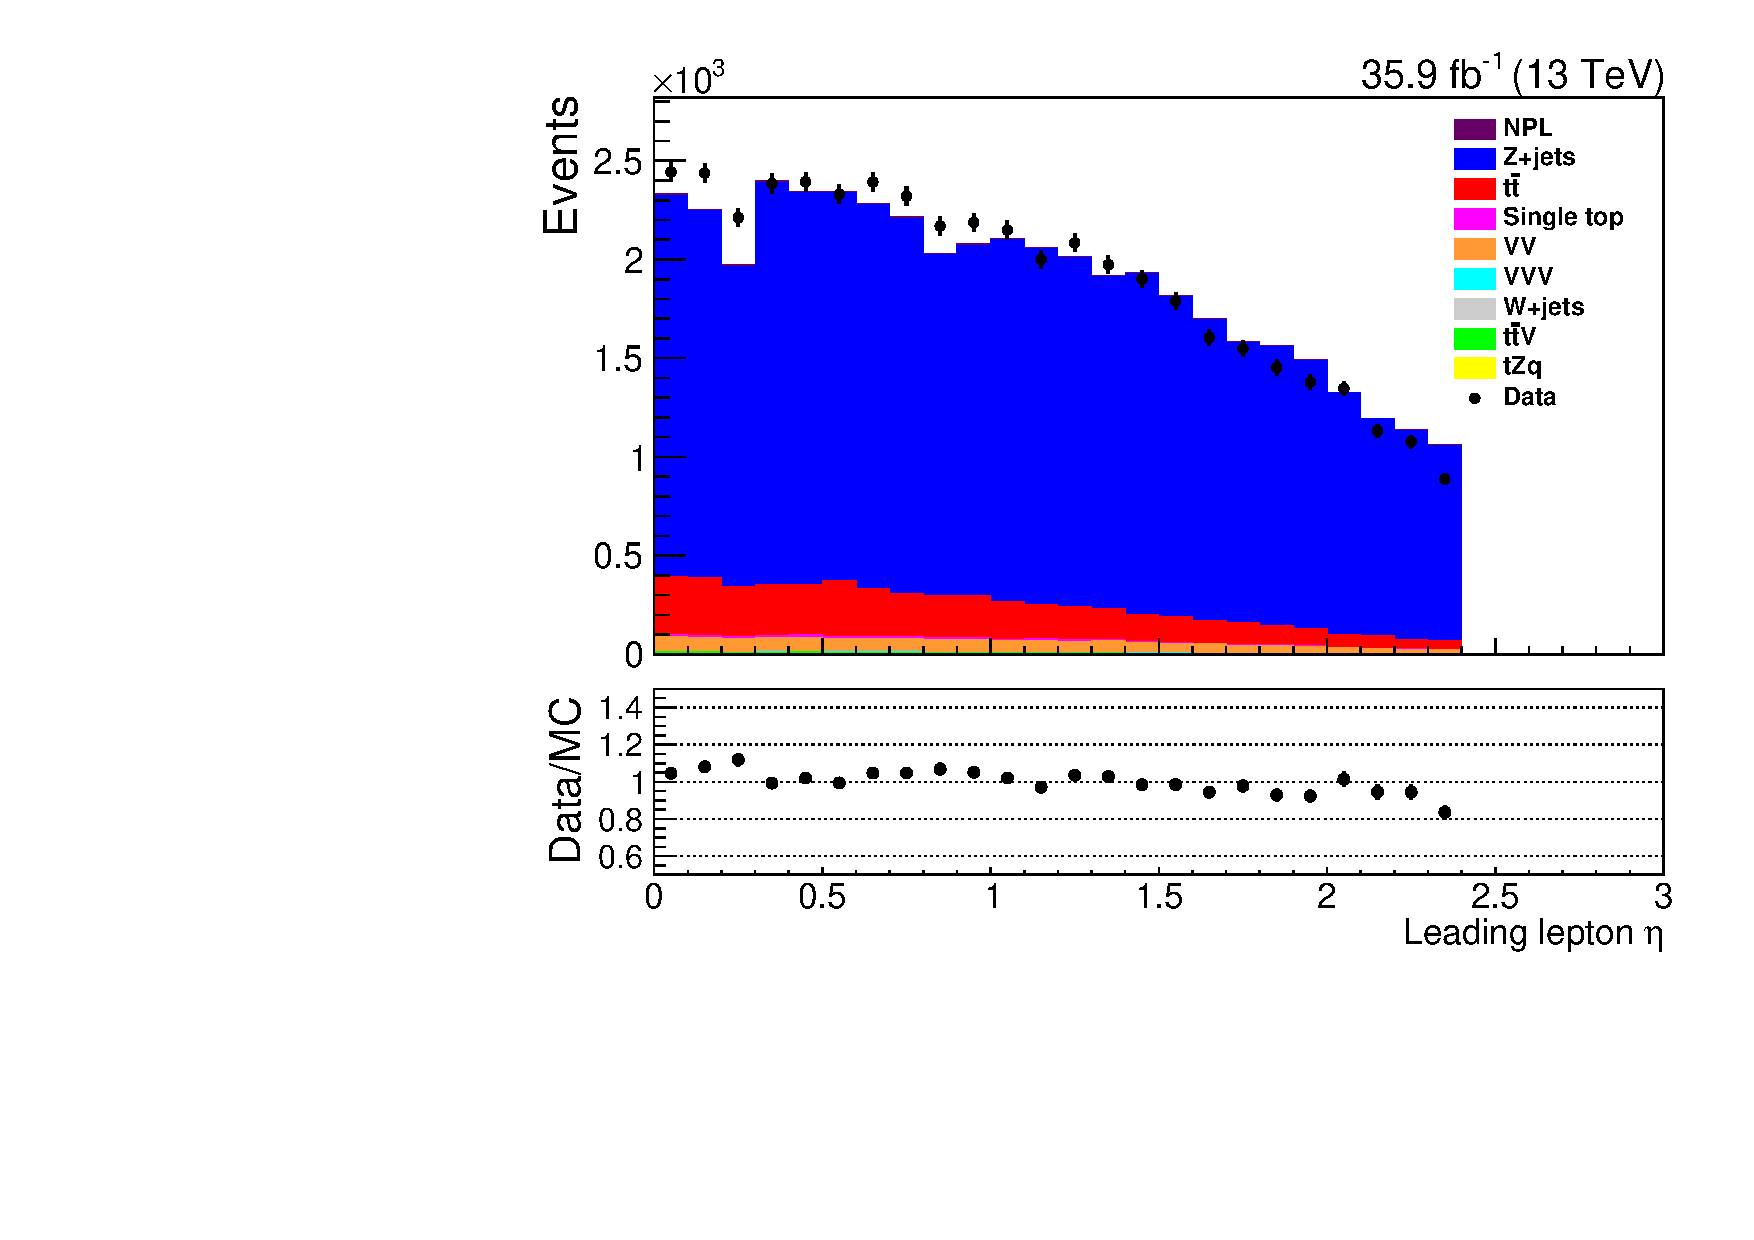
\includegraphics[width=0.47\textwidth]{figs/background-estimation/plots/unblinded/prompt_mumu_ttbarInc/lep1Eta_NPL_mumu_jetSel_mumu.pdf}
\\
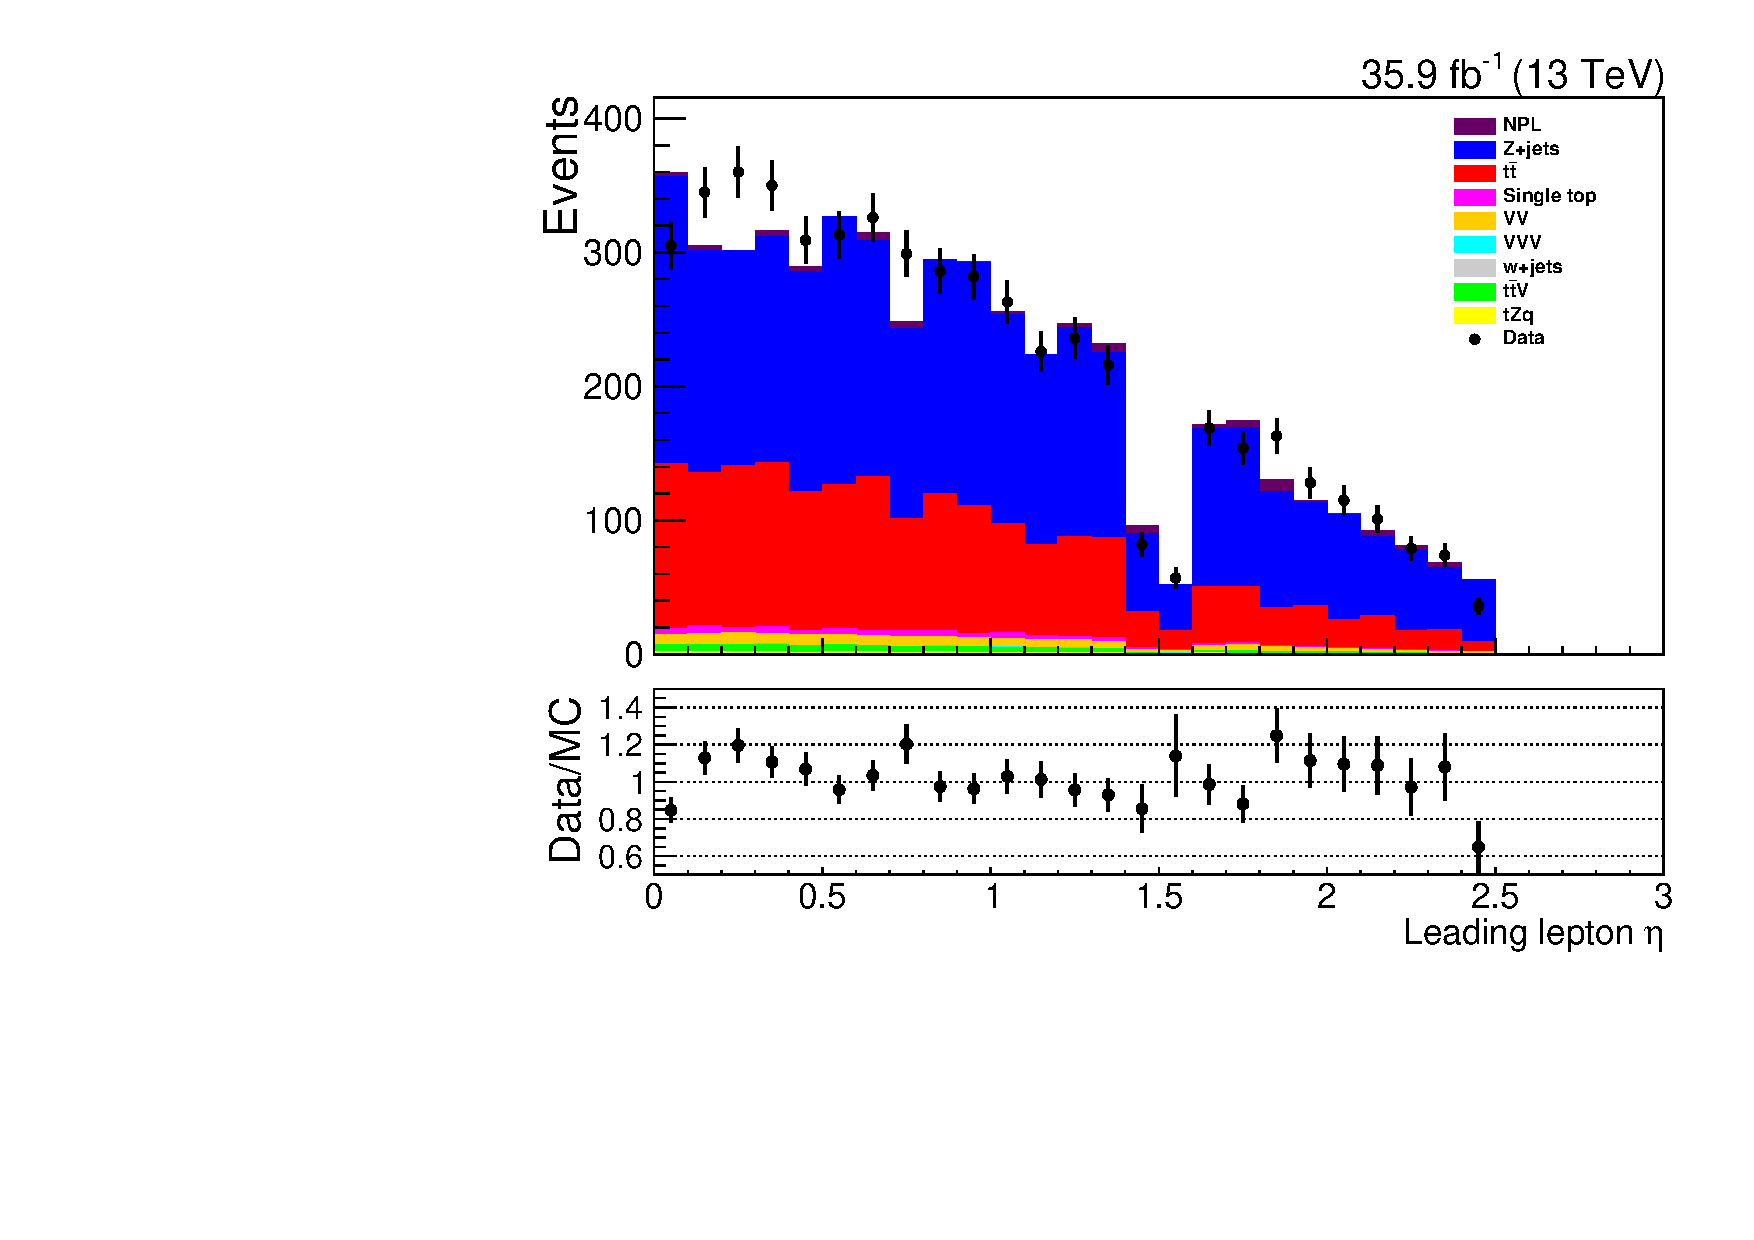
\includegraphics[width=0.47\textwidth]{figs/background-estimation/plots/unblinded/prompt_ee_ttbarInc/lep1Eta_NPL_ee_wMass_ee.pdf}
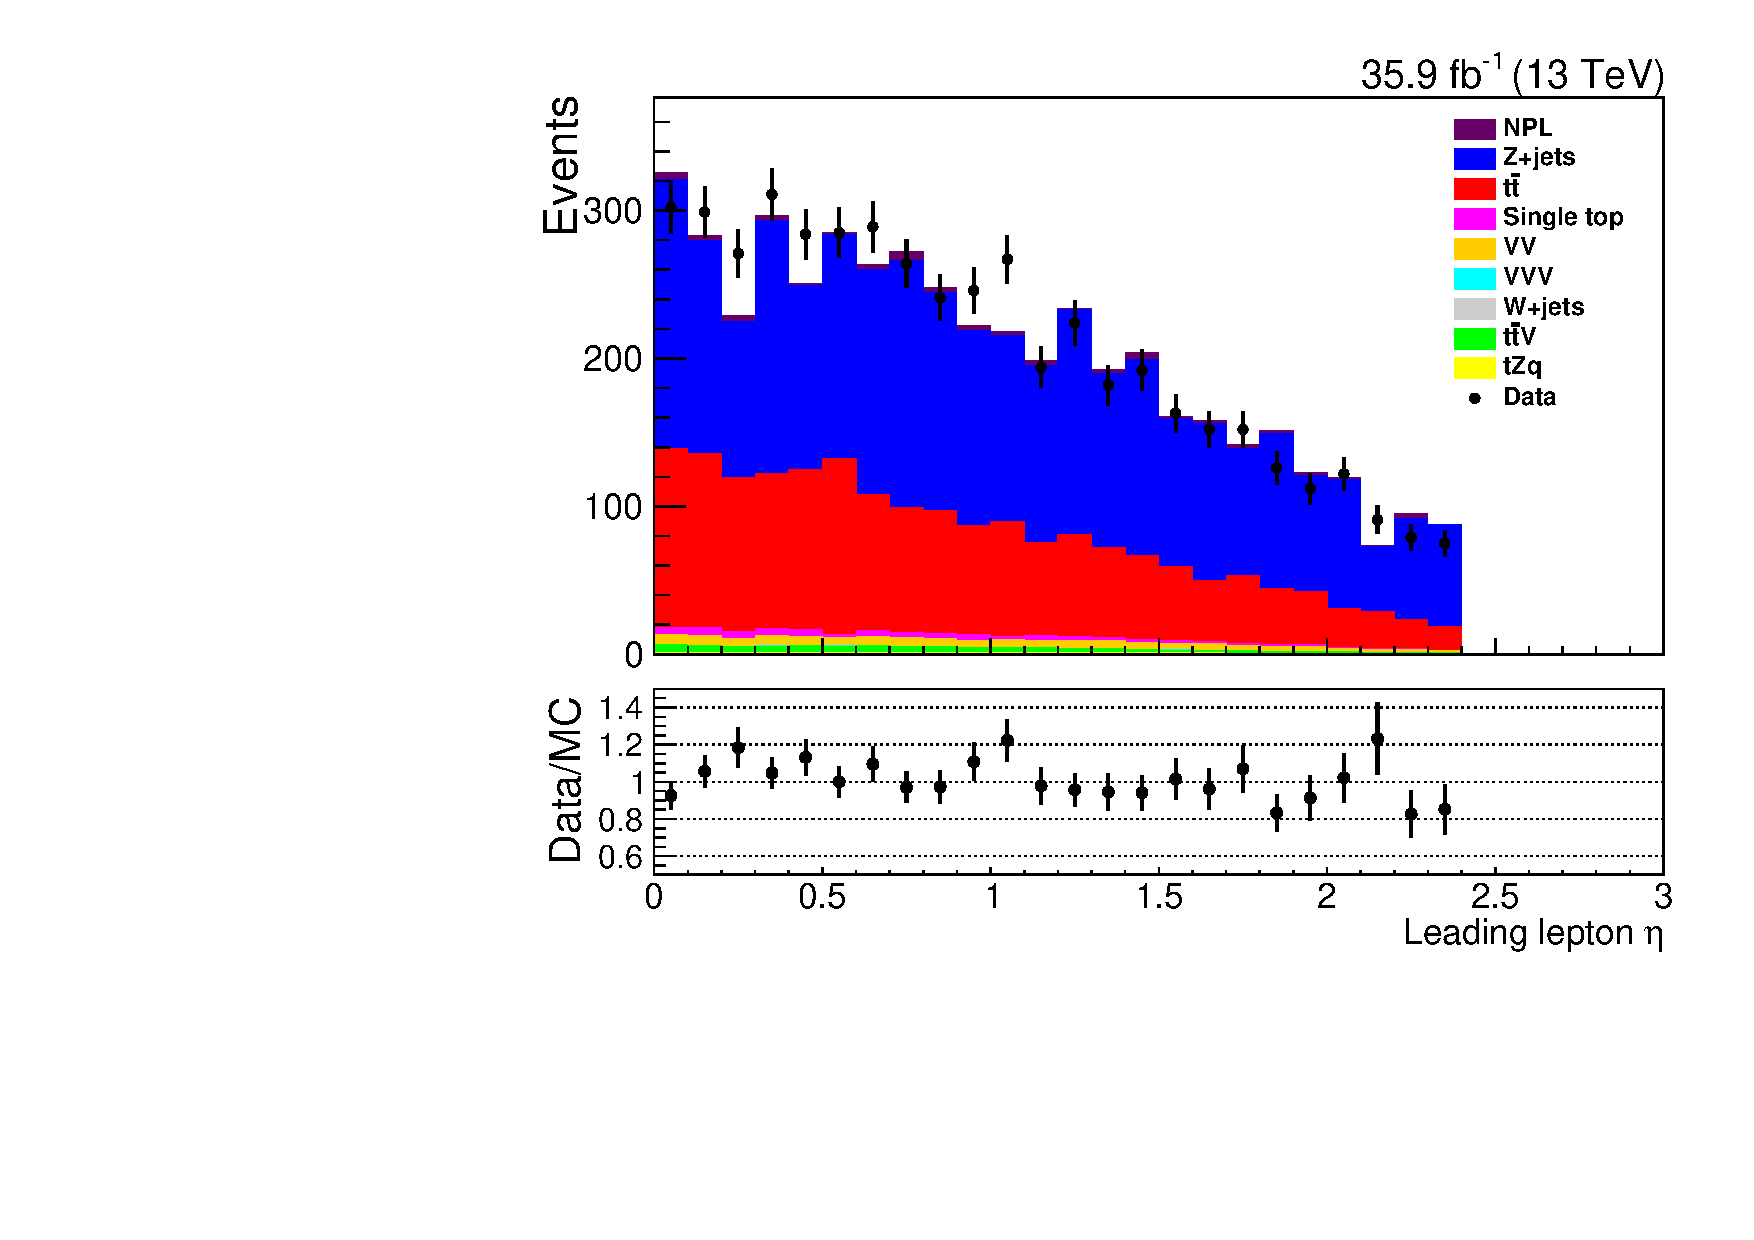
\includegraphics[width=0.47\textwidth]{figs/background-estimation/plots/unblinded/prompt_mumu_ttbarInc/lep1Eta_NPL_mumu_wMass_mumu.pdf}
\caption{
The leading lepton $\eta$ following only the lepton selection criteria and simulation corrections (top), the jet selection criteria (middle) and all of the signal region selection criteria (bottom).
}
\label{fig:SR_lep1Eta}
\end{figure}

\begin{figure}[h]
\centering
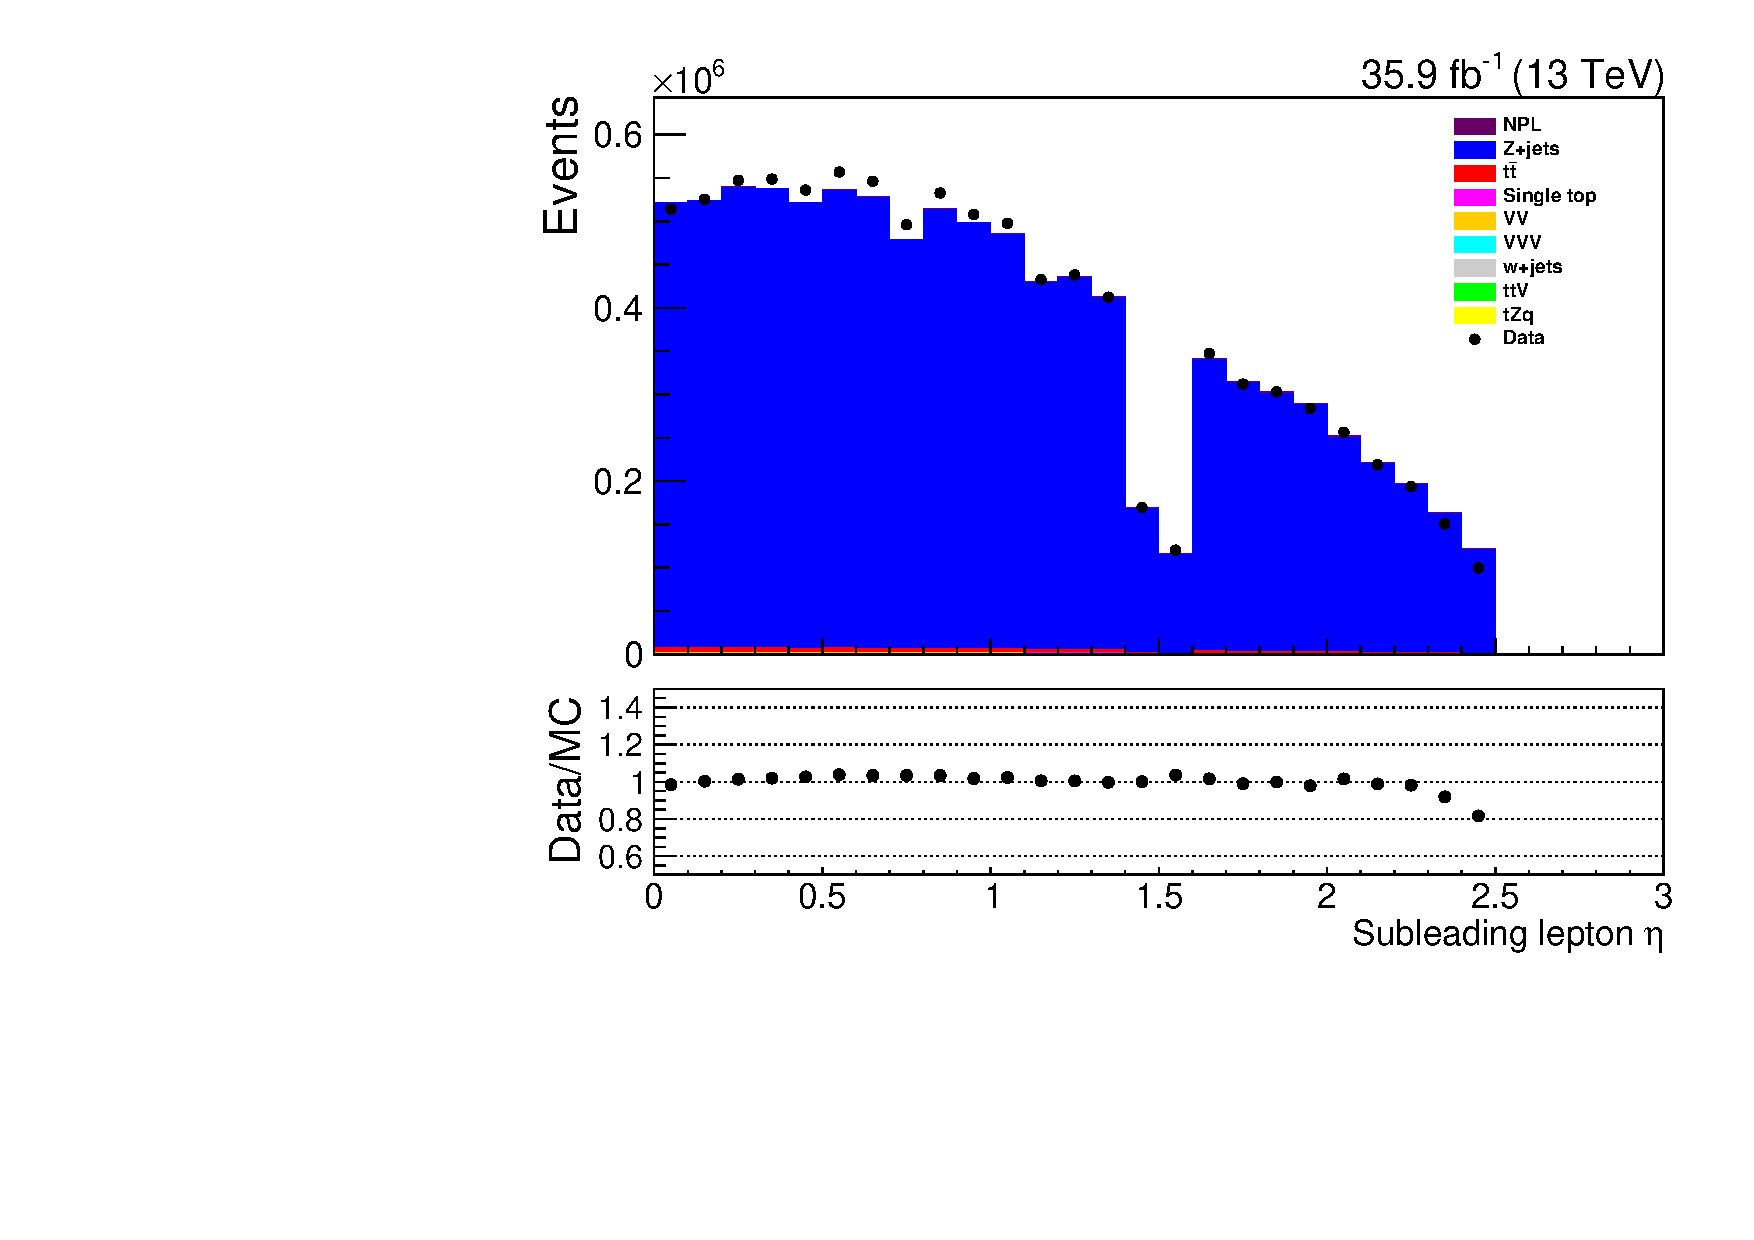
\includegraphics[width=0.47\textwidth]{figs/background-estimation/plots/unblinded/prompt_ee_ttbarInc/lep2Eta_NPL_ee_lepSel_ee_log.pdf}
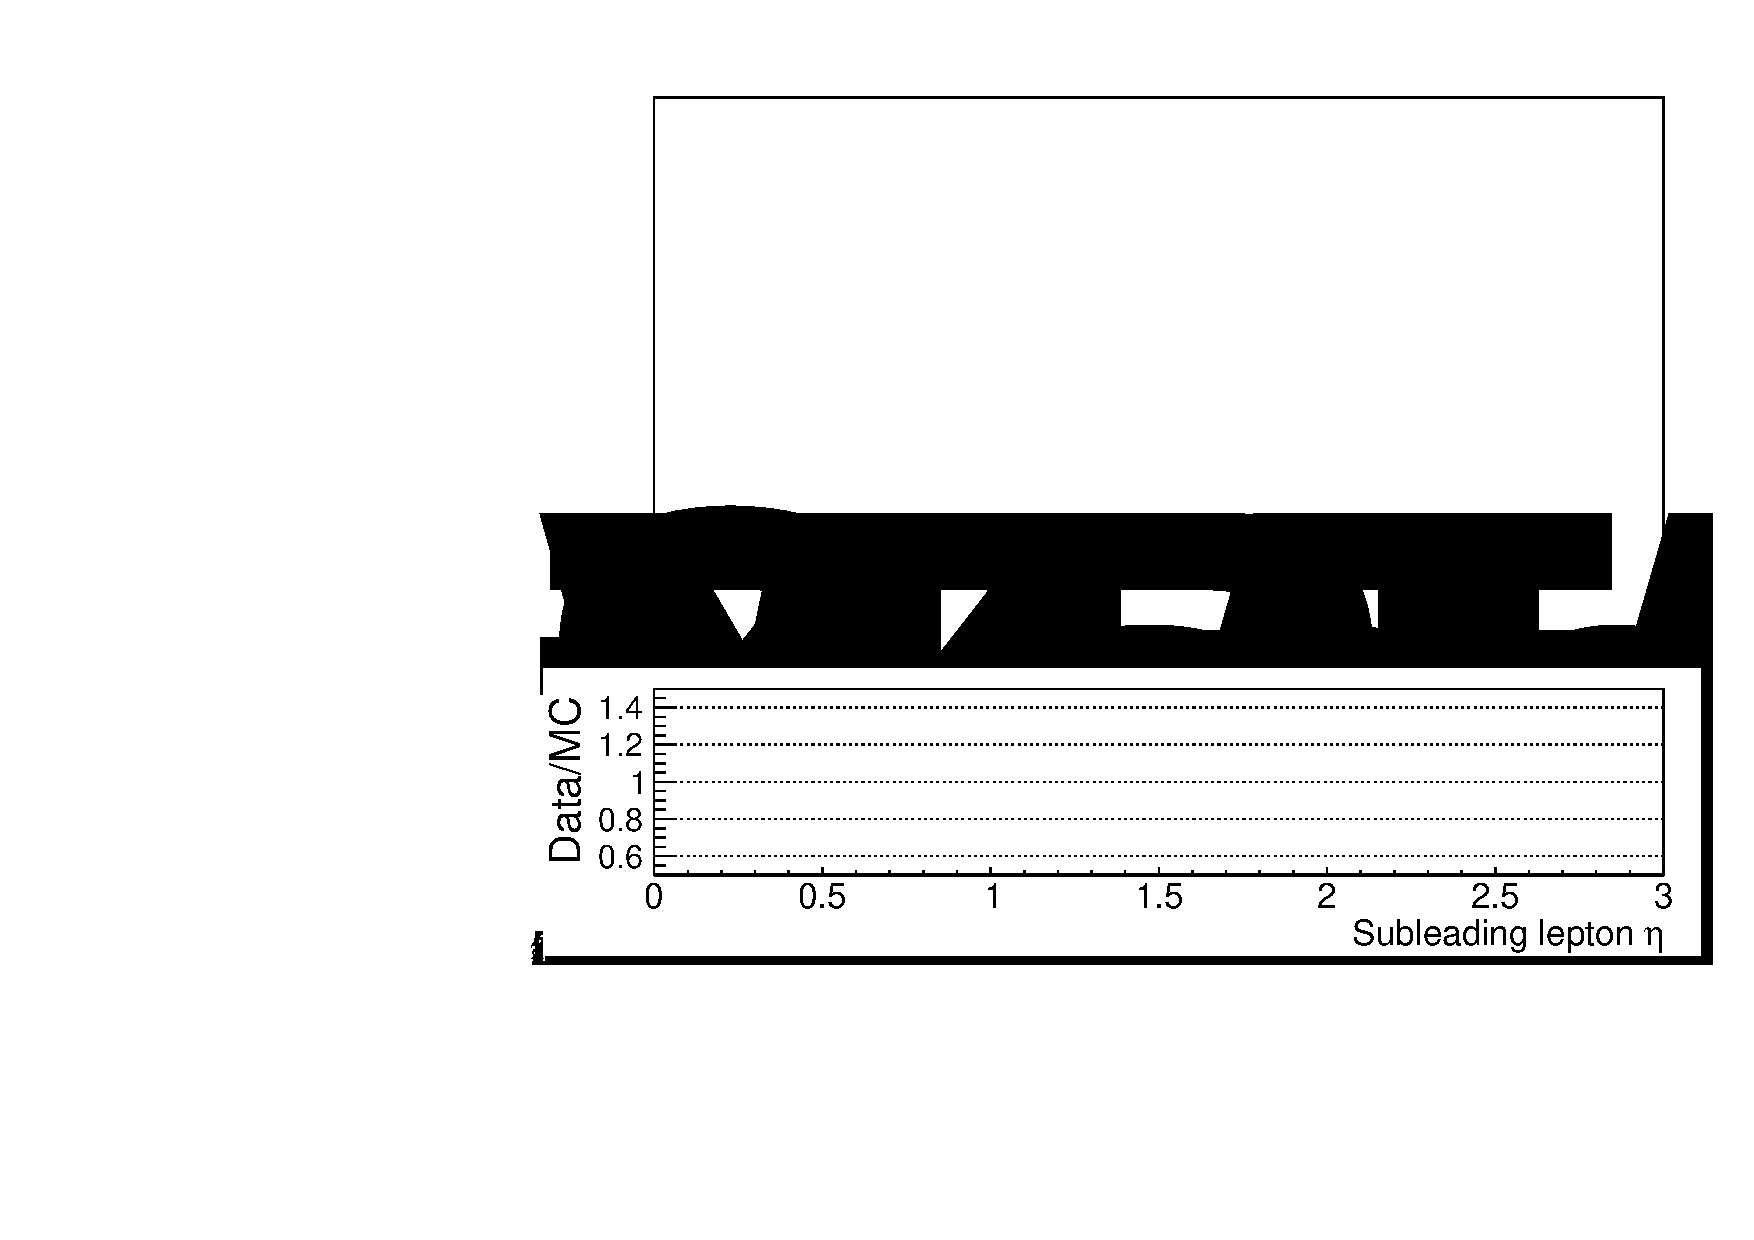
\includegraphics[width=0.47\textwidth]{figs/background-estimation/plots/unblinded/prompt_mumu_ttbarInc/lep2Eta_NPL_mumu_lepSel_mumu_log.pdf}
\\
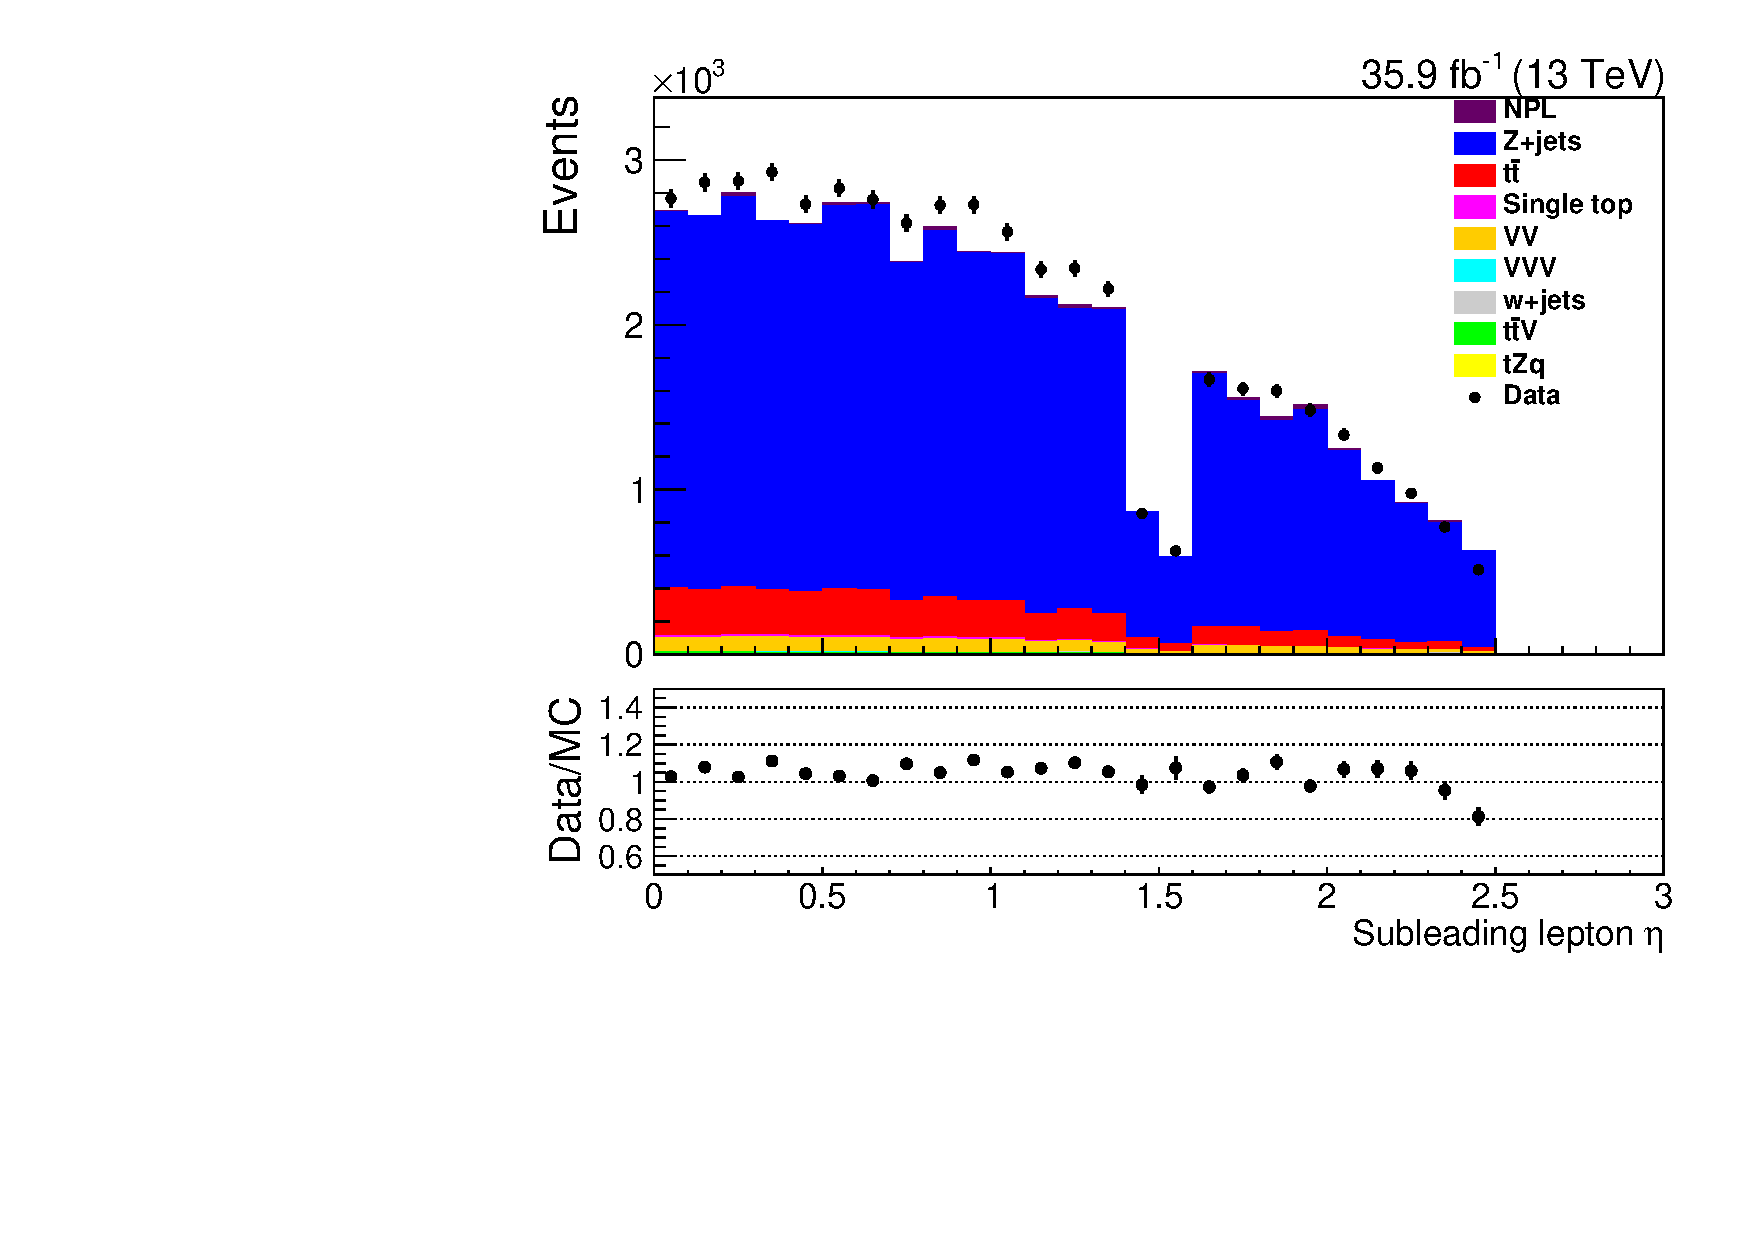
\includegraphics[width=0.47\textwidth]{figs/background-estimation/plots/unblinded/prompt_ee_ttbarInc/lep2Eta_NPL_ee_jetSel_ee.pdf}
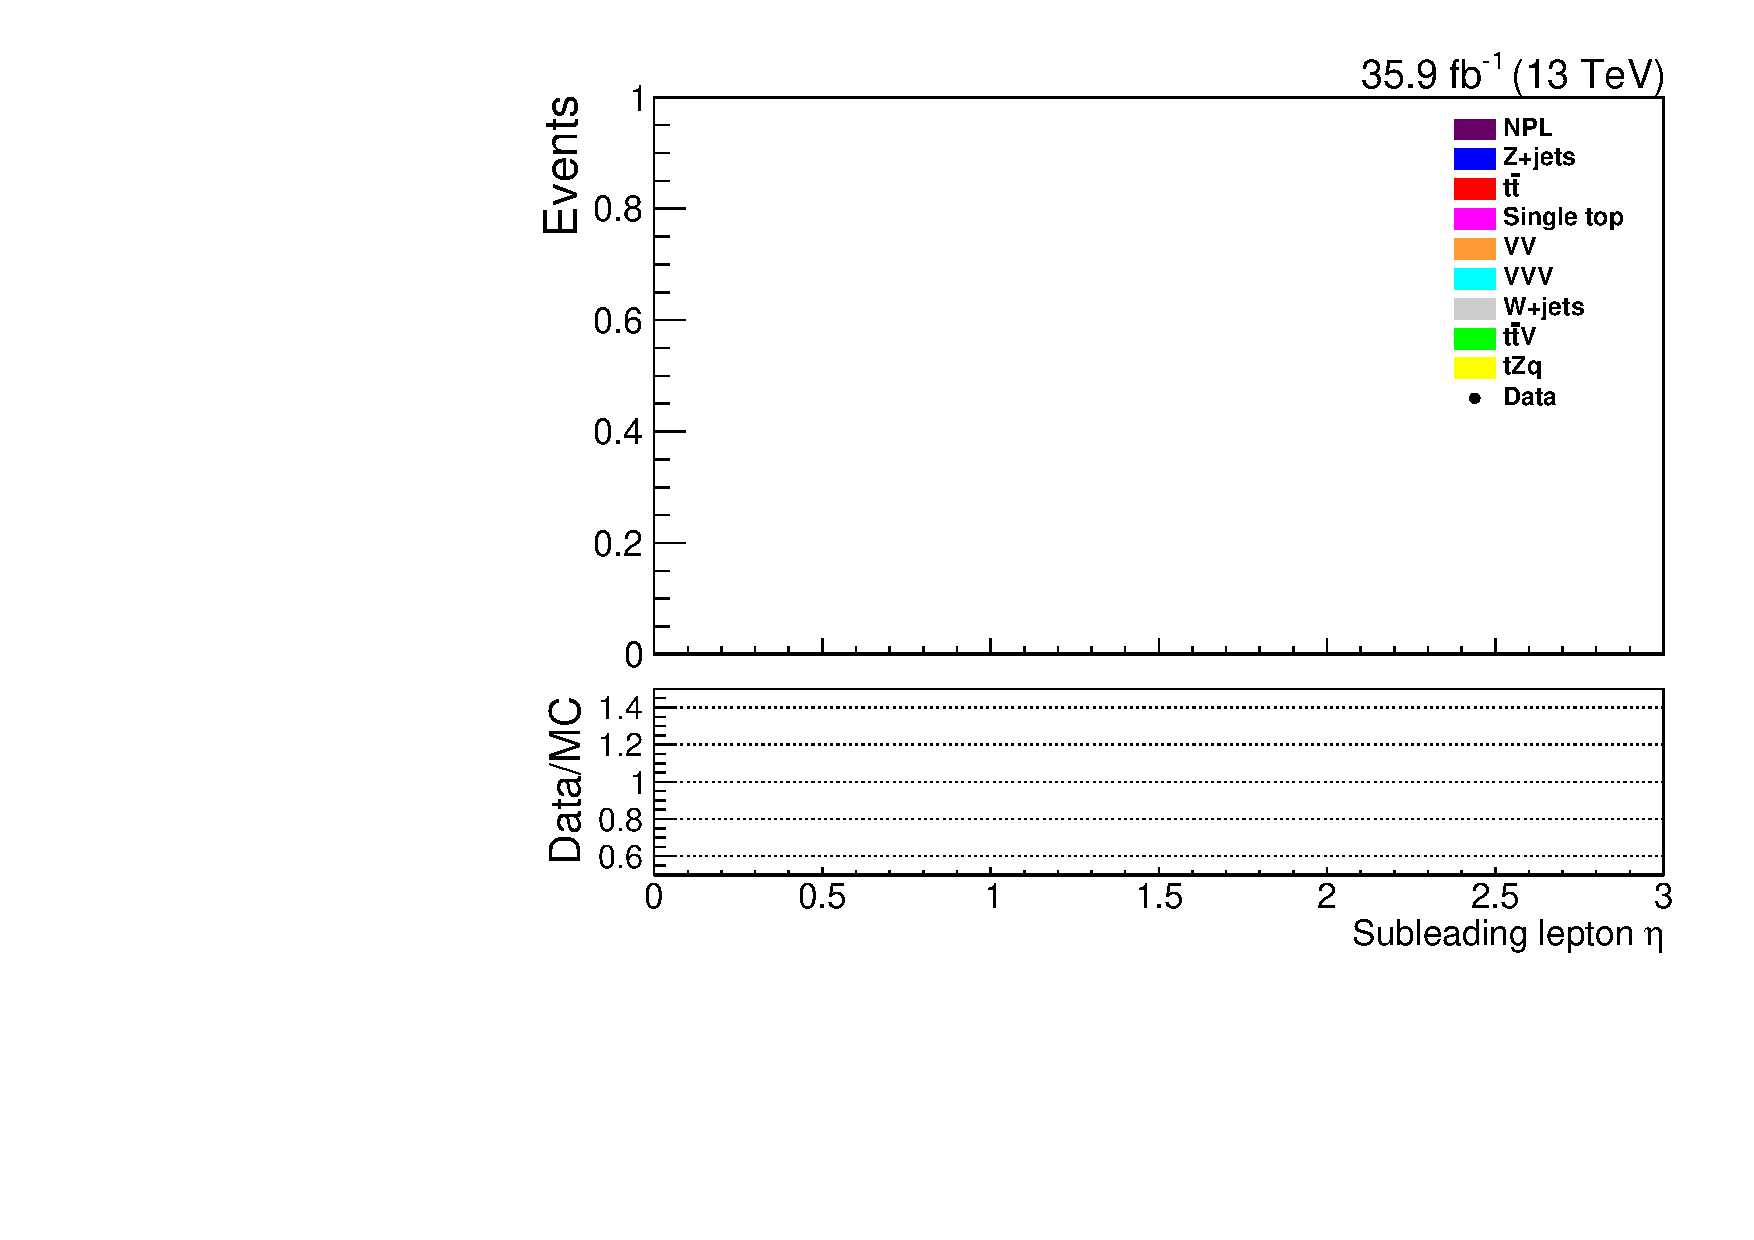
\includegraphics[width=0.47\textwidth]{figs/background-estimation/plots/unblinded/prompt_mumu_ttbarInc/lep2Eta_NPL_mumu_jetSel_mumu.pdf}
\\
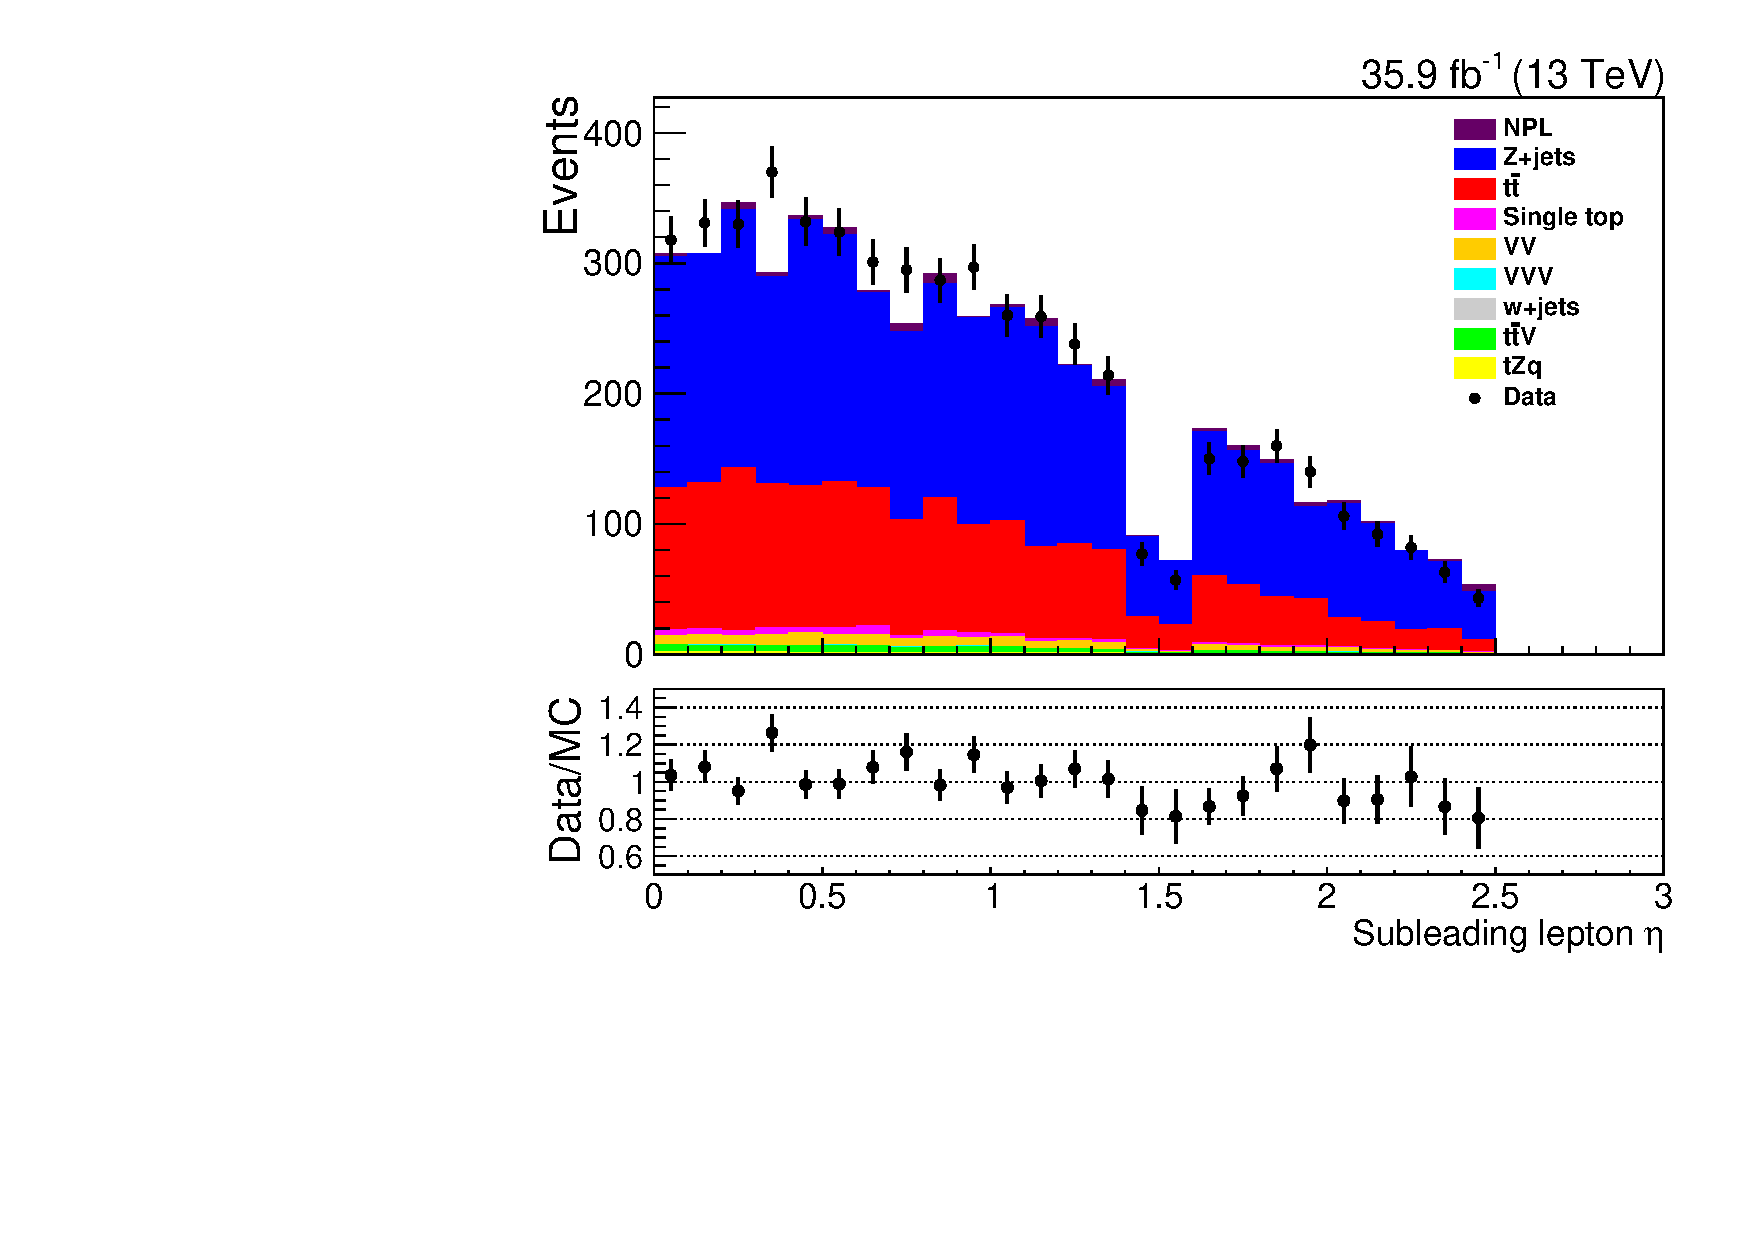
\includegraphics[width=0.47\textwidth]{figs/background-estimation/plots/unblinded/prompt_ee_ttbarInc/lep2Eta_NPL_ee_wMass_ee.pdf}
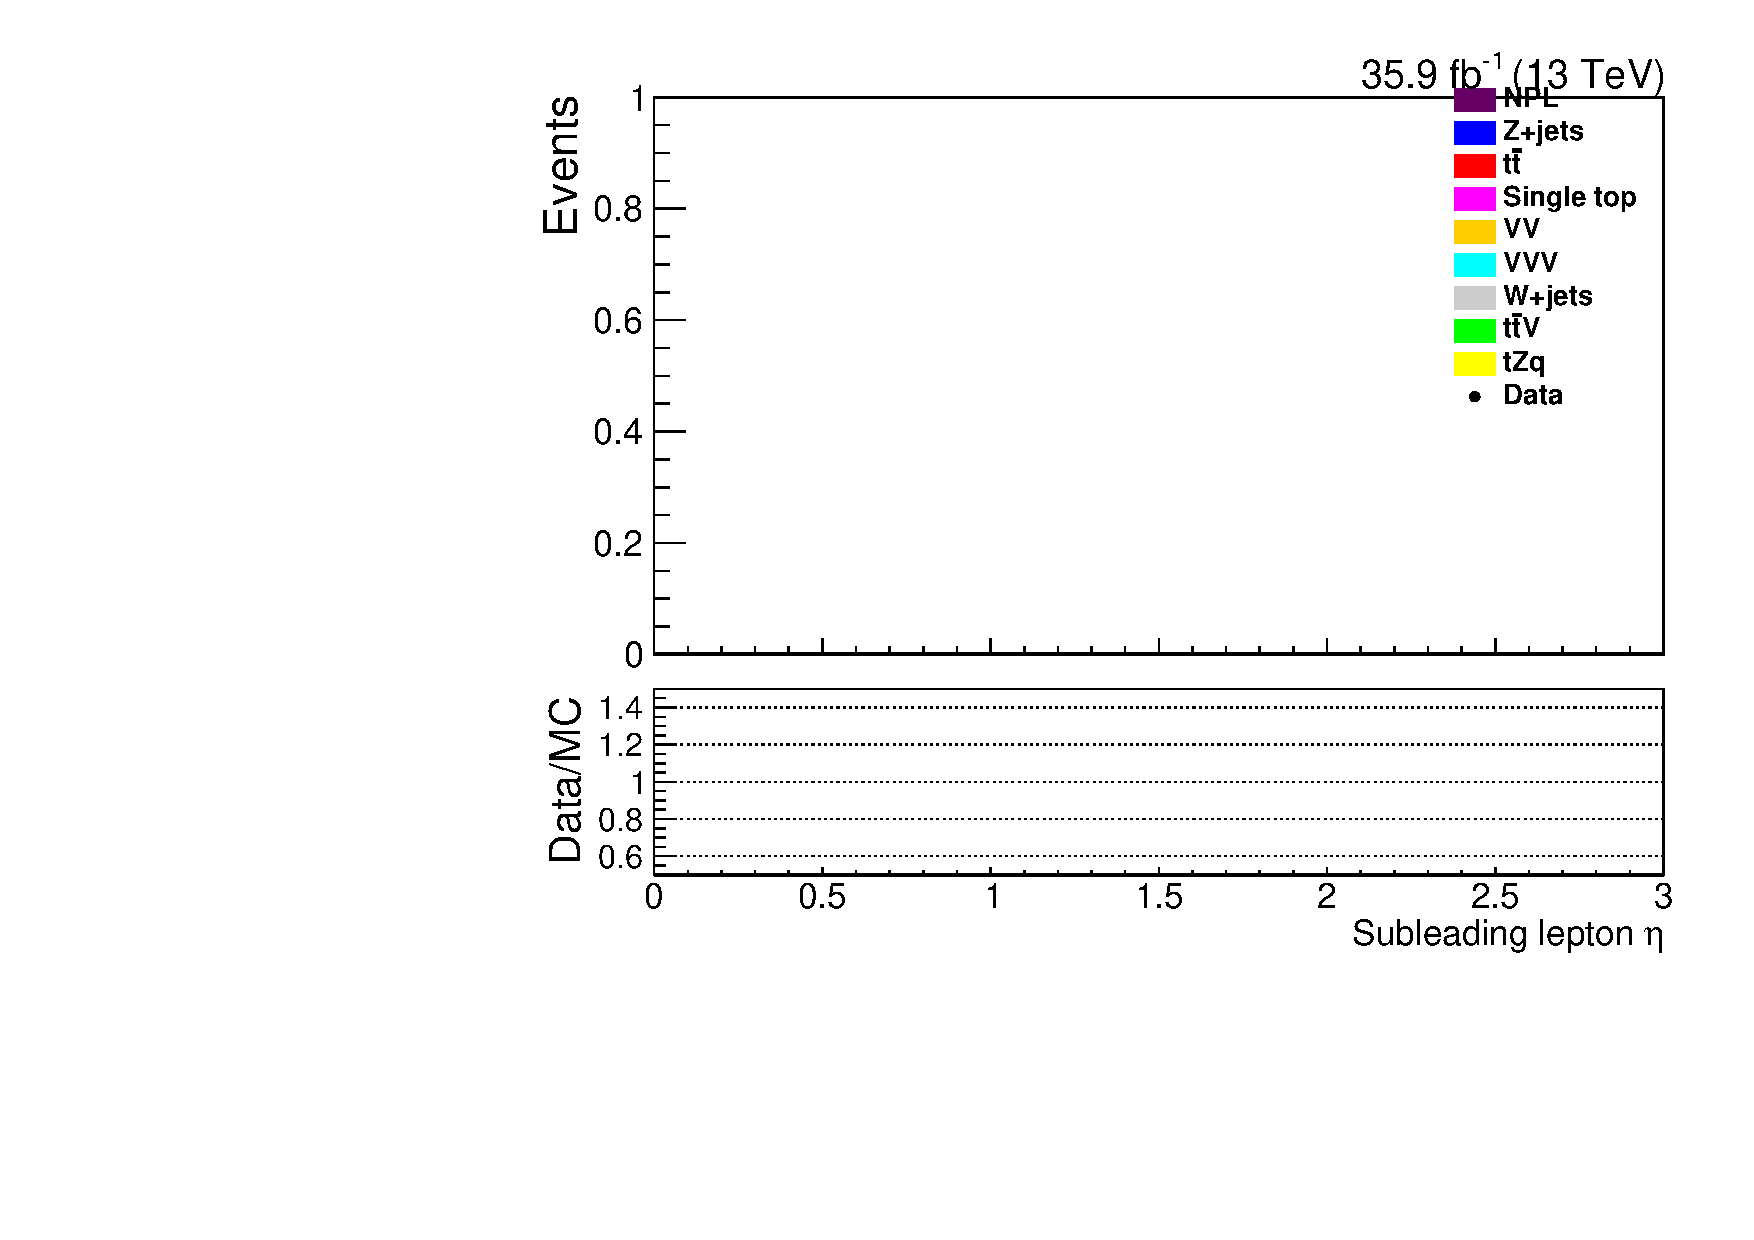
\includegraphics[width=0.47\textwidth]{figs/background-estimation/plots/unblinded/prompt_mumu_ttbarInc/lep2Eta_NPL_mumu_wMass_mumu.pdf}
\caption{
The subleading lepton $\eta$ following only the lepton selection criteria and simulation corrections (top), the jet selection criteria (middle) and all of the signal region selection criteria (bottom).
}
\label{fig:SR_lep2Eta}
\end{figure}

\begin{figure}[h]
\centering
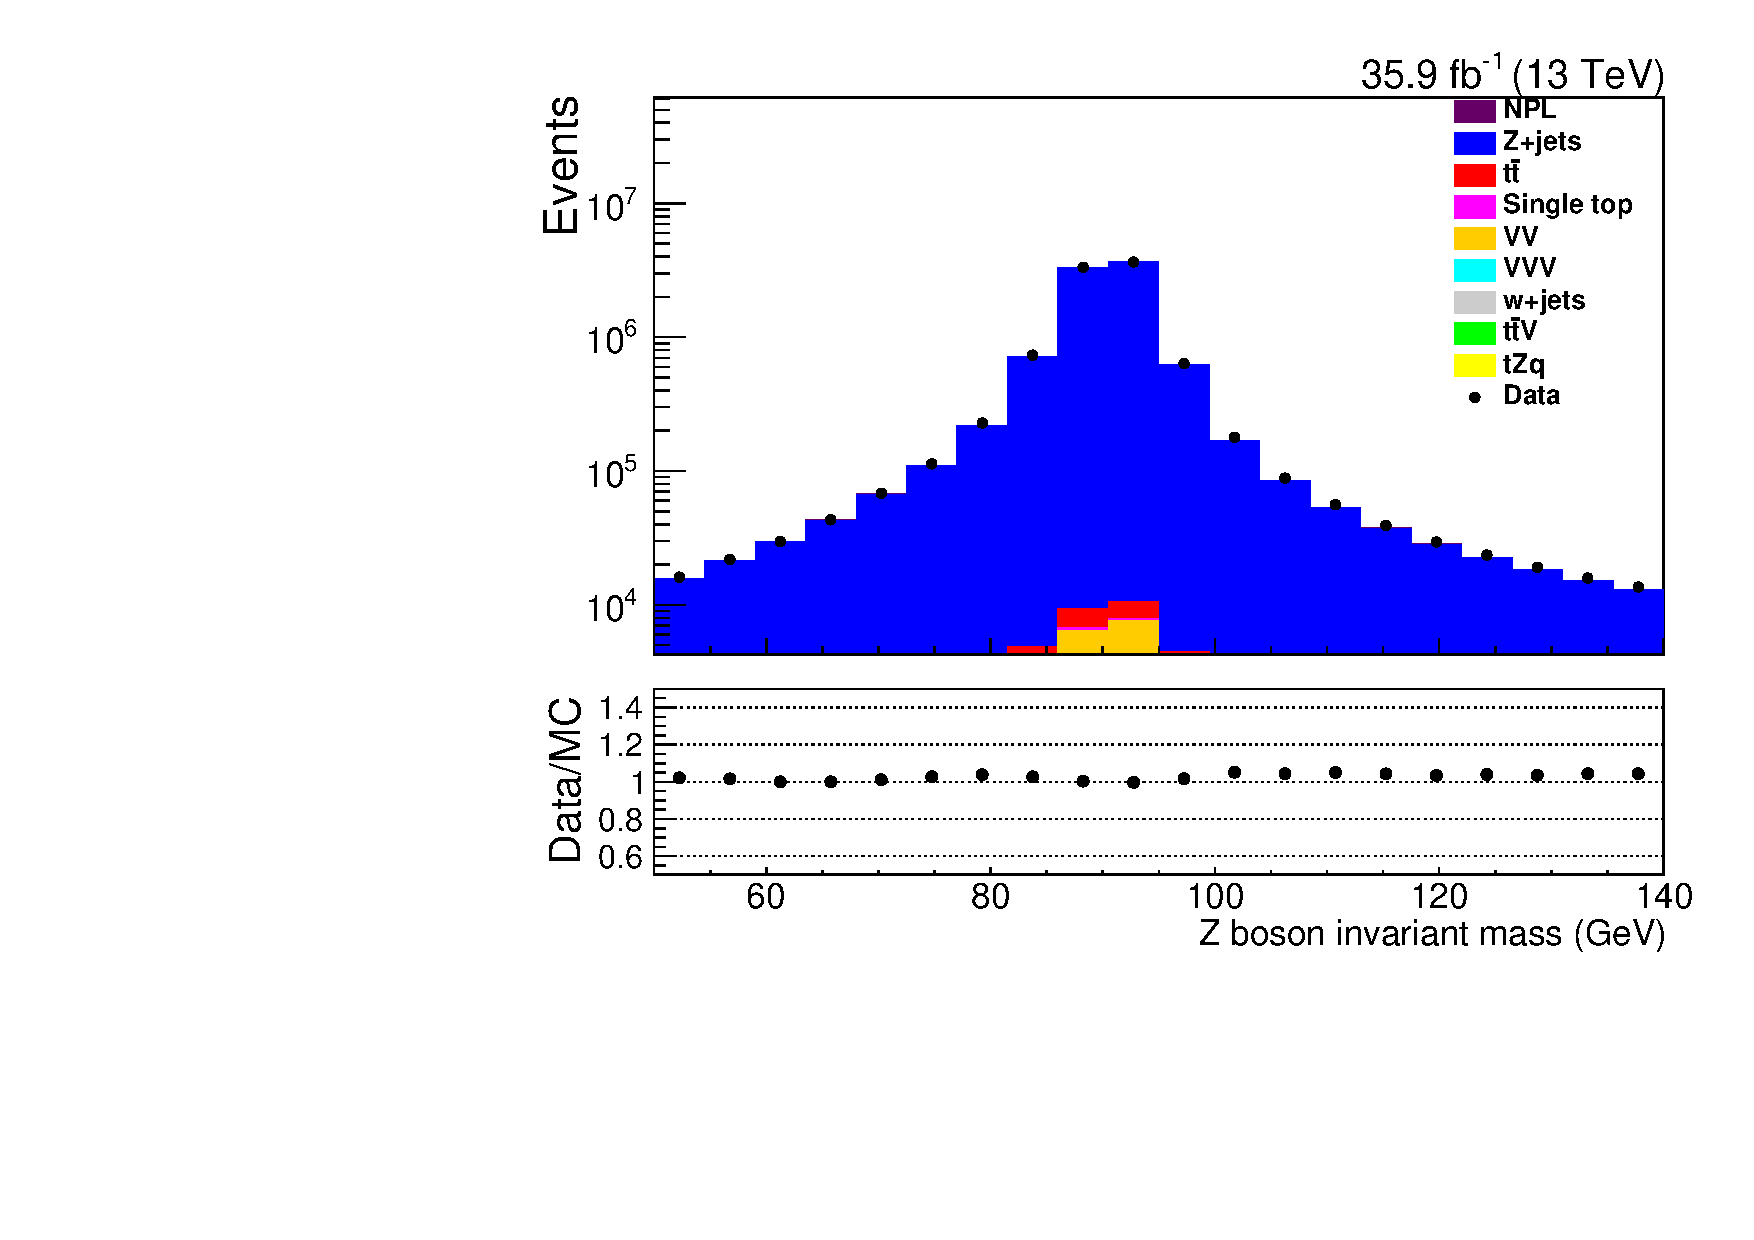
\includegraphics[width=0.47\textwidth]{figs/background-estimation/plots/unblinded/prompt_ee_ttbarInc/zPairMass_NPL_ee_lepSel_ee_log.pdf}
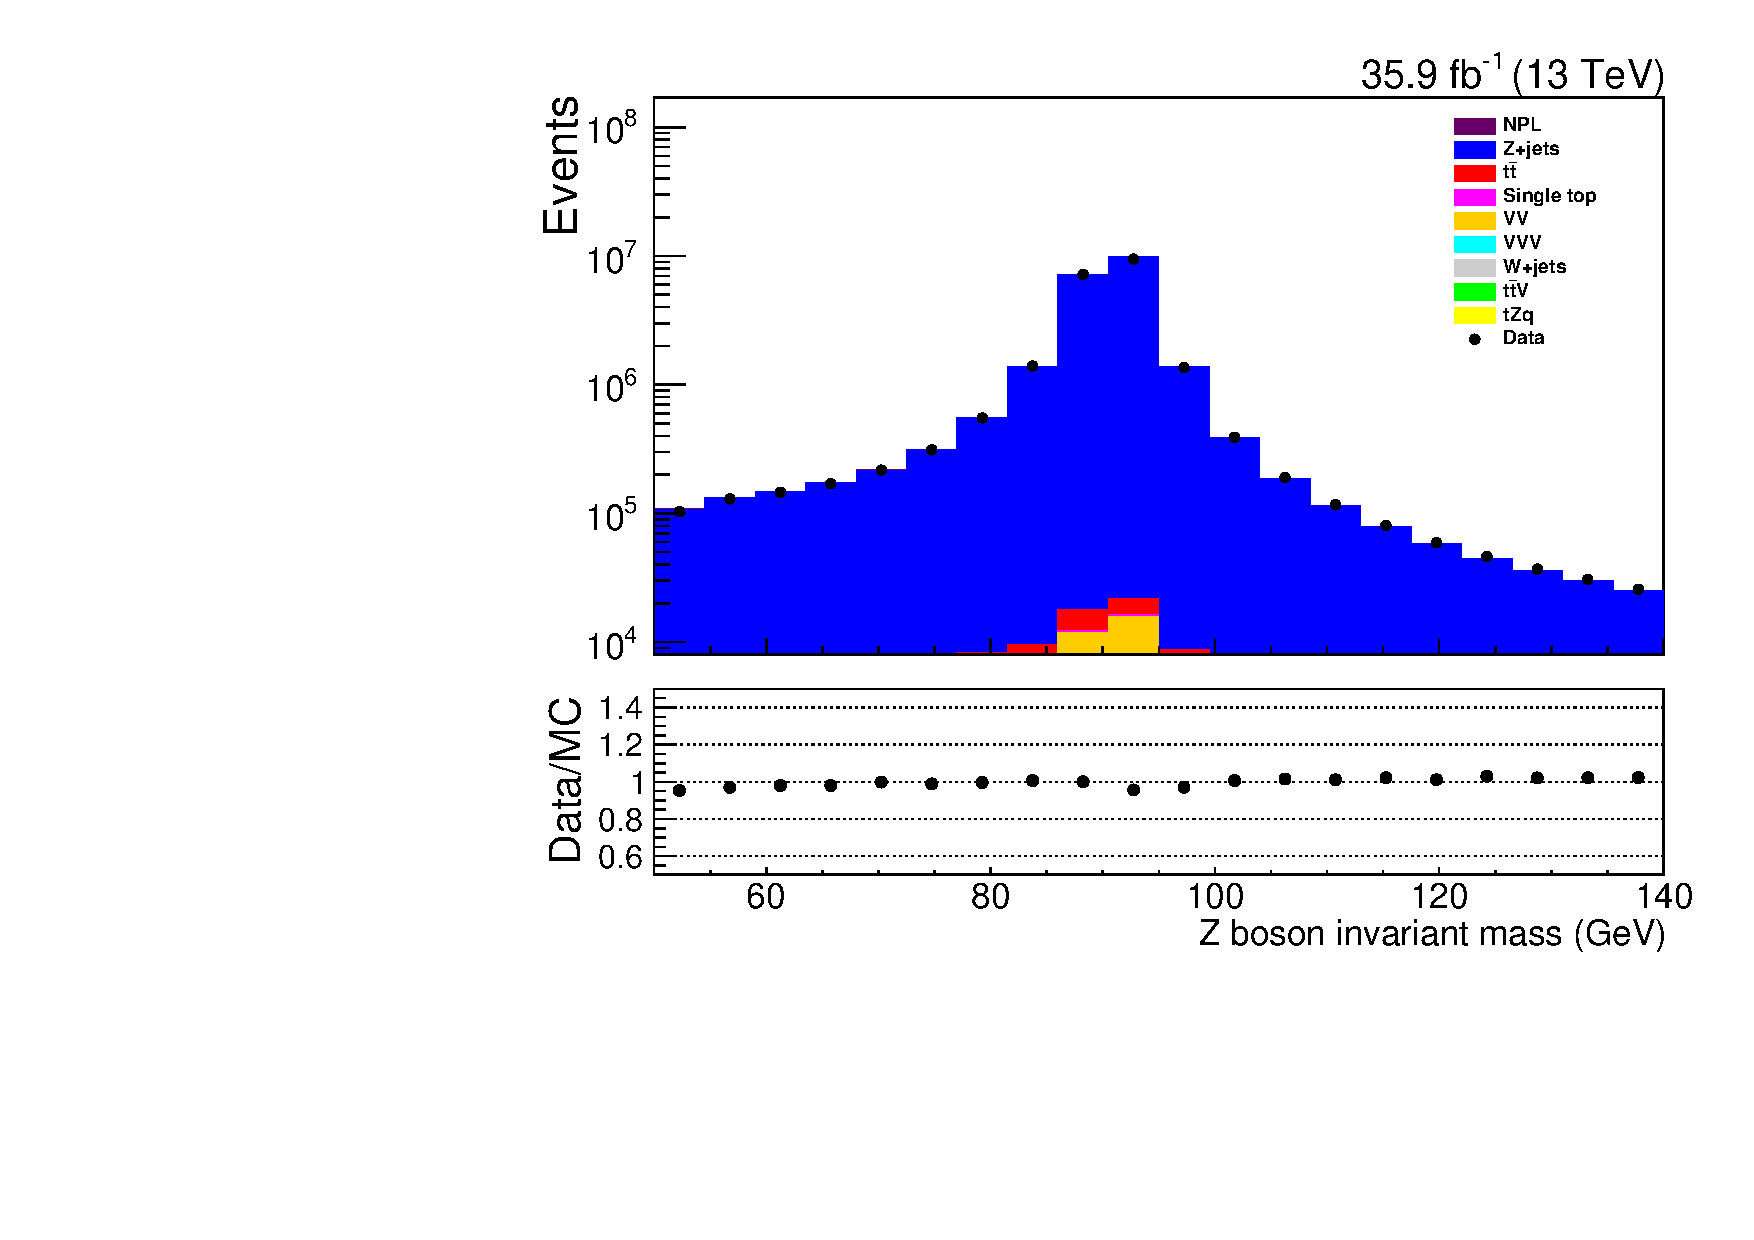
\includegraphics[width=0.47\textwidth]{figs/background-estimation/plots/unblinded/prompt_mumu_ttbarInc/zPairMass_NPL_mumu_lepSel_mumu_log.pdf}
\\
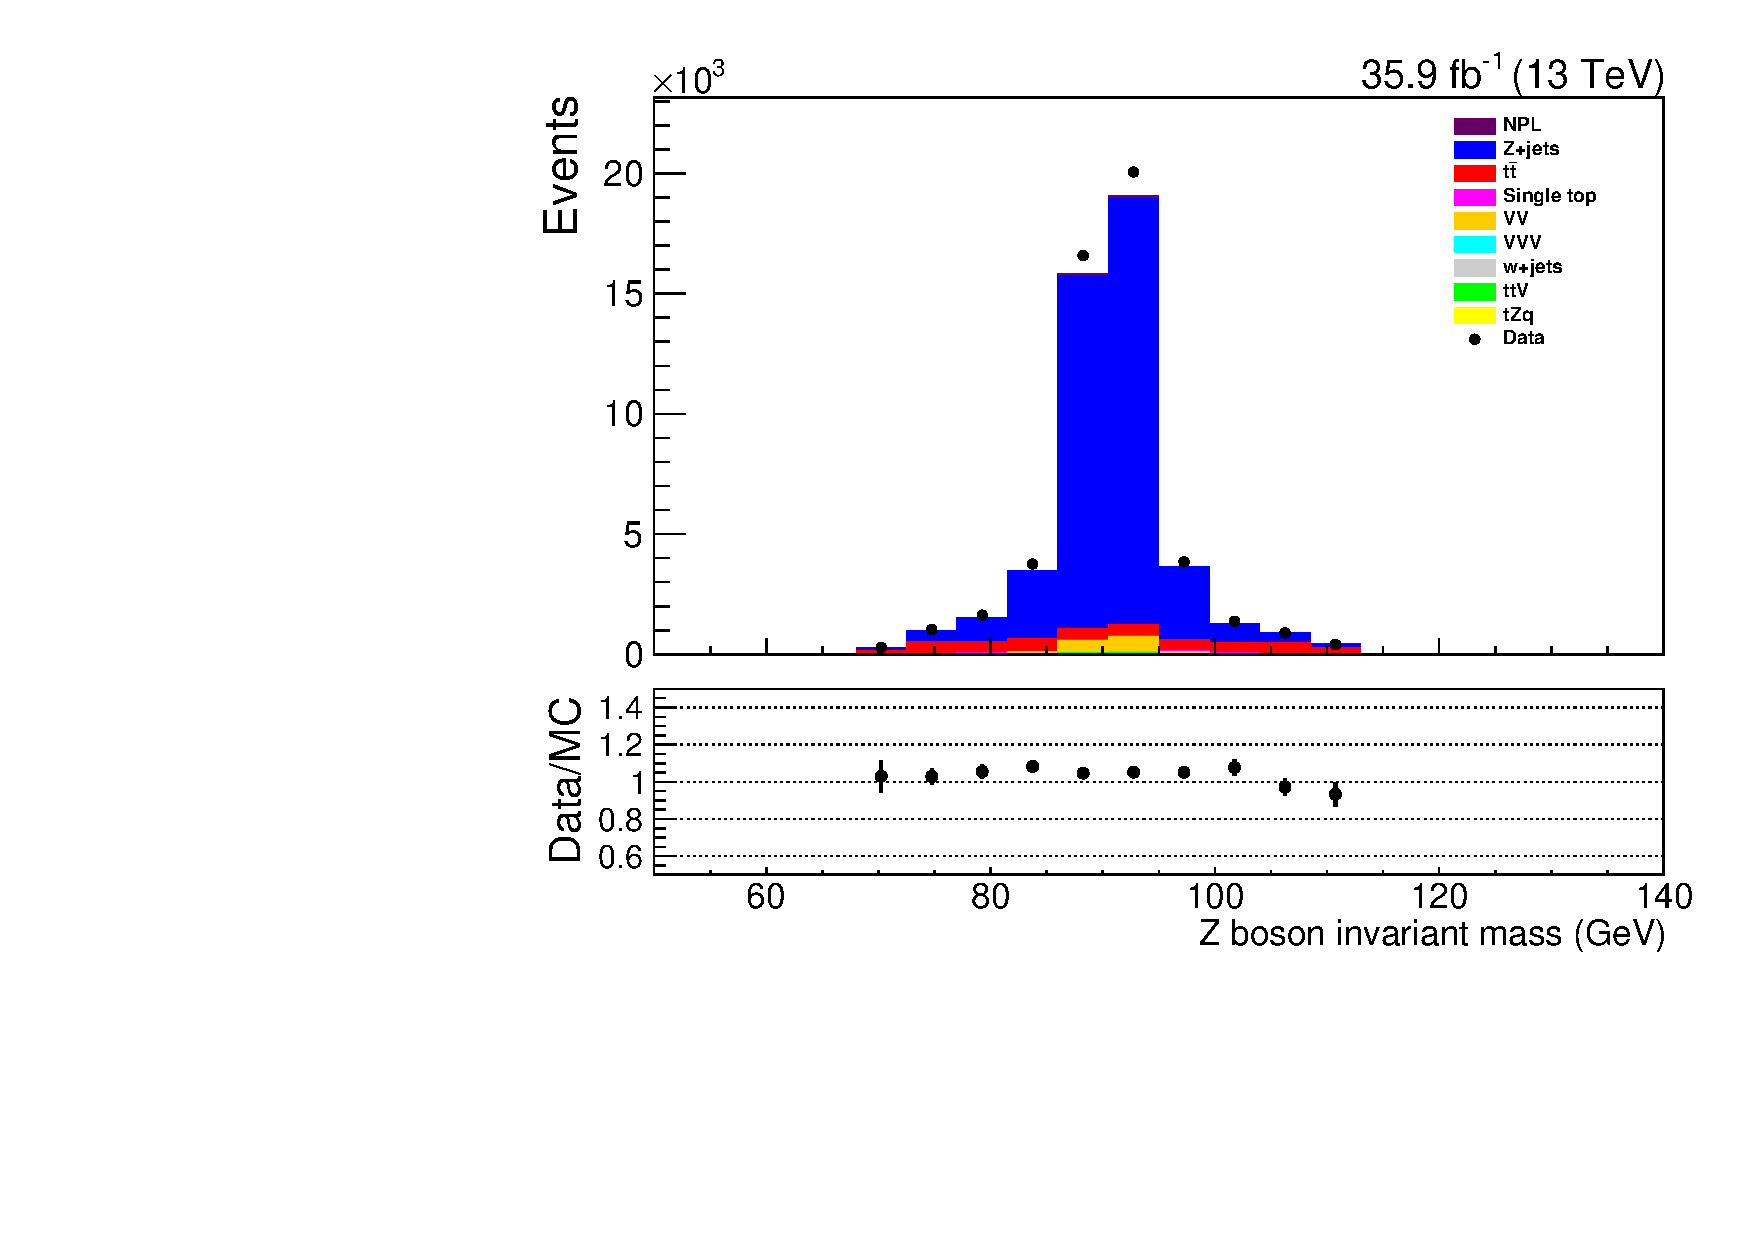
\includegraphics[width=0.47\textwidth]{figs/background-estimation/plots/unblinded/prompt_ee_ttbarInc/zPairMass_NPL_ee_jetSel_ee.pdf}
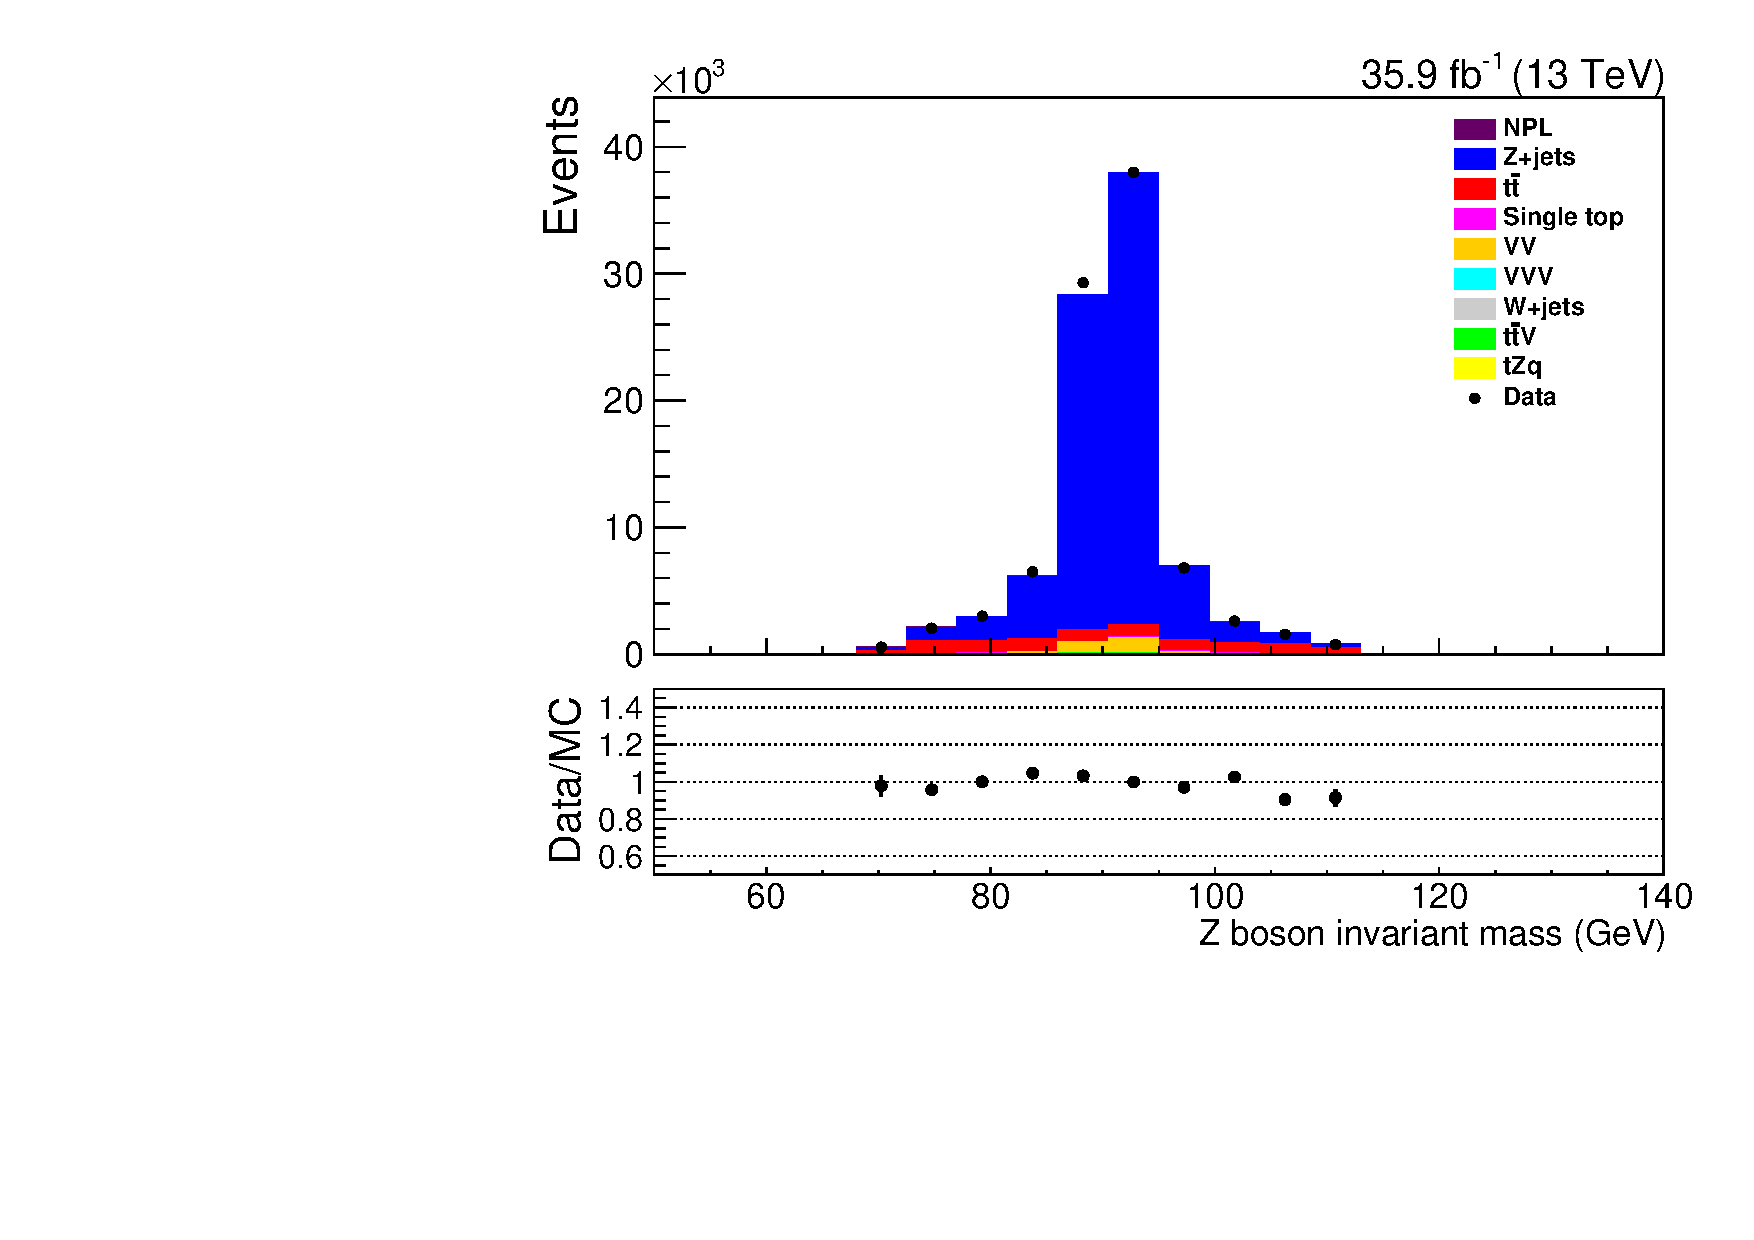
\includegraphics[width=0.47\textwidth]{figs/background-estimation/plots/unblinded/prompt_mumu_ttbarInc/zPairMass_NPL_mumu_jetSel_mumu.pdf}
\\
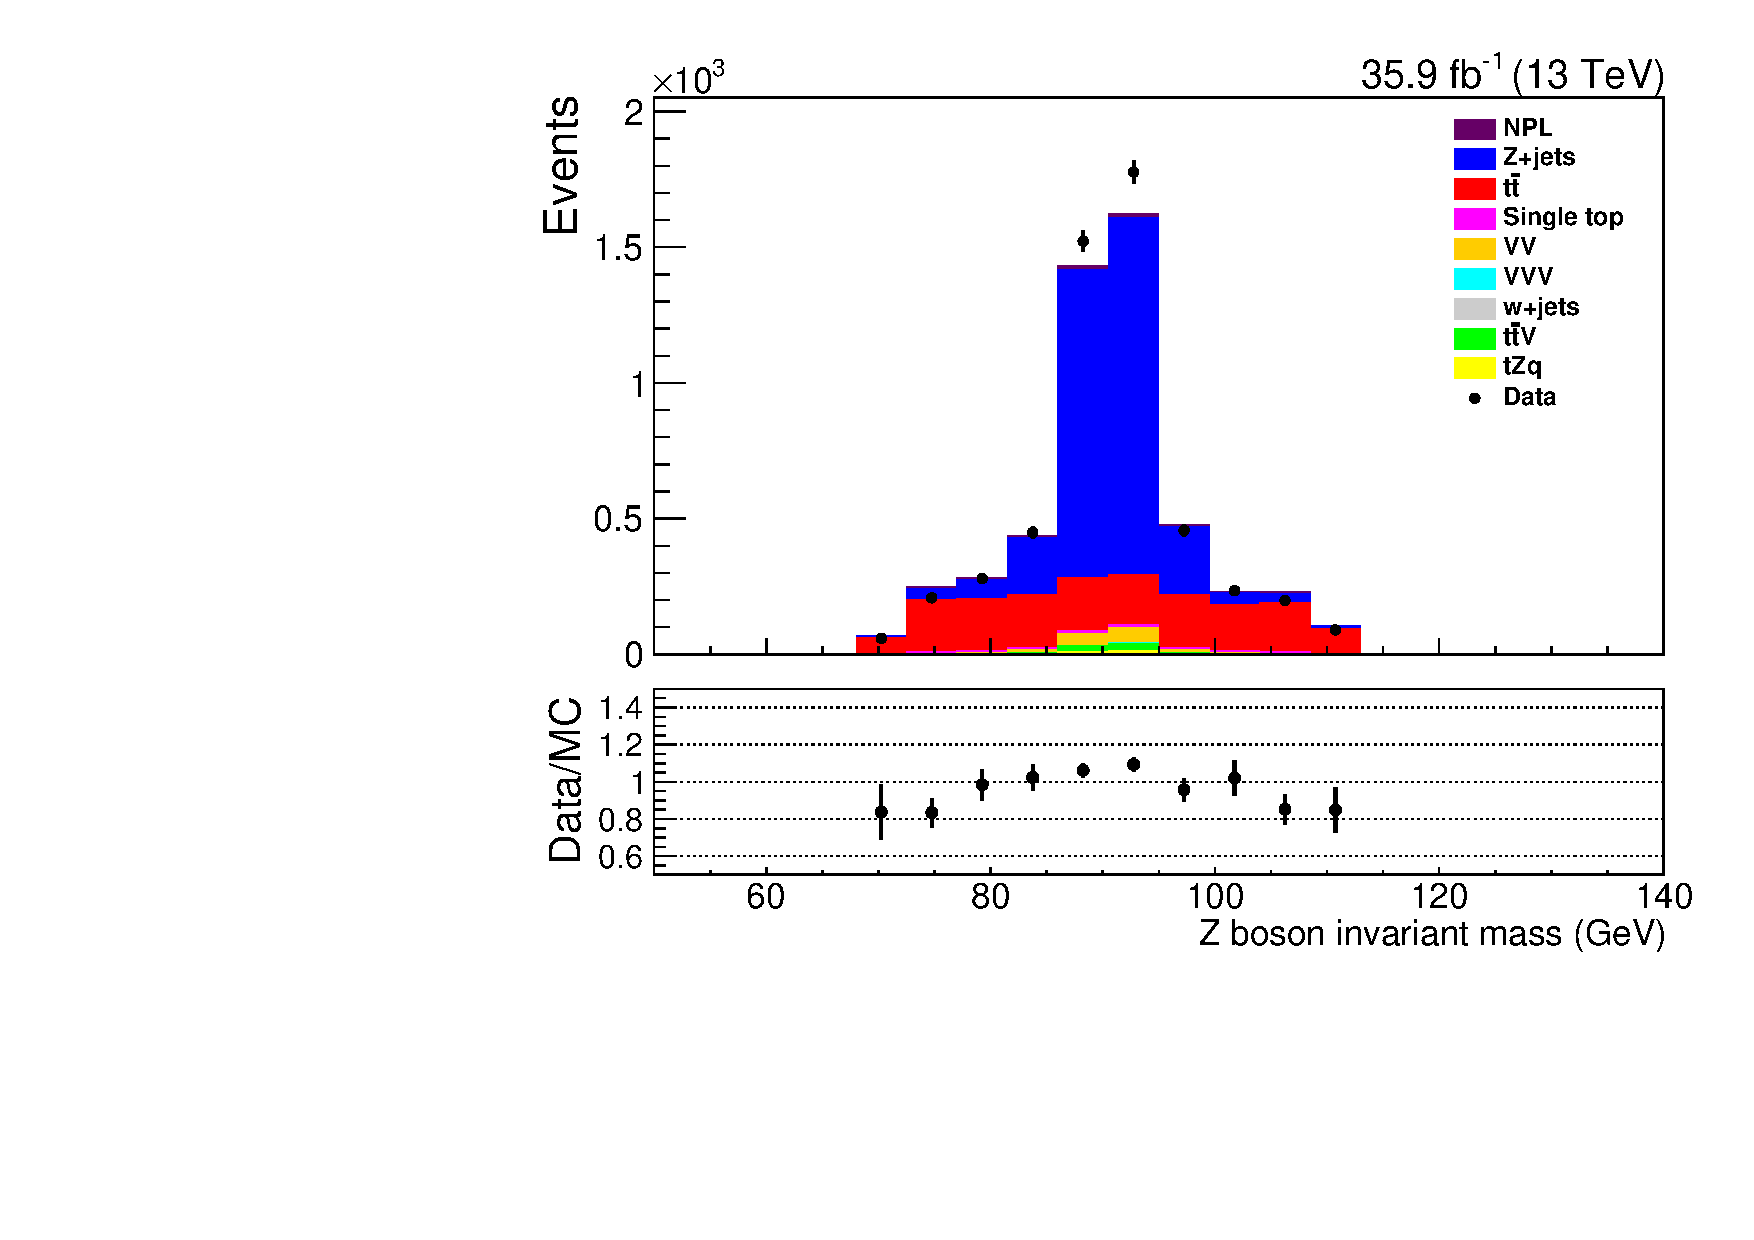
\includegraphics[width=0.47\textwidth]{figs/background-estimation/plots/unblinded/prompt_ee_ttbarInc/zPairMass_NPL_ee_wMass_ee.pdf}
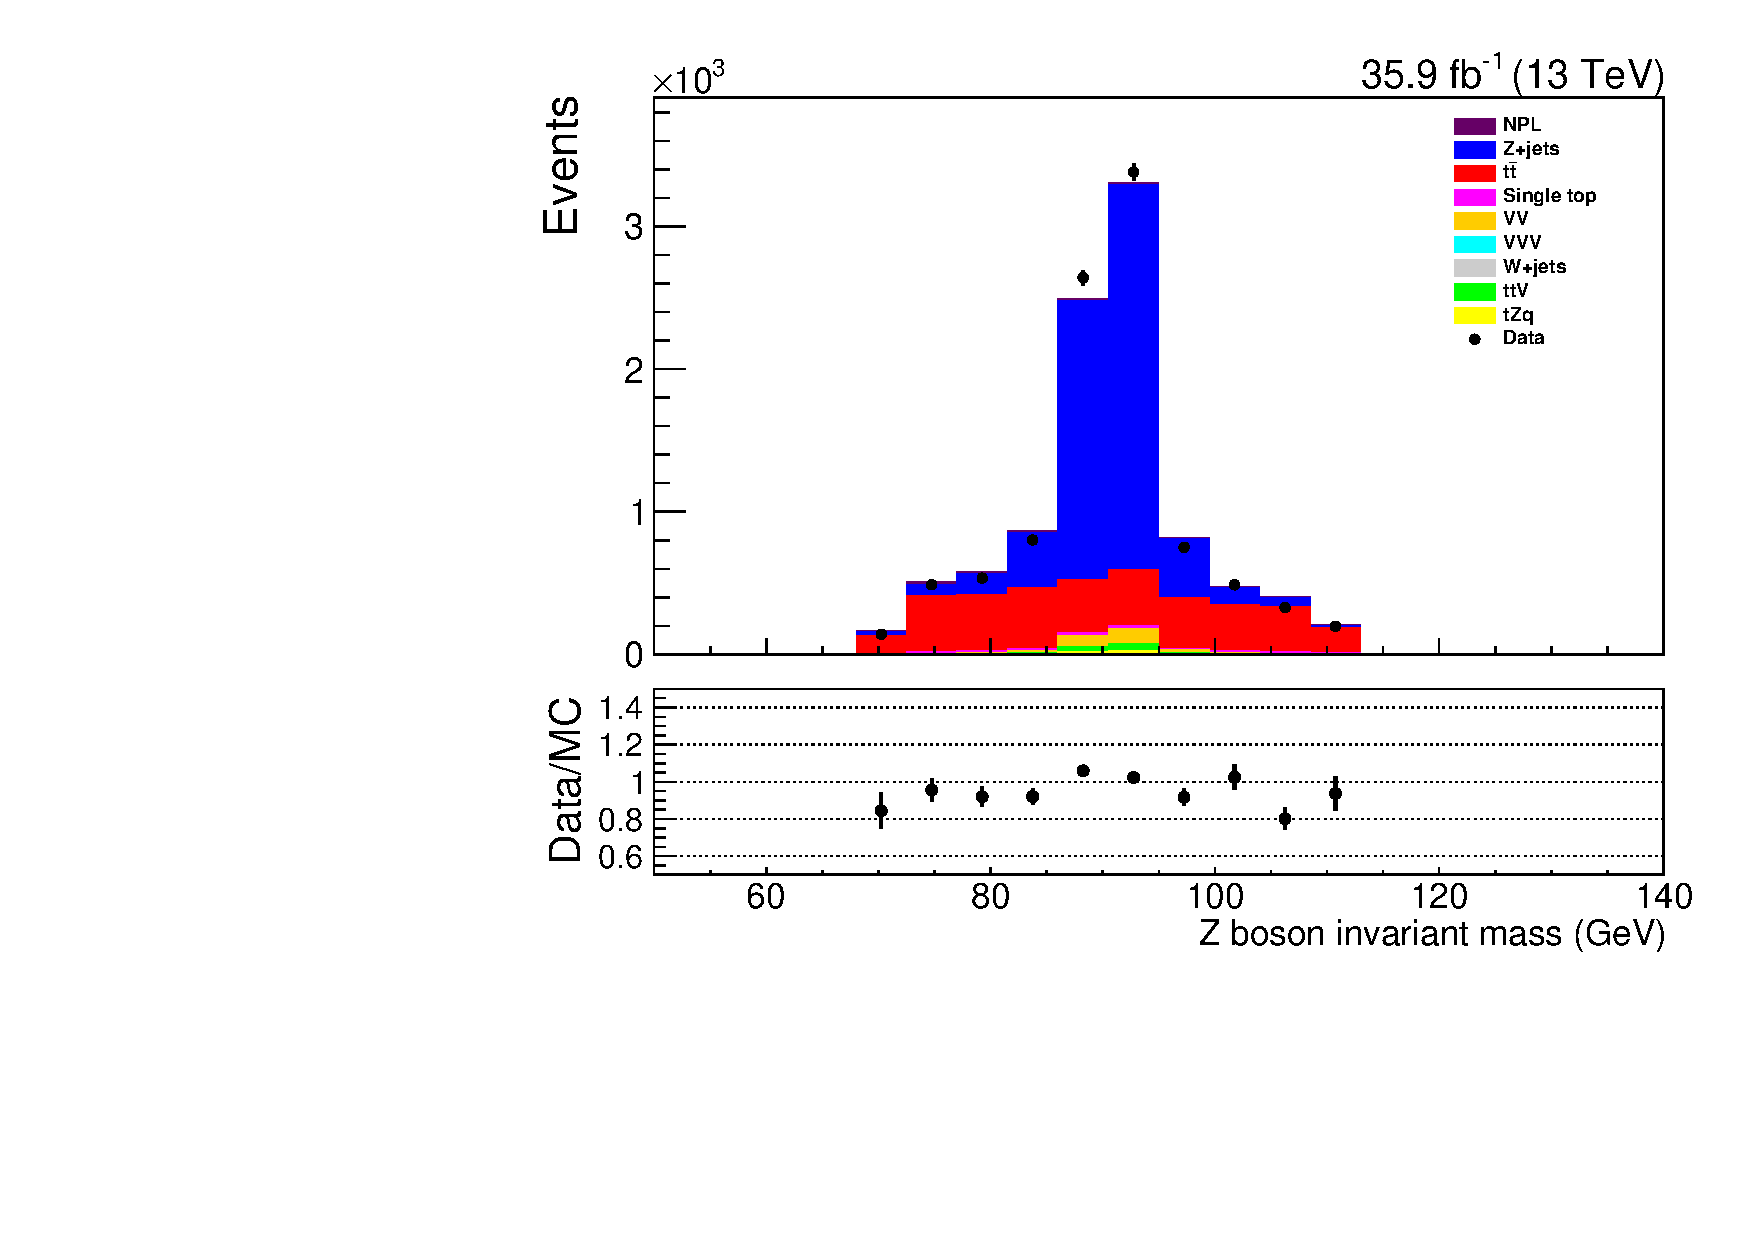
\includegraphics[width=0.47\textwidth]{figs/background-estimation/plots/unblinded/prompt_mumu_ttbarInc/zPairMass_NPL_mumu_wMass_mumu.pdf}
\caption{
The reconstructed Z boson mass following only the lepton selection criteria and simulation corrections (top), the jet selection criteria (middle) and all of the signal region selection criteria (bottom).
}
\label{fig:SR_zBosonMass}
\end{figure}

\begin{figure}[h]
\centering
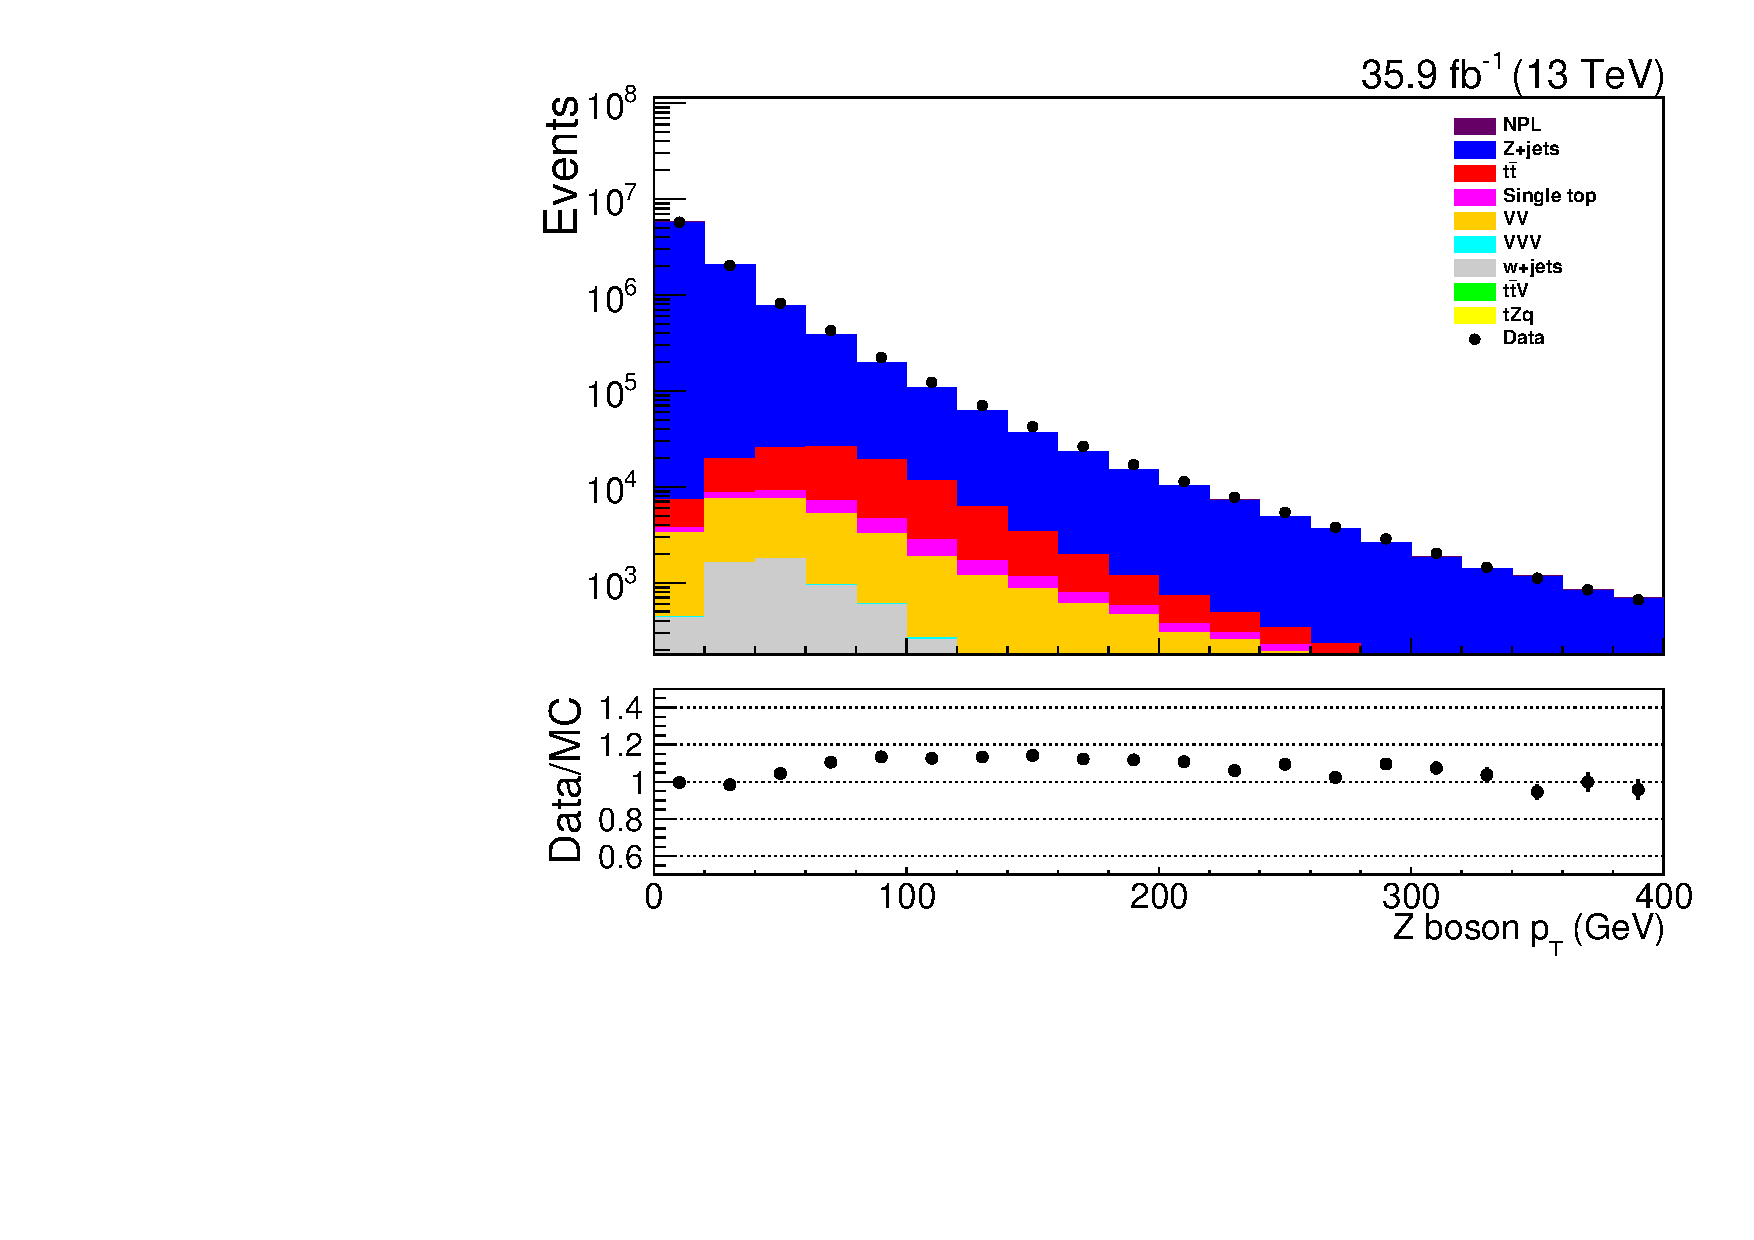
\includegraphics[width=0.47\textwidth]{figs/background-estimation/plots/unblinded/prompt_ee_ttbarInc/zPairPt_NPL_ee_lepSel_ee_log.pdf}
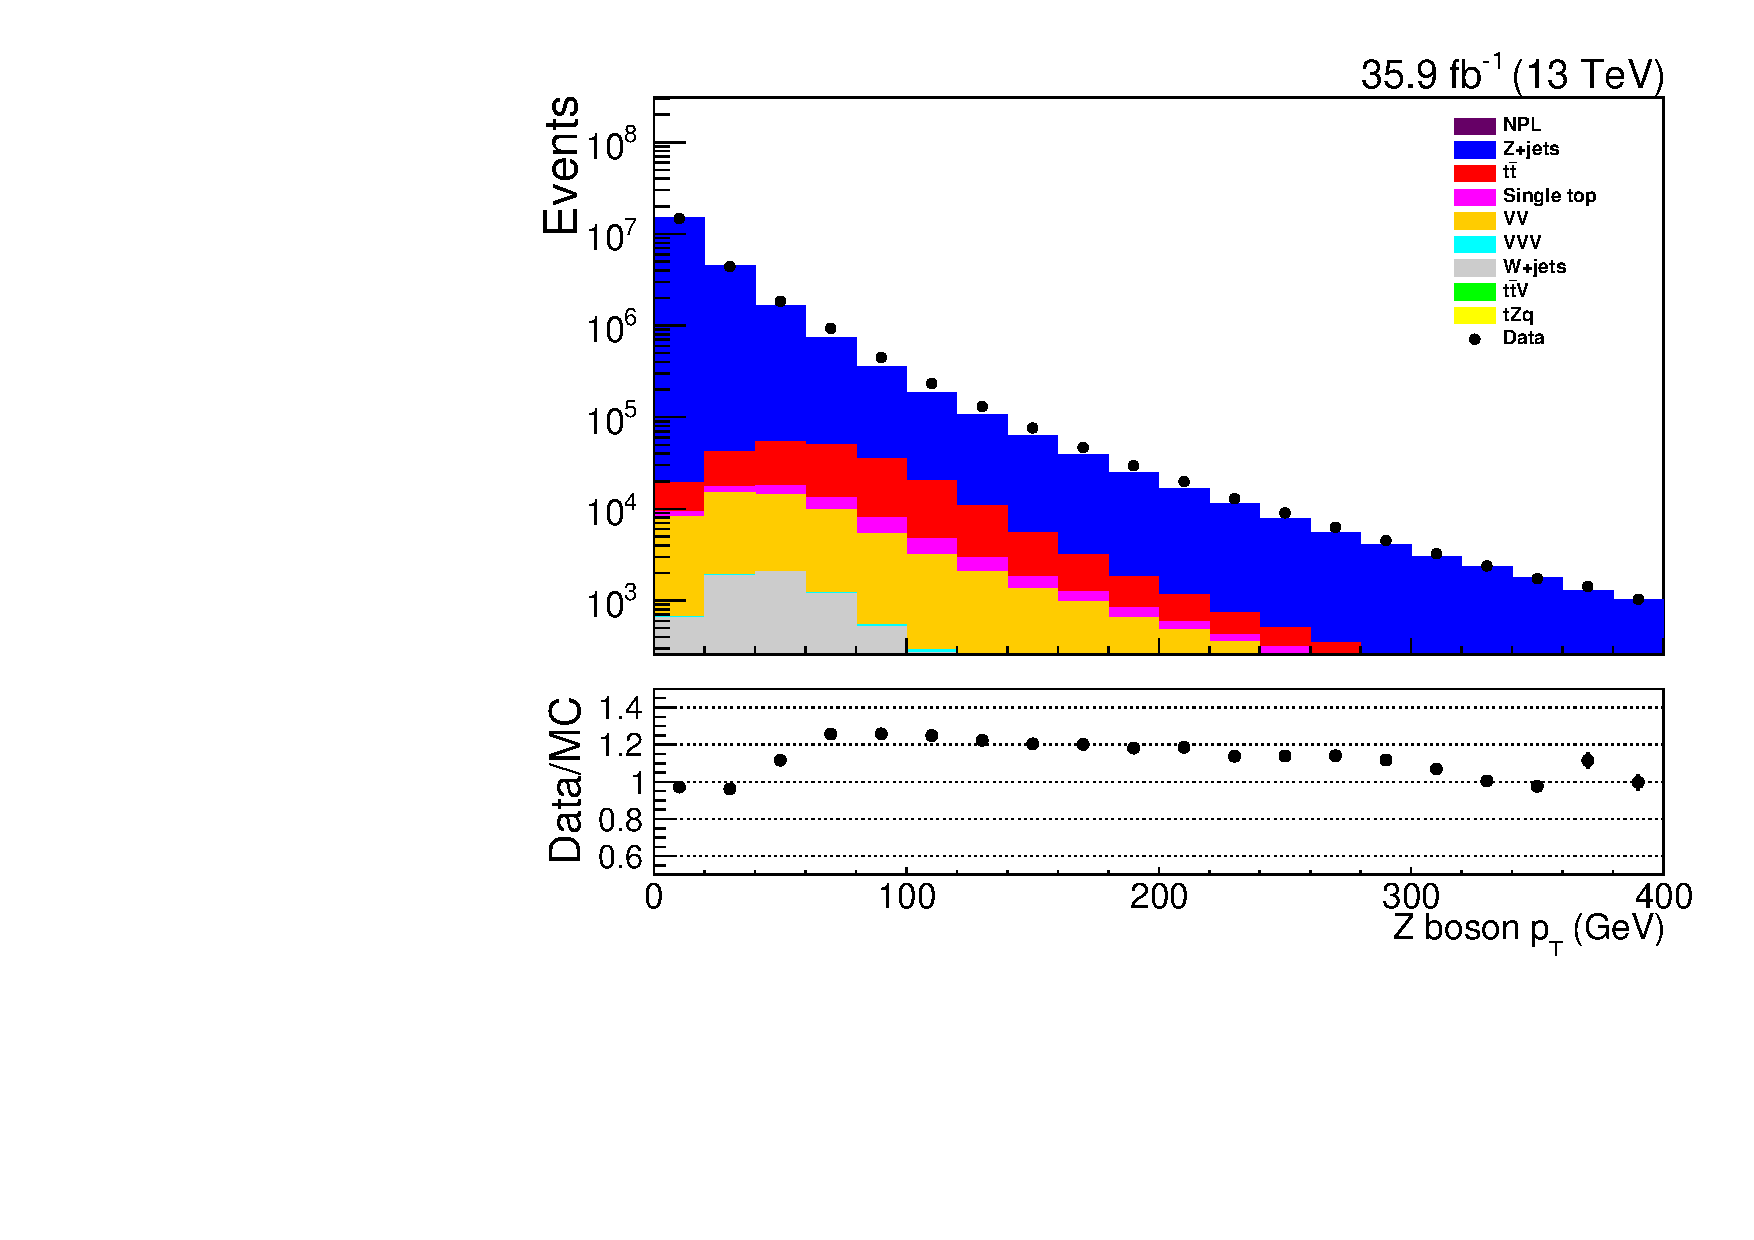
\includegraphics[width=0.47\textwidth]{figs/background-estimation/plots/unblinded/prompt_mumu_ttbarInc/zPairPt_NPL_mumu_lepSel_mumu_log.pdf}
\\
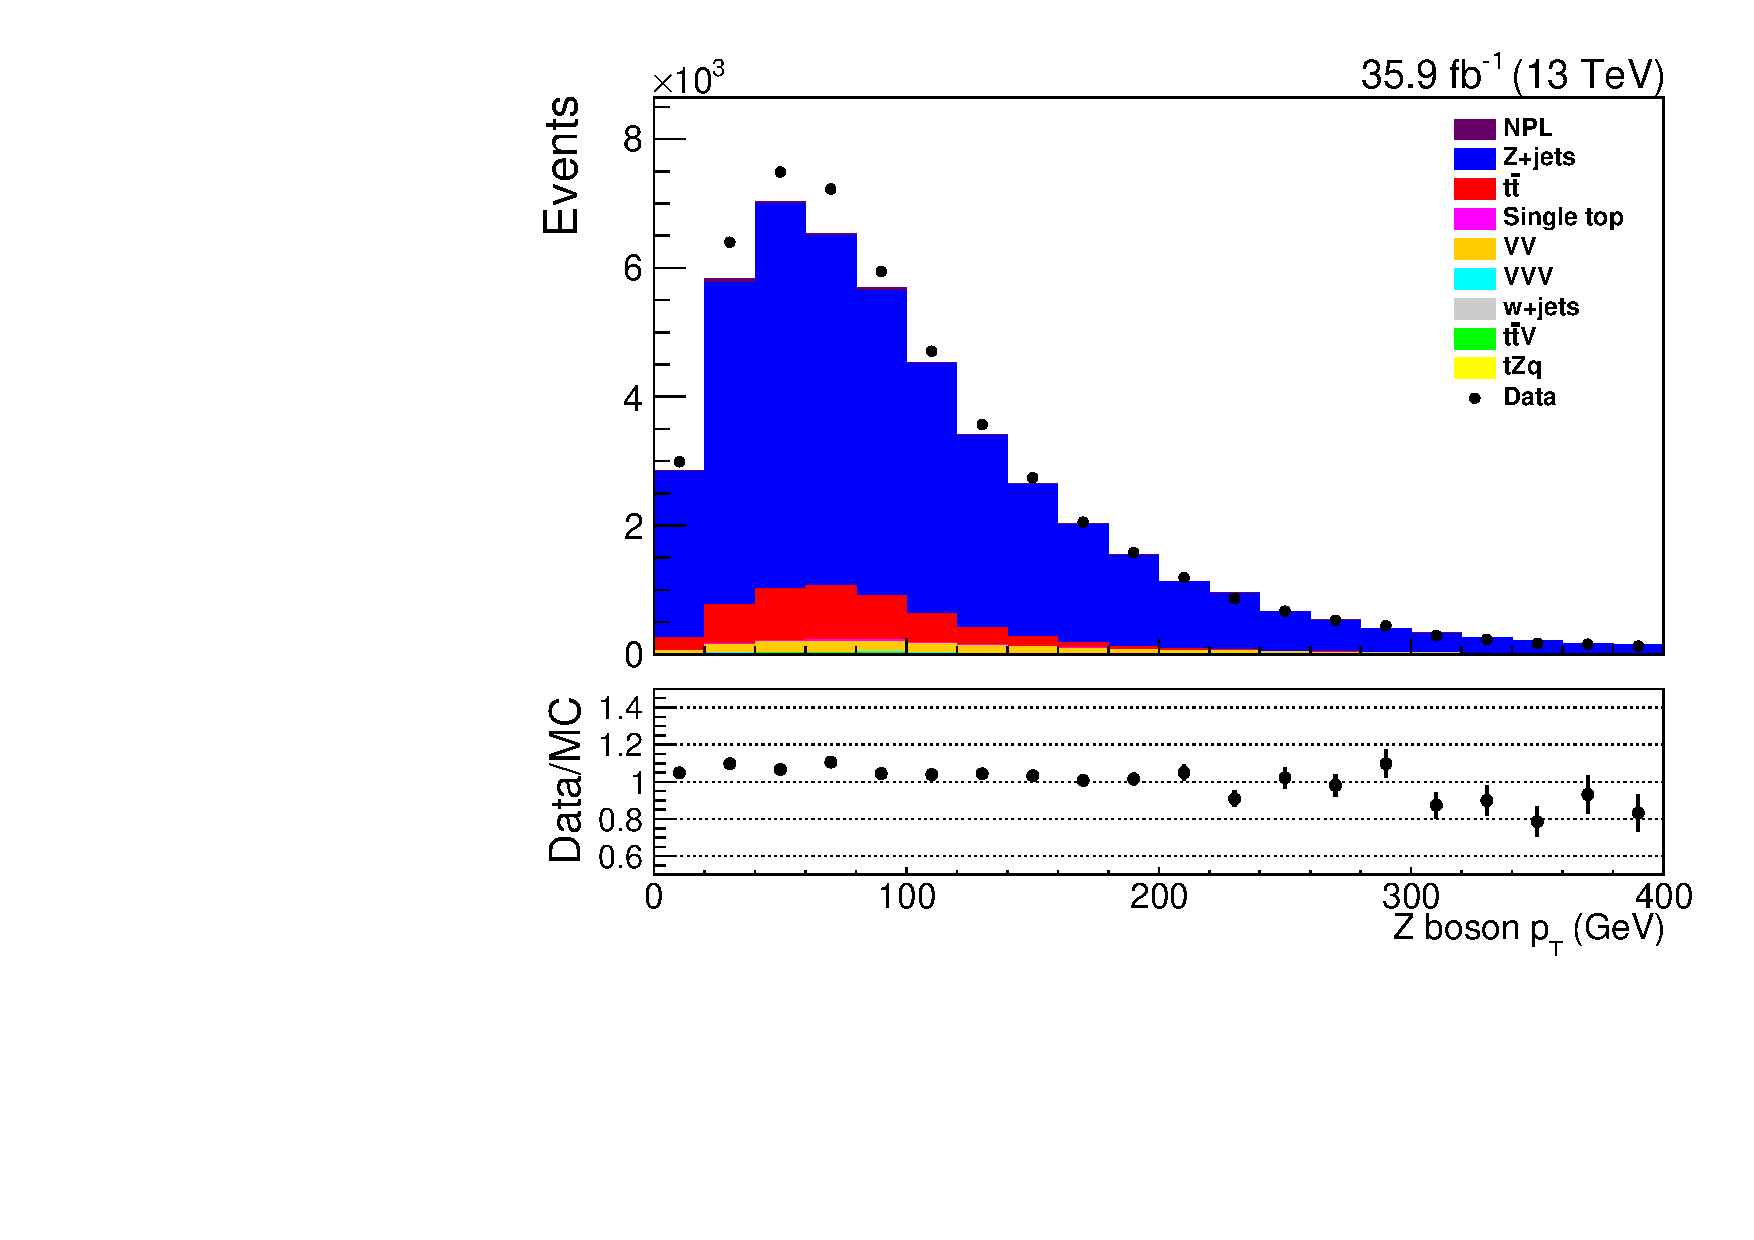
\includegraphics[width=0.47\textwidth]{figs/background-estimation/plots/unblinded/prompt_ee_ttbarInc/zPairPt_NPL_ee_jetSel_ee.pdf}
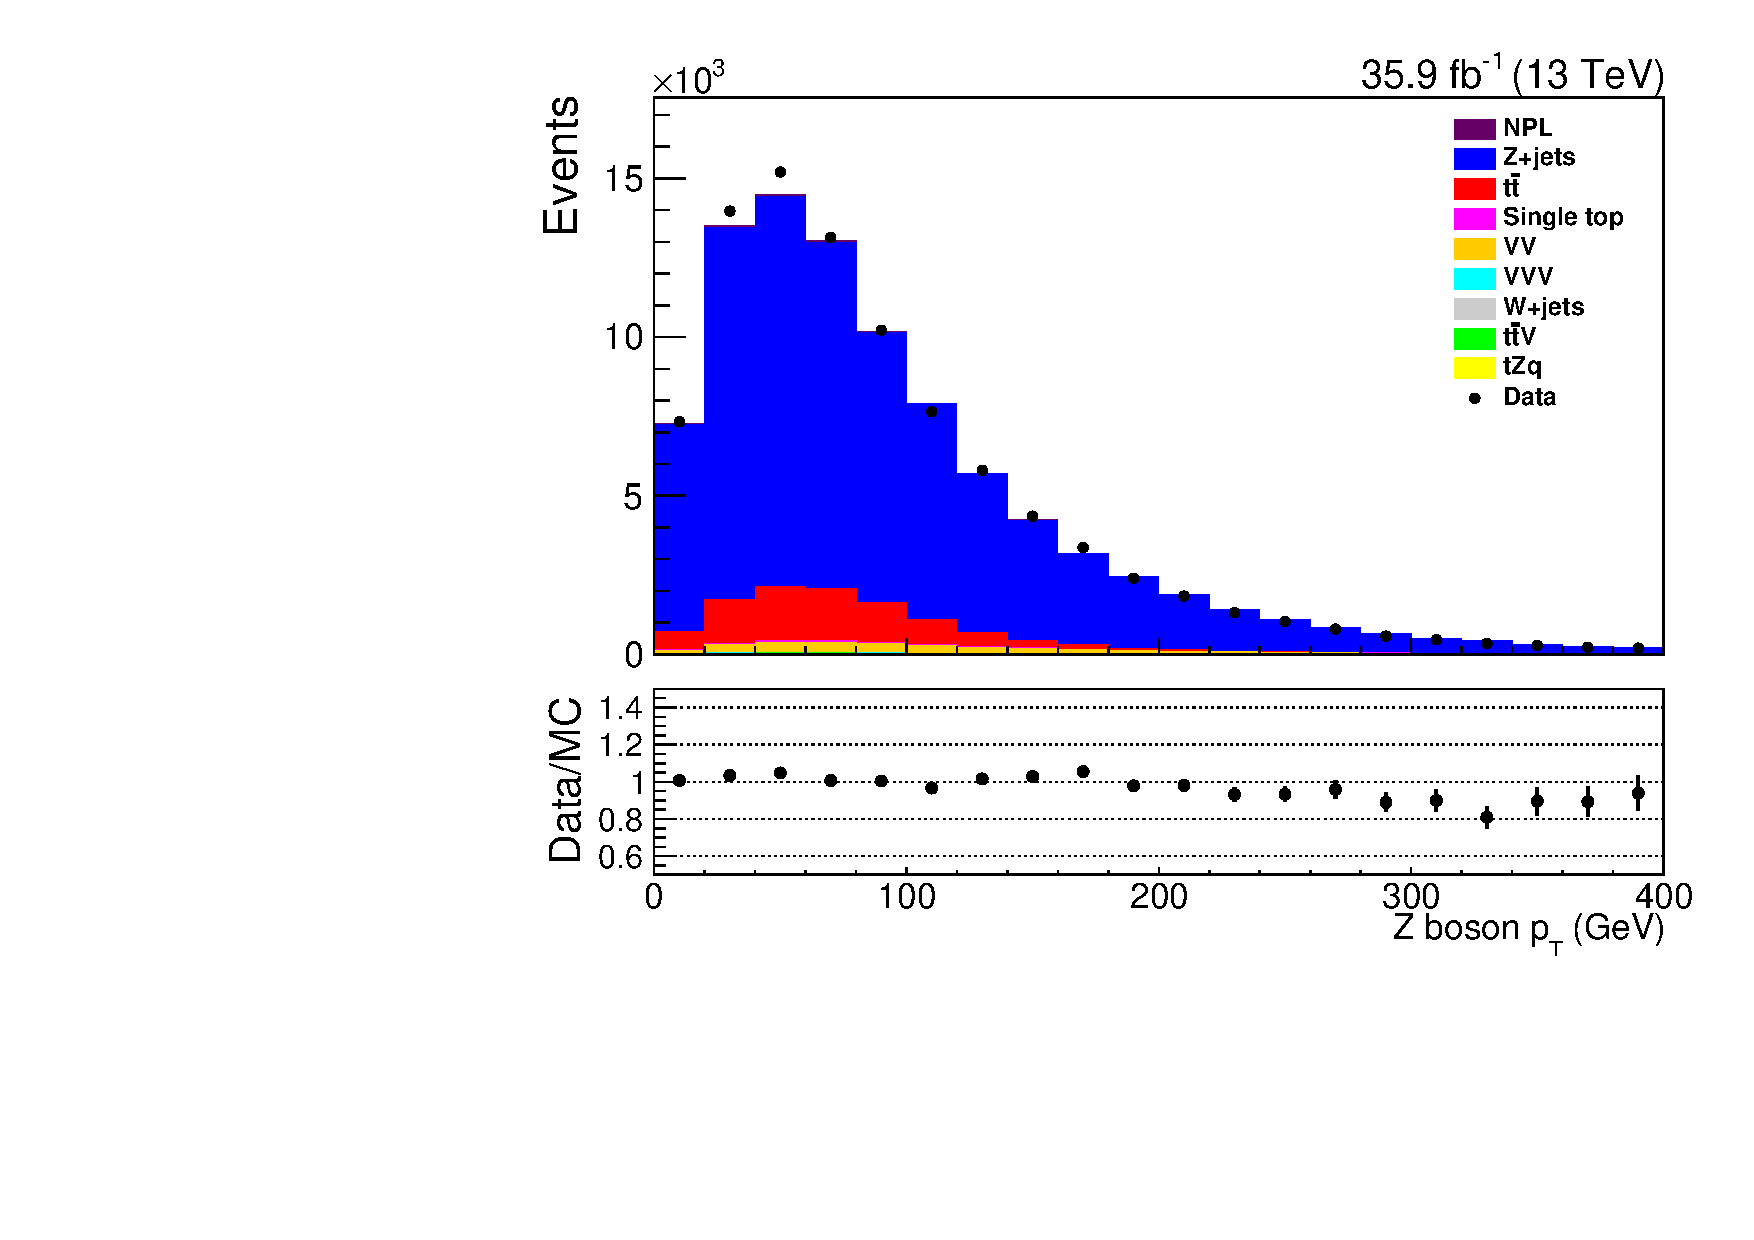
\includegraphics[width=0.47\textwidth]{figs/background-estimation/plots/unblinded/prompt_mumu_ttbarInc/zPairPt_NPL_mumu_jetSel_mumu.pdf}
\\
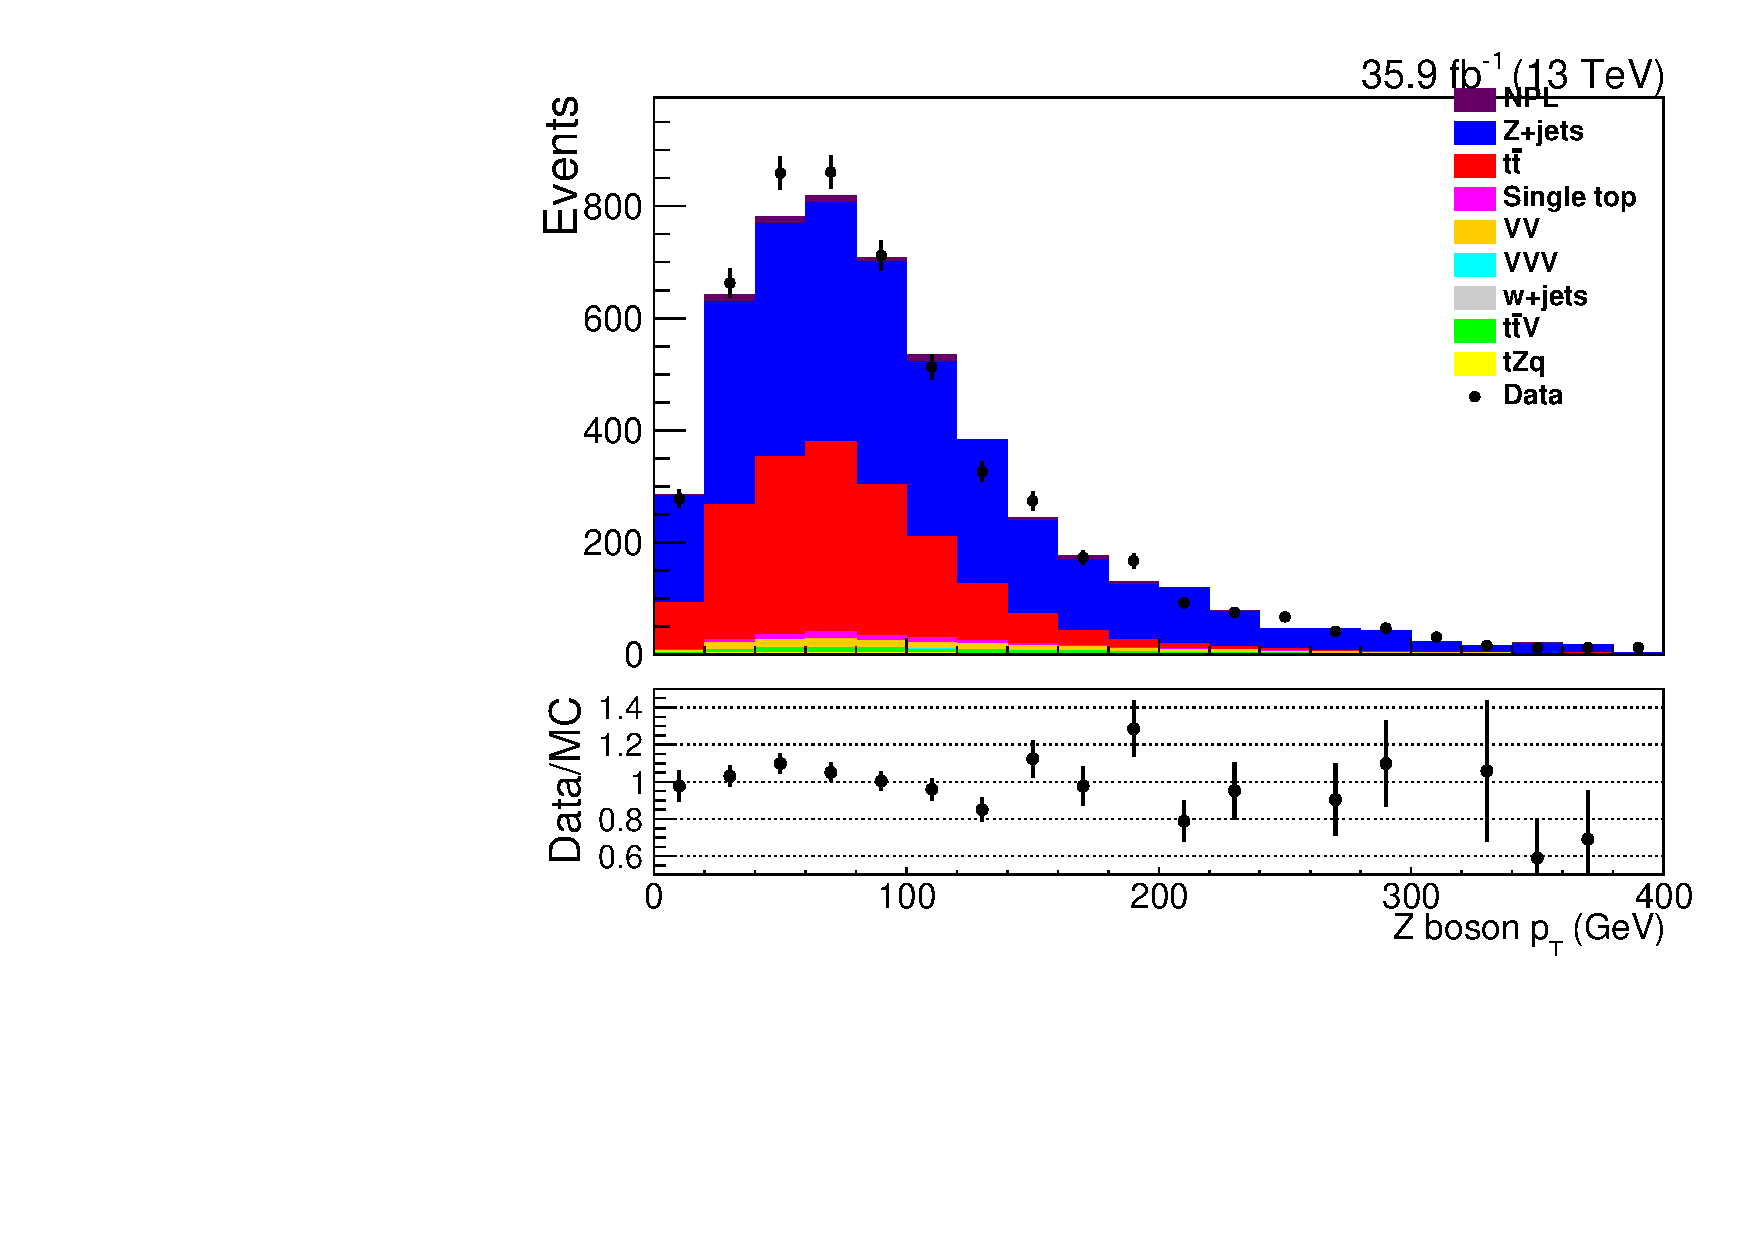
\includegraphics[width=0.47\textwidth]{figs/background-estimation/plots/unblinded/prompt_ee_ttbarInc/zPairPt_NPL_ee_wMass_ee.pdf}
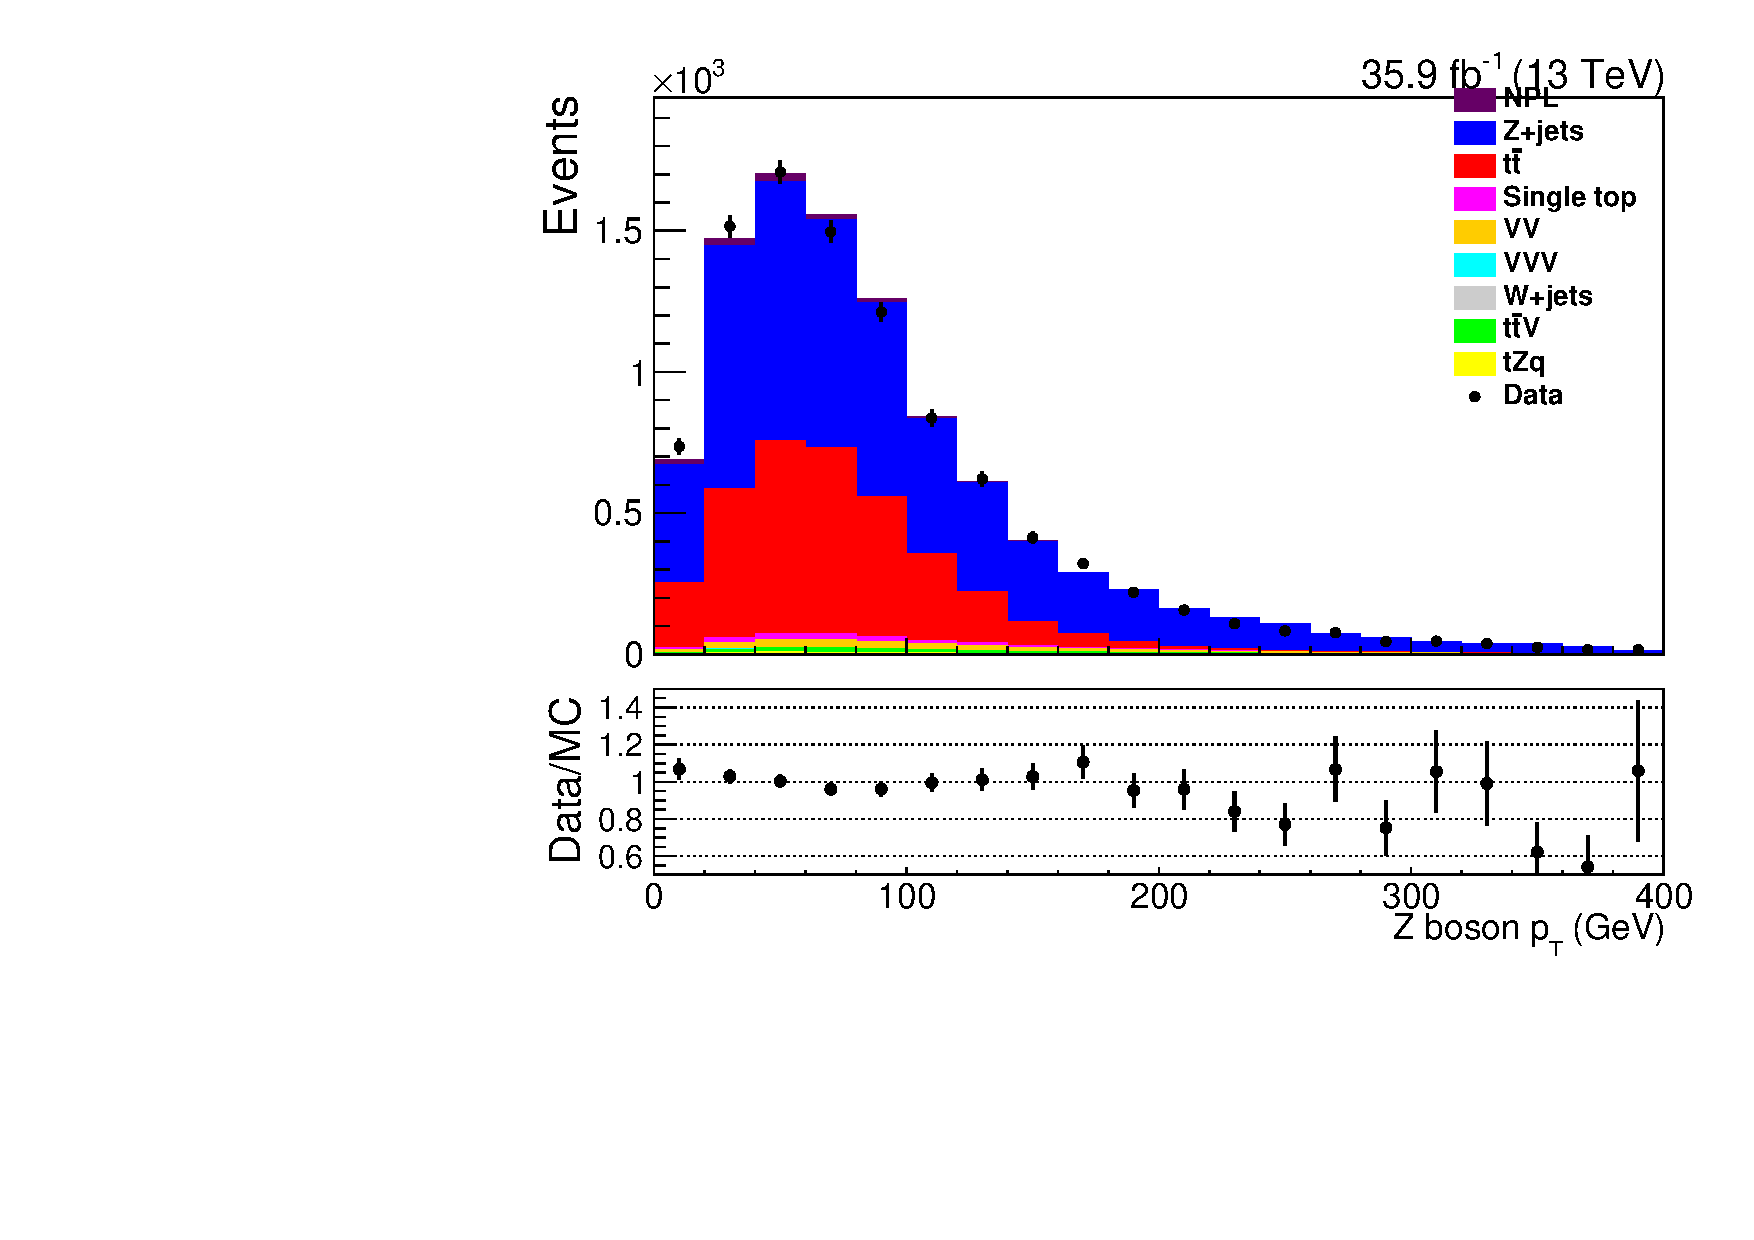
\includegraphics[width=0.47\textwidth]{figs/background-estimation/plots/unblinded/prompt_mumu_ttbarInc/zPairPt_NPL_mumu_wMass_mumu.pdf}
\caption{
The reconstructed Z boson mass \pT following only the lepton selection criteria and simulation corrections (top), the jet selection criteria (middle) and all of the signal region selection criteria (bottom).
}
\label{fig:SR_zBosonPt}
\end{figure}

\clearpage
\newpage	

\section{Z+jets Control Region}\label{appSec:signalRegionPlots}

\clearpage
\newpage
\section{\ttbar Control Region}\label{appSec:signalRegionPlots}

\begin{figure}[!h]
\centering
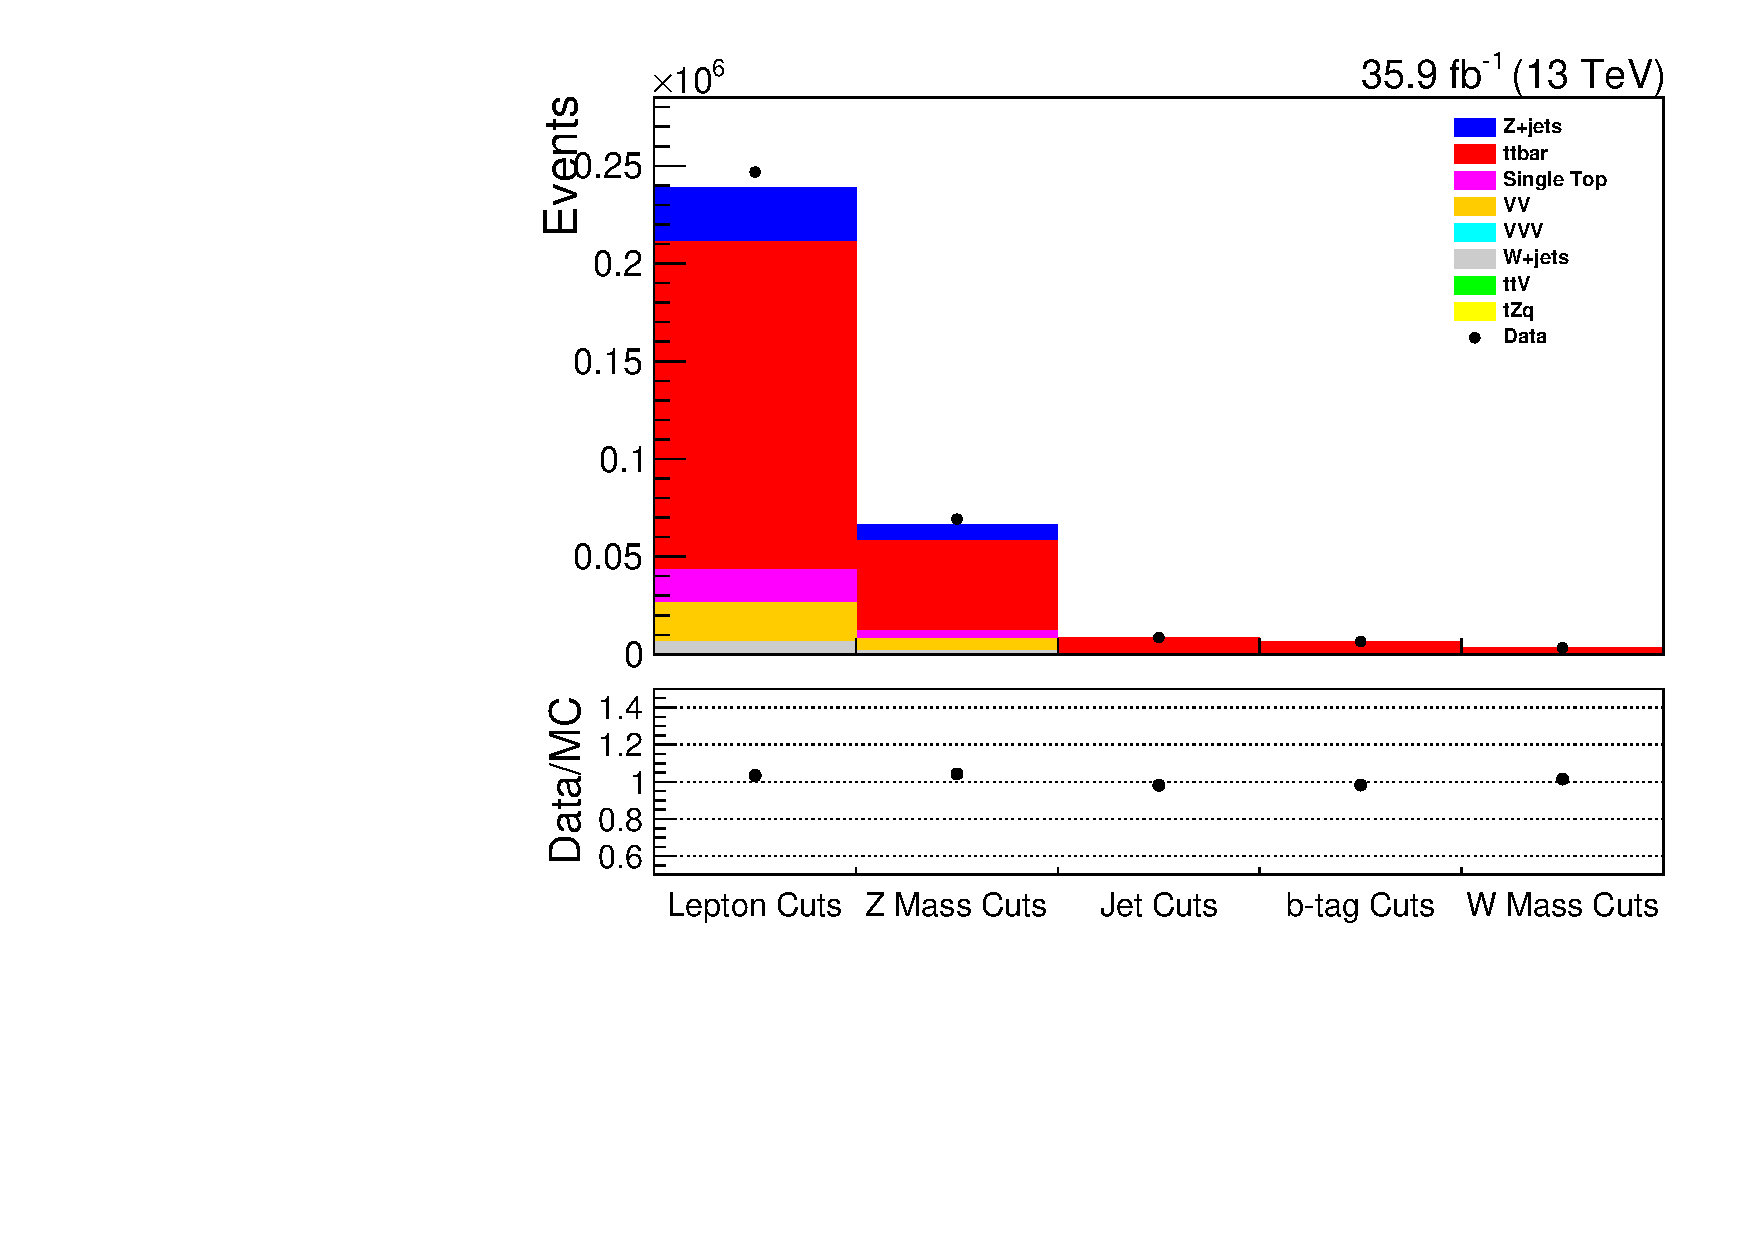
\includegraphics[width=0.97\textwidth]{figs/background-estimation/plots/unblinded/ttbar_control/cutFlow_log.pdf}
\caption{
The overall event yield for data and simulation at each stage of applying the signal region selection criteria and simulation corrections.
}
\label{fig:ttbar_cutFlow}
\end{figure}

\begin{figure}[h]
\centering
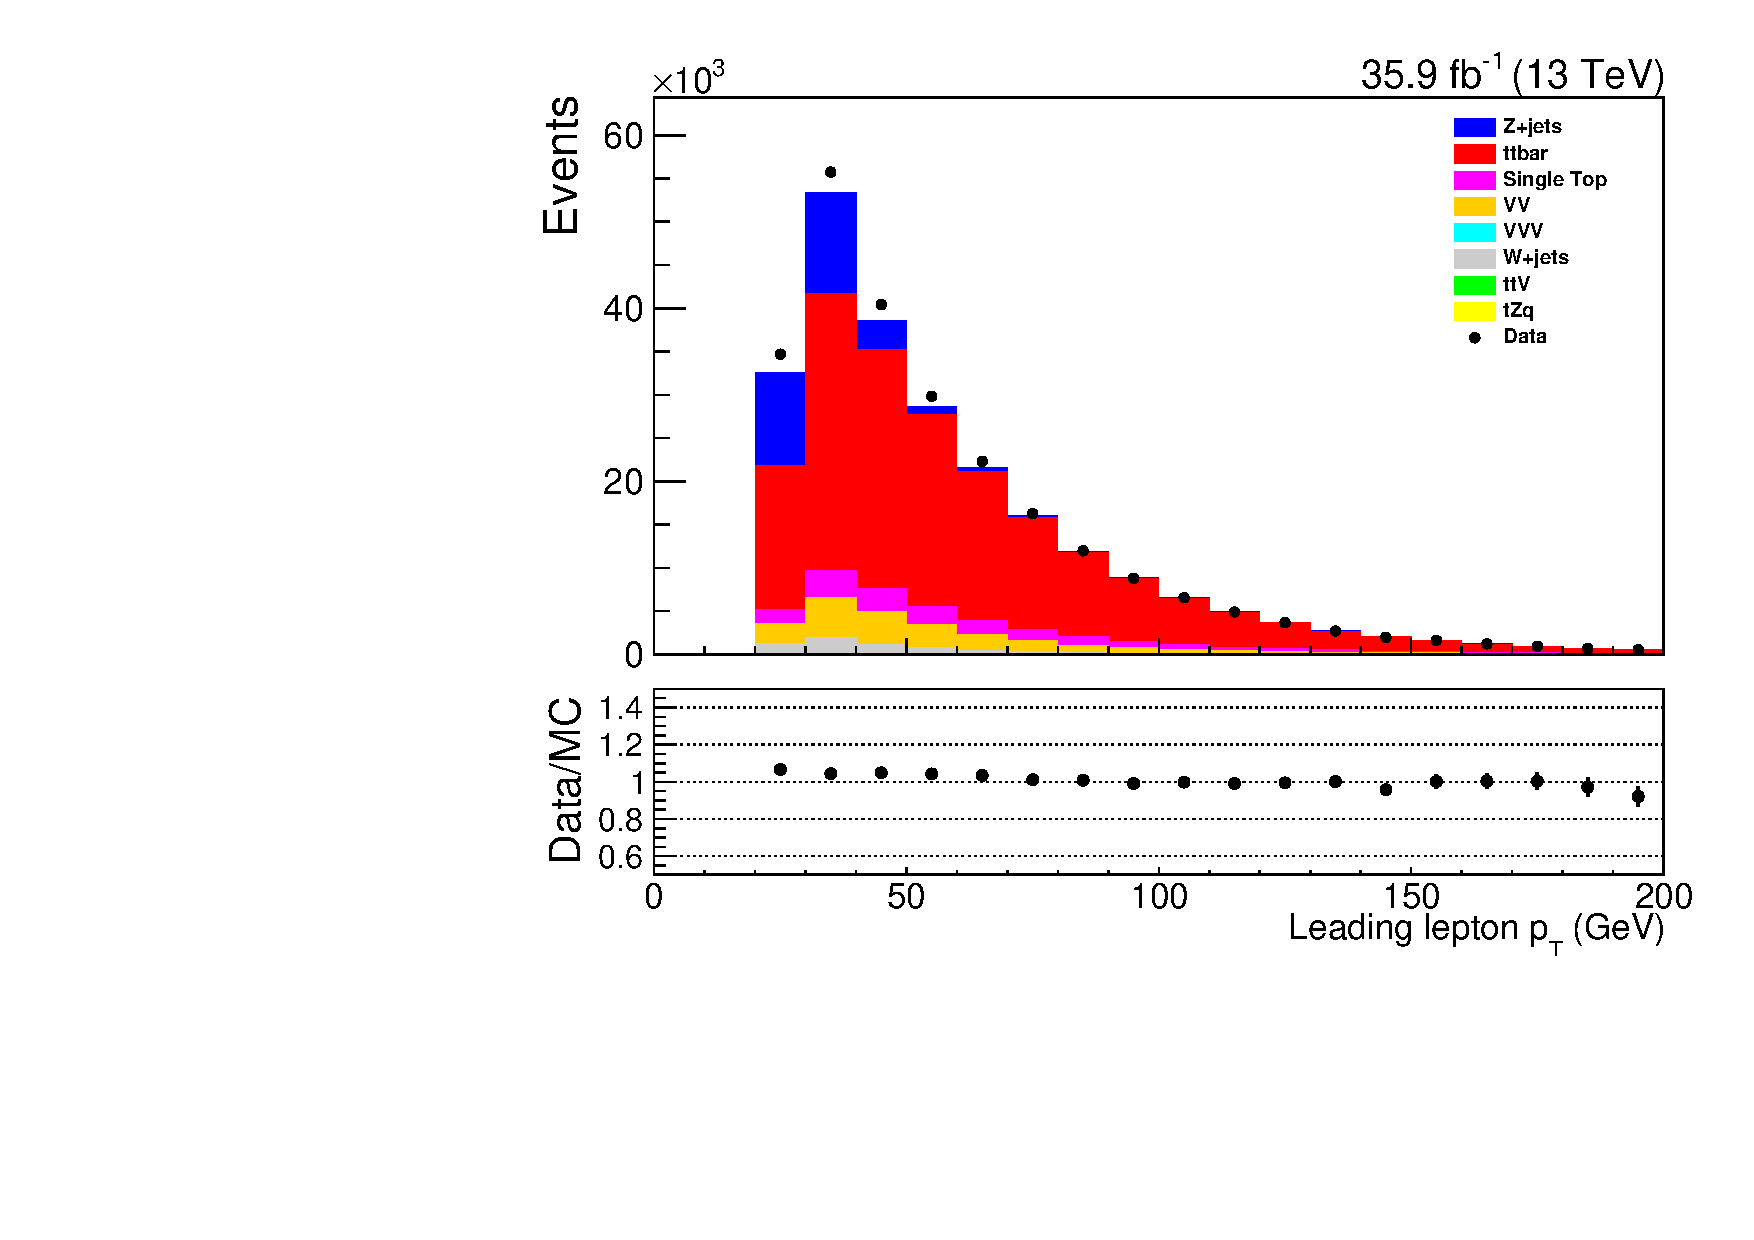
\includegraphics[width=0.47\textwidth]{figs/background-estimation/plots/unblinded/ttbar_control/lep1Pt_SingleTop_lepSel_emu_log.pdf}
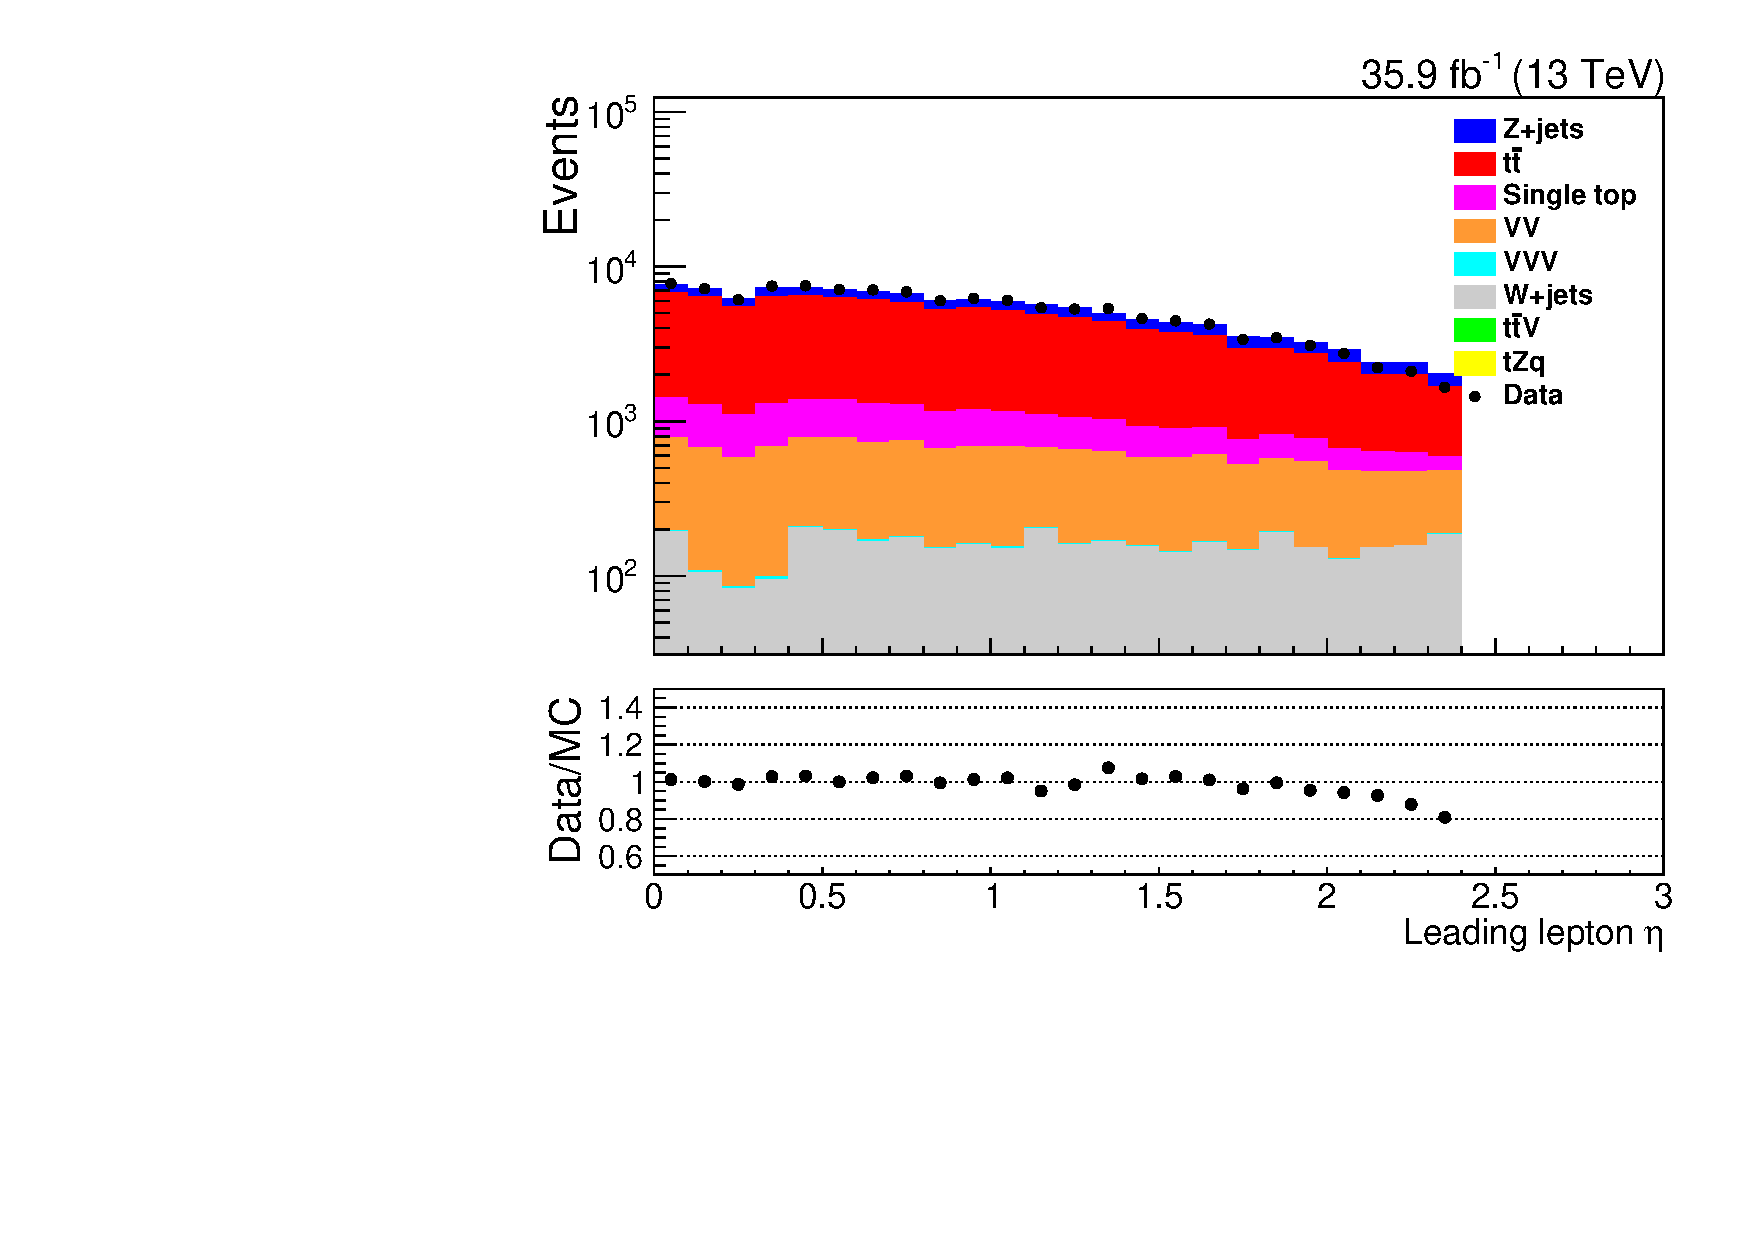
\includegraphics[width=0.47\textwidth]{figs/background-estimation/plots/unblinded/ttbar_control/lep1Eta_SingleTop_lepSel_emu_log.pdf}
\\
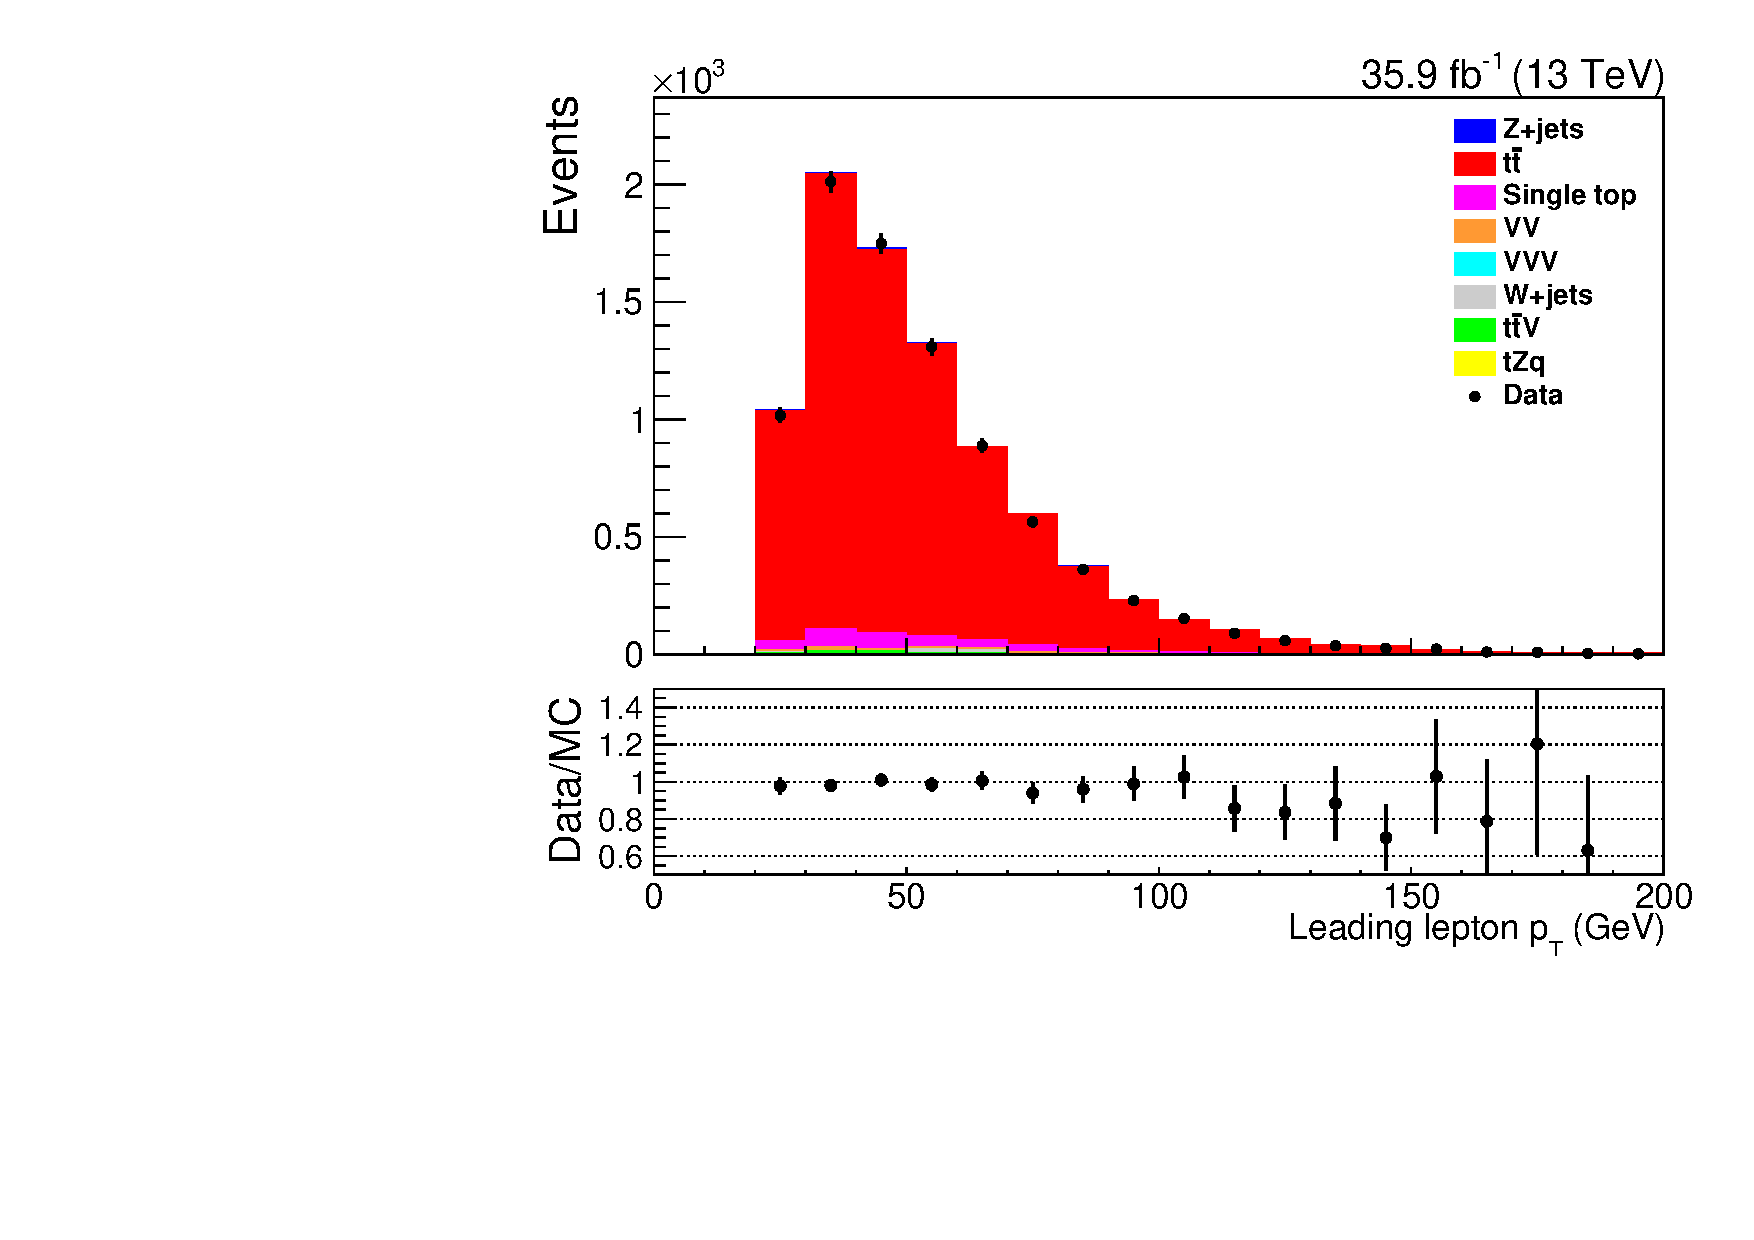
\includegraphics[width=0.47\textwidth]{figs/background-estimation/plots/unblinded/ttbar_control/lep1Pt_SingleTop_jetSel_emu.pdf}
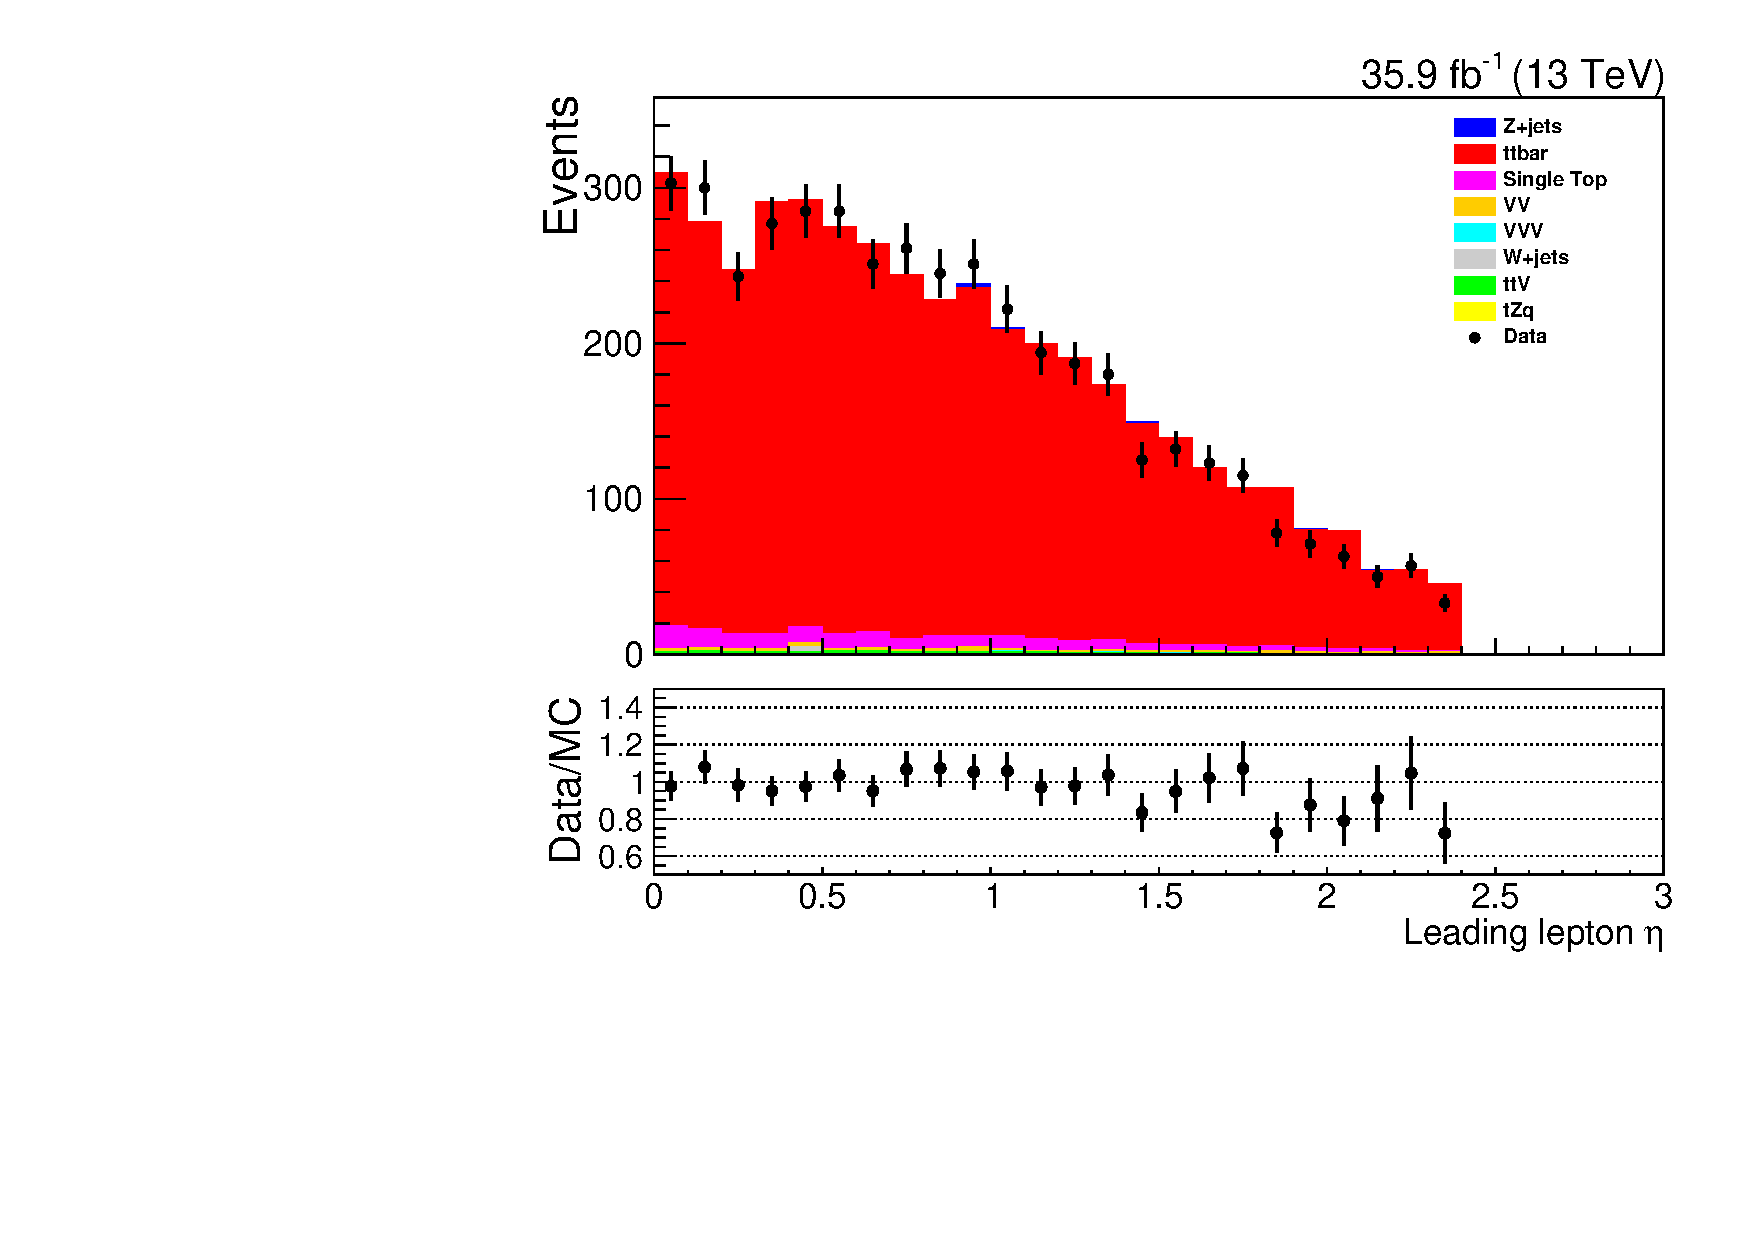
\includegraphics[width=0.47\textwidth]{figs/background-estimation/plots/unblinded/ttbar_control/lep1Eta_SingleTop_jetSel_emu.pdf}
\\
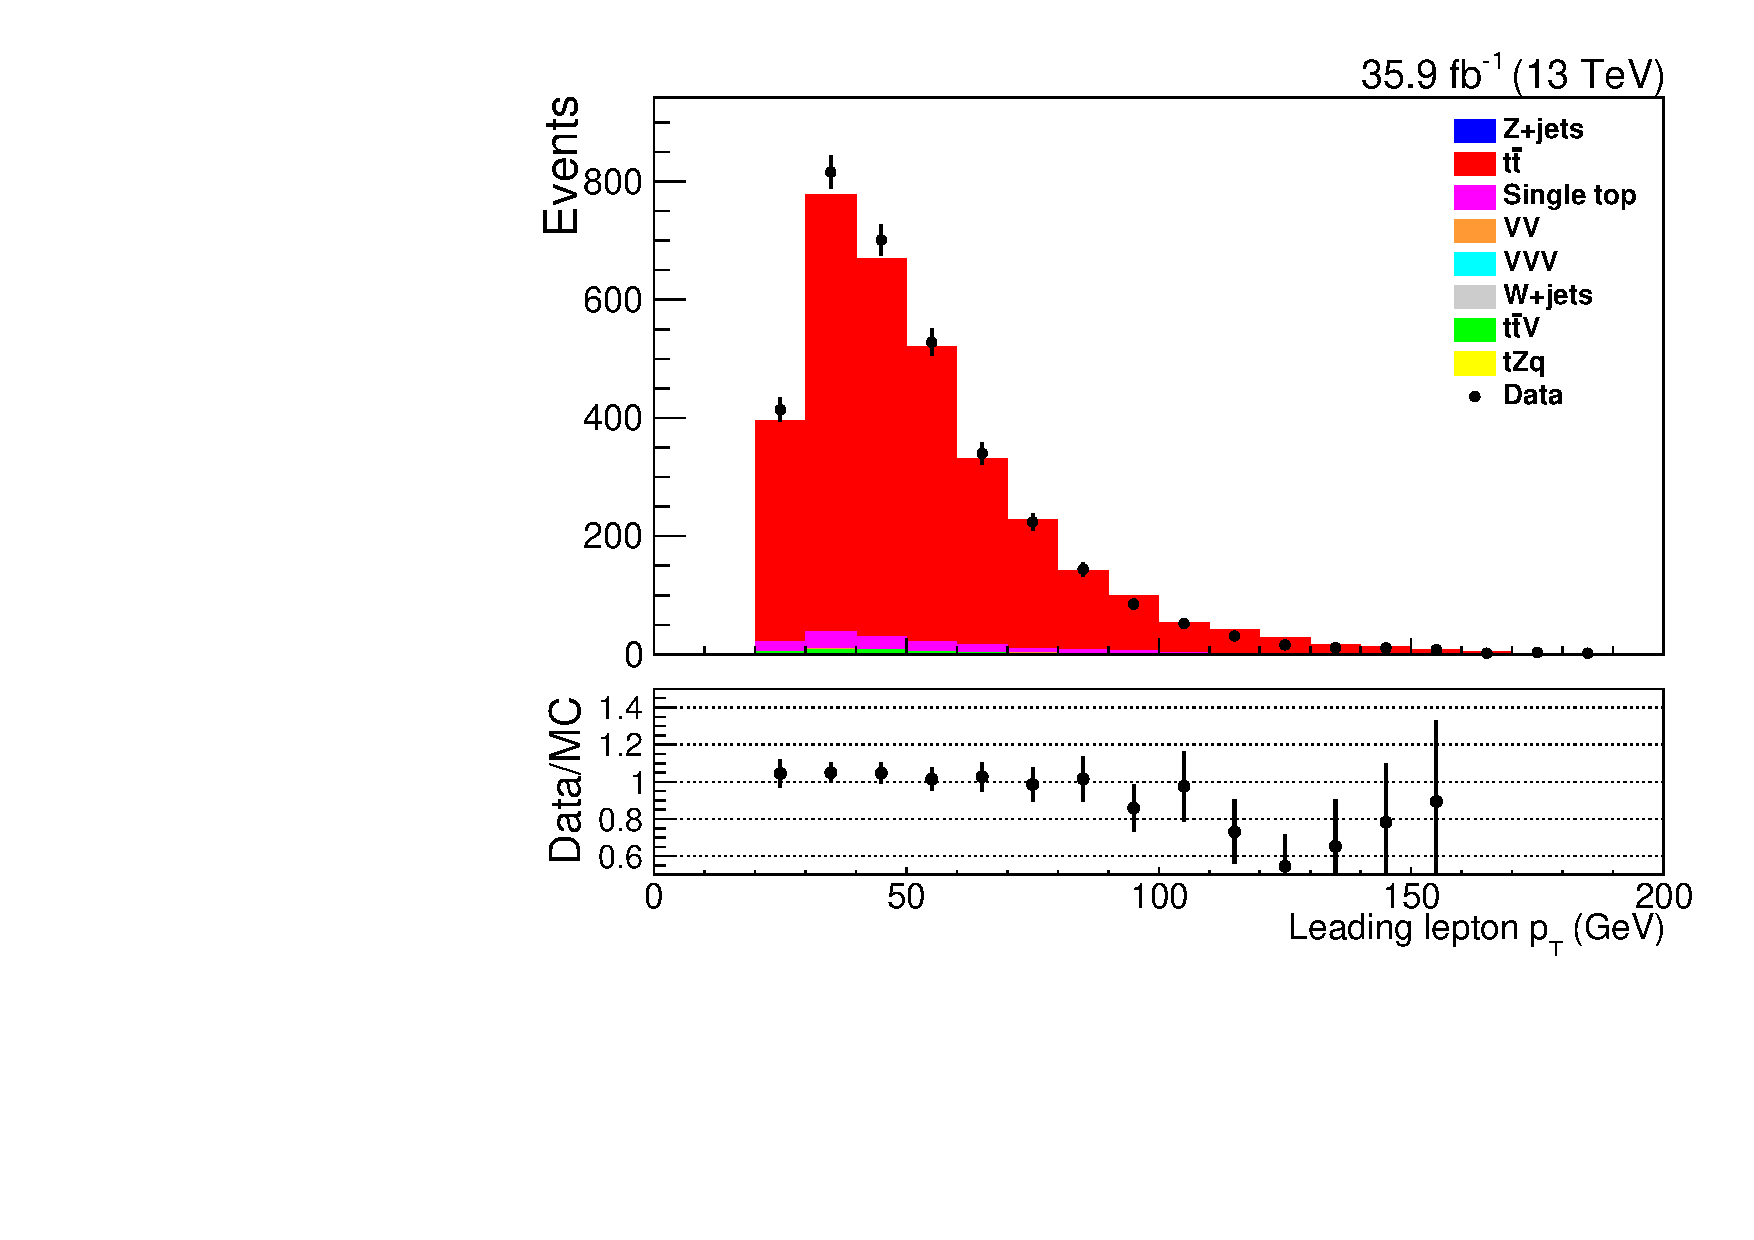
\includegraphics[width=0.47\textwidth]{figs/background-estimation/plots/unblinded/ttbar_control/lep1Pt_SingleTop_wMass_emu.pdf}
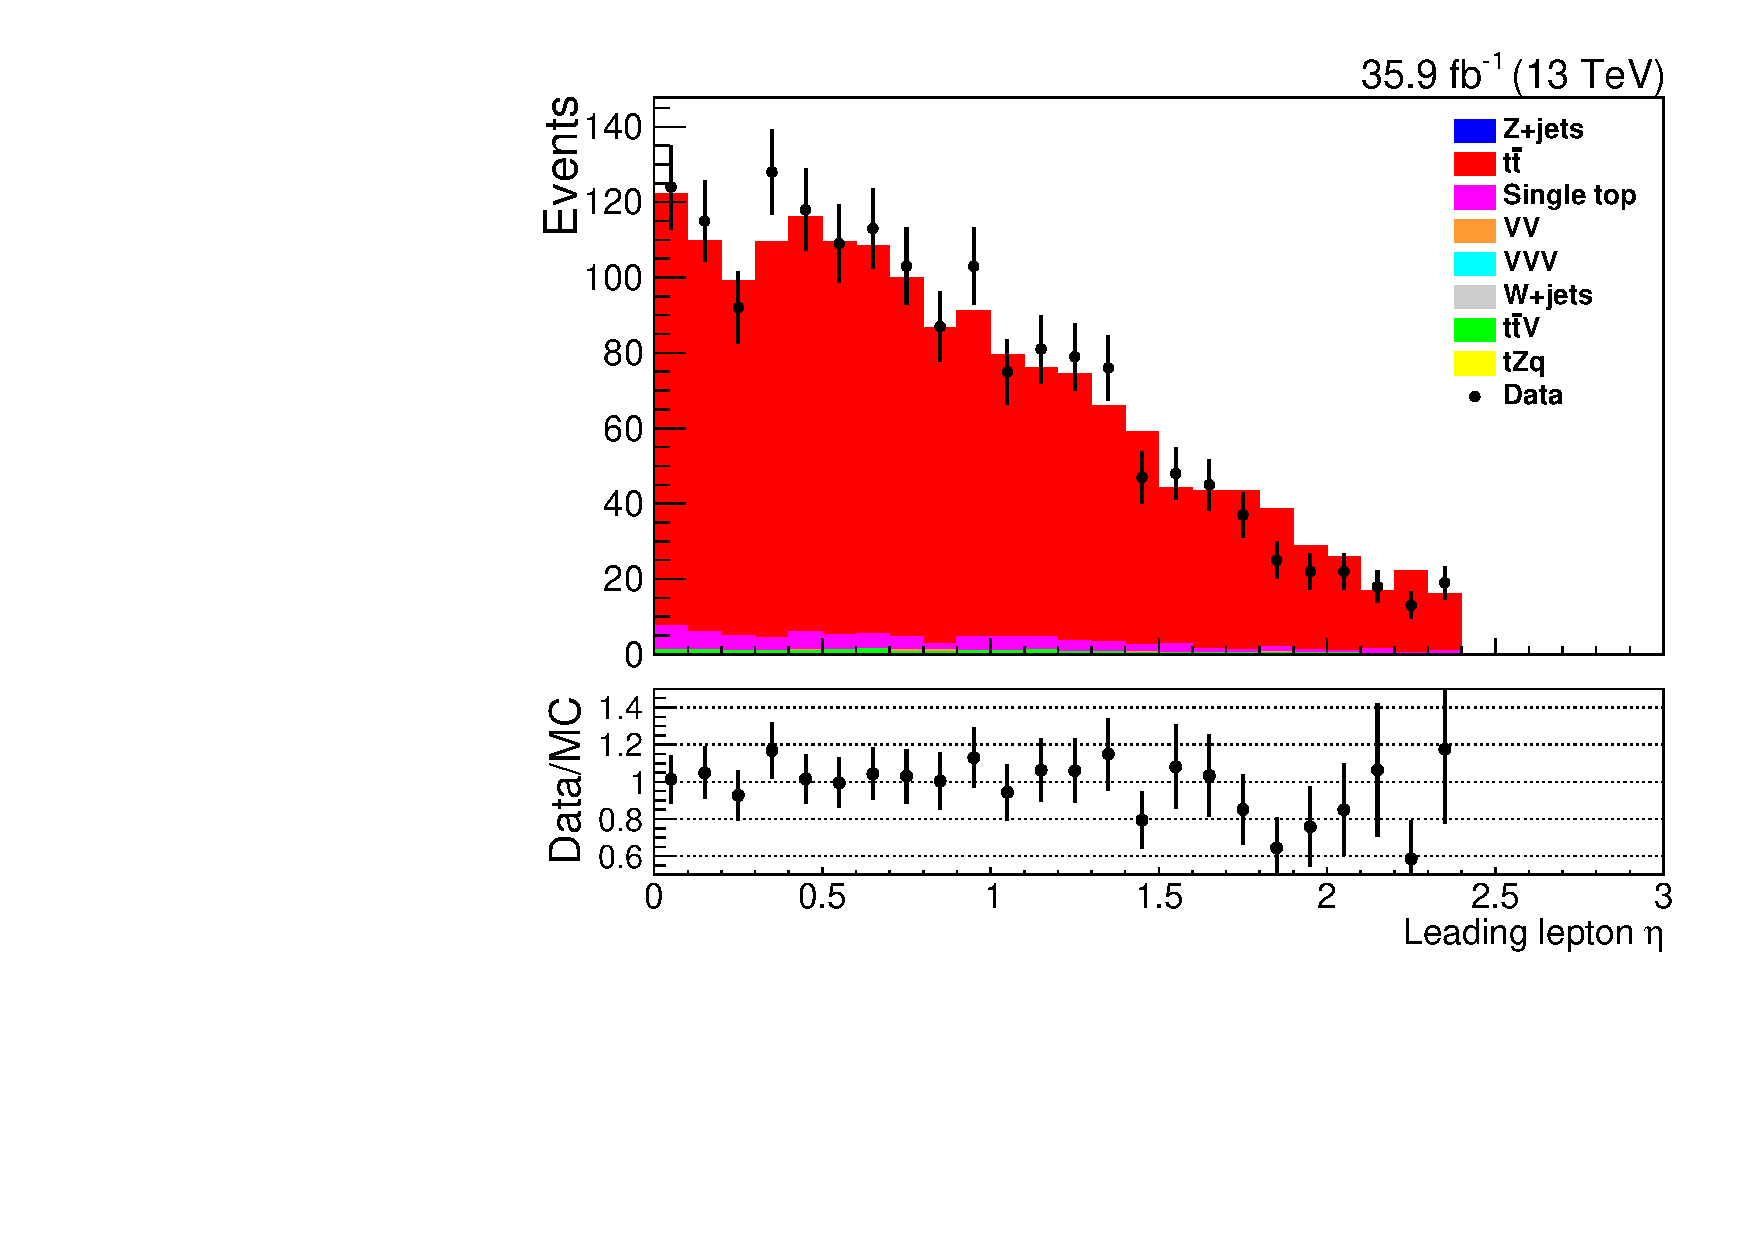
\includegraphics[width=0.47\textwidth]{figs/background-estimation/plots/unblinded/ttbar_control/lep1Eta_SingleTop_wMass_emu.pdf}
\caption{
The electron \pT (left) and $\eta$ (right) following applying the lepton selection criteria (top), the jet selection criteria (middle) and all of the \ttbar control region selection criteria (bottom).
}
\label{fig:ttbar_electron}
\end{figure}

\begin{figure}[h]
\centering
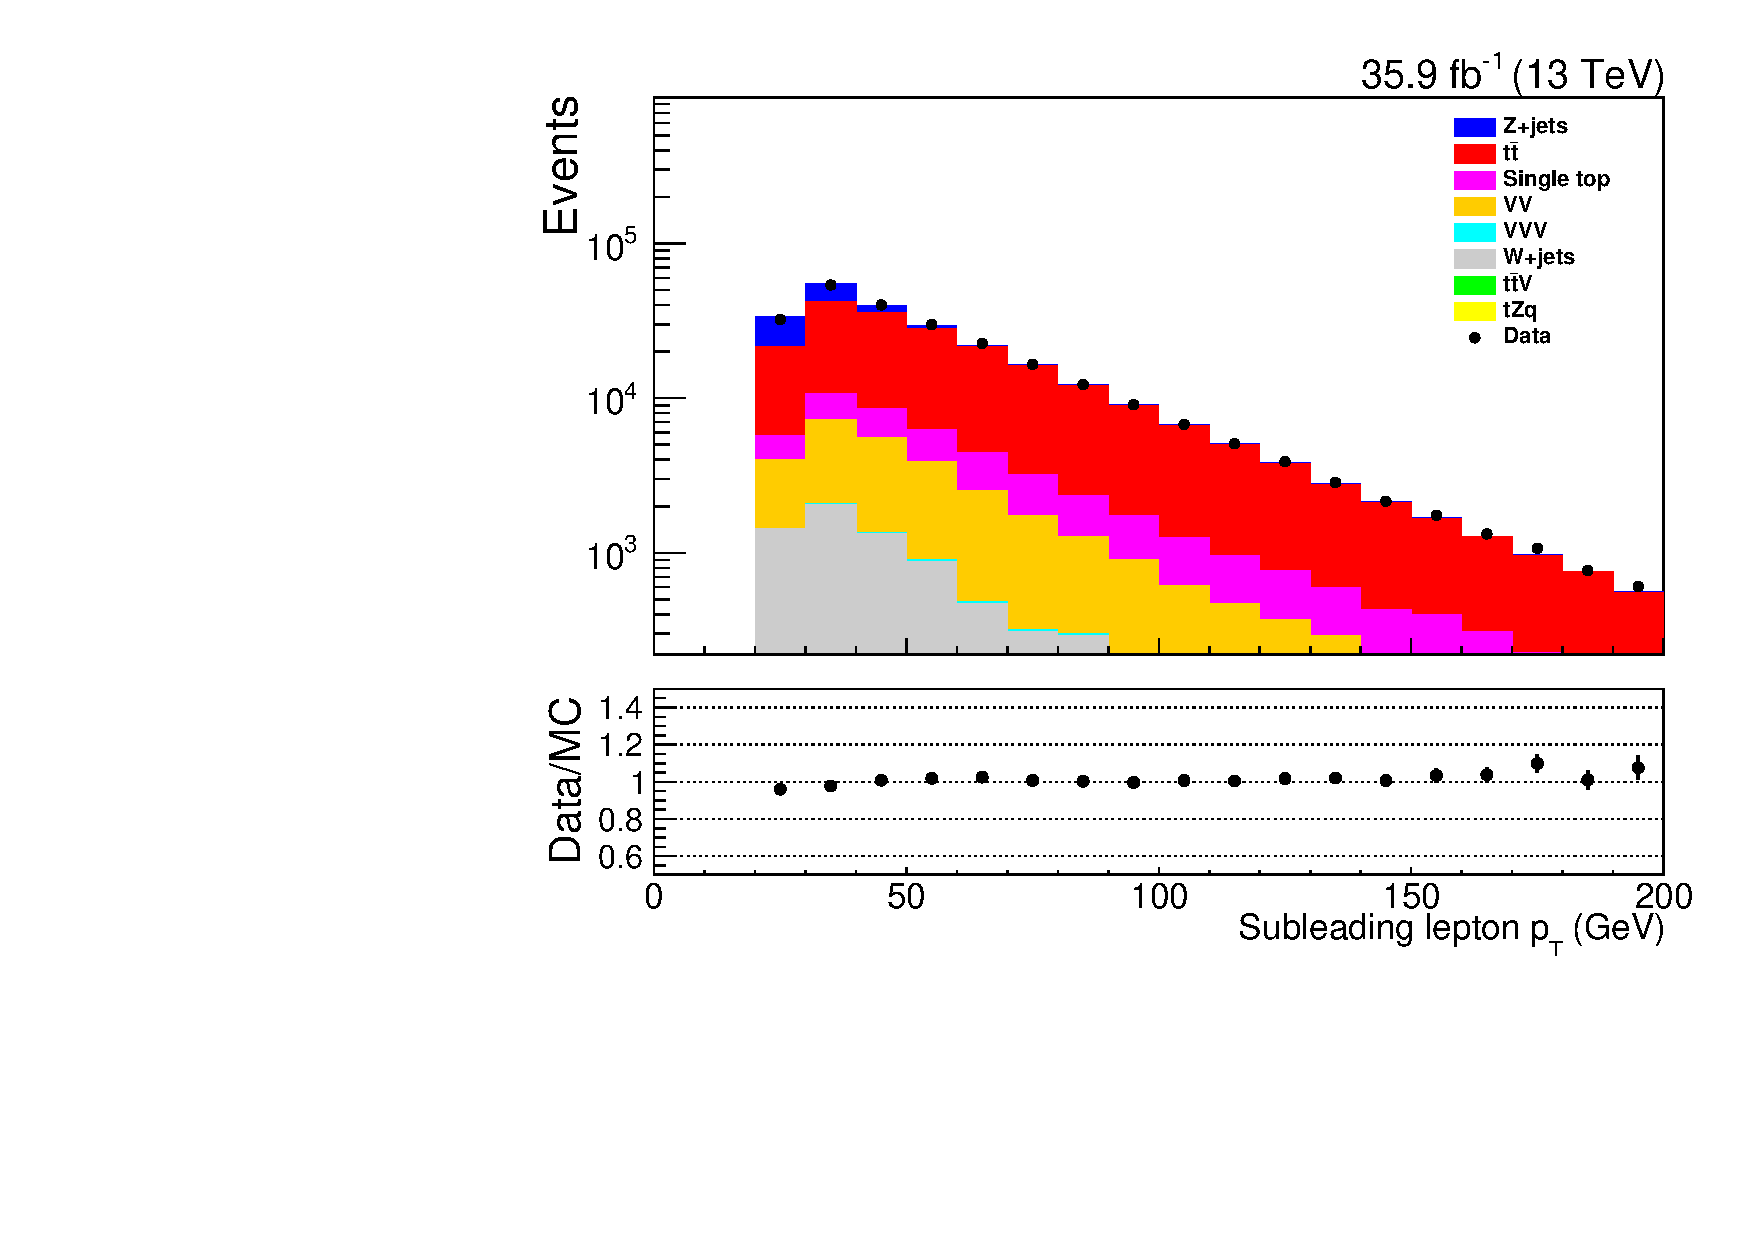
\includegraphics[width=0.47\textwidth]{figs/background-estimation/plots/unblinded/ttbar_control/lep2Pt_SingleTop_lepSel_emu_log.pdf}
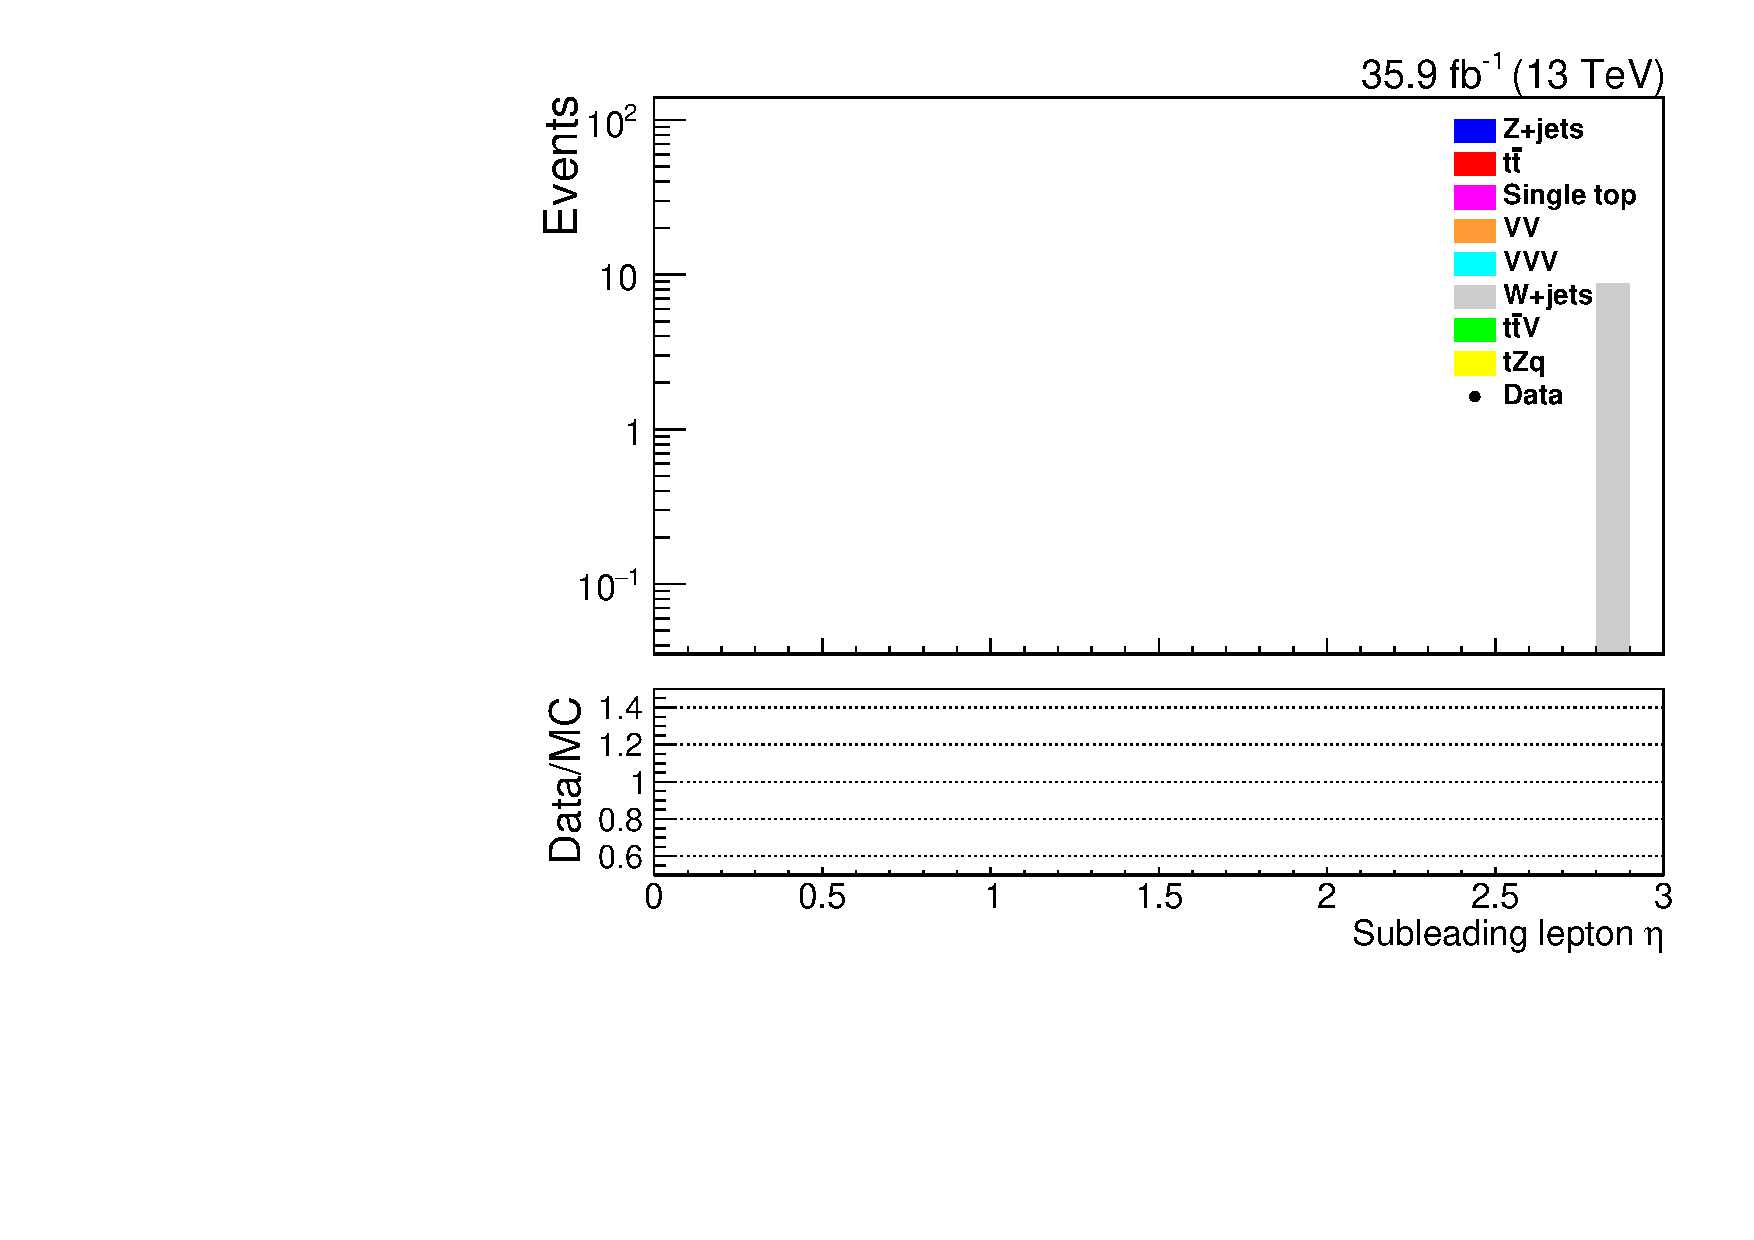
\includegraphics[width=0.47\textwidth]{figs/background-estimation/plots/unblinded/ttbar_control/lep2Eta_SingleTop_lepSel_emu_log.pdf}
\\
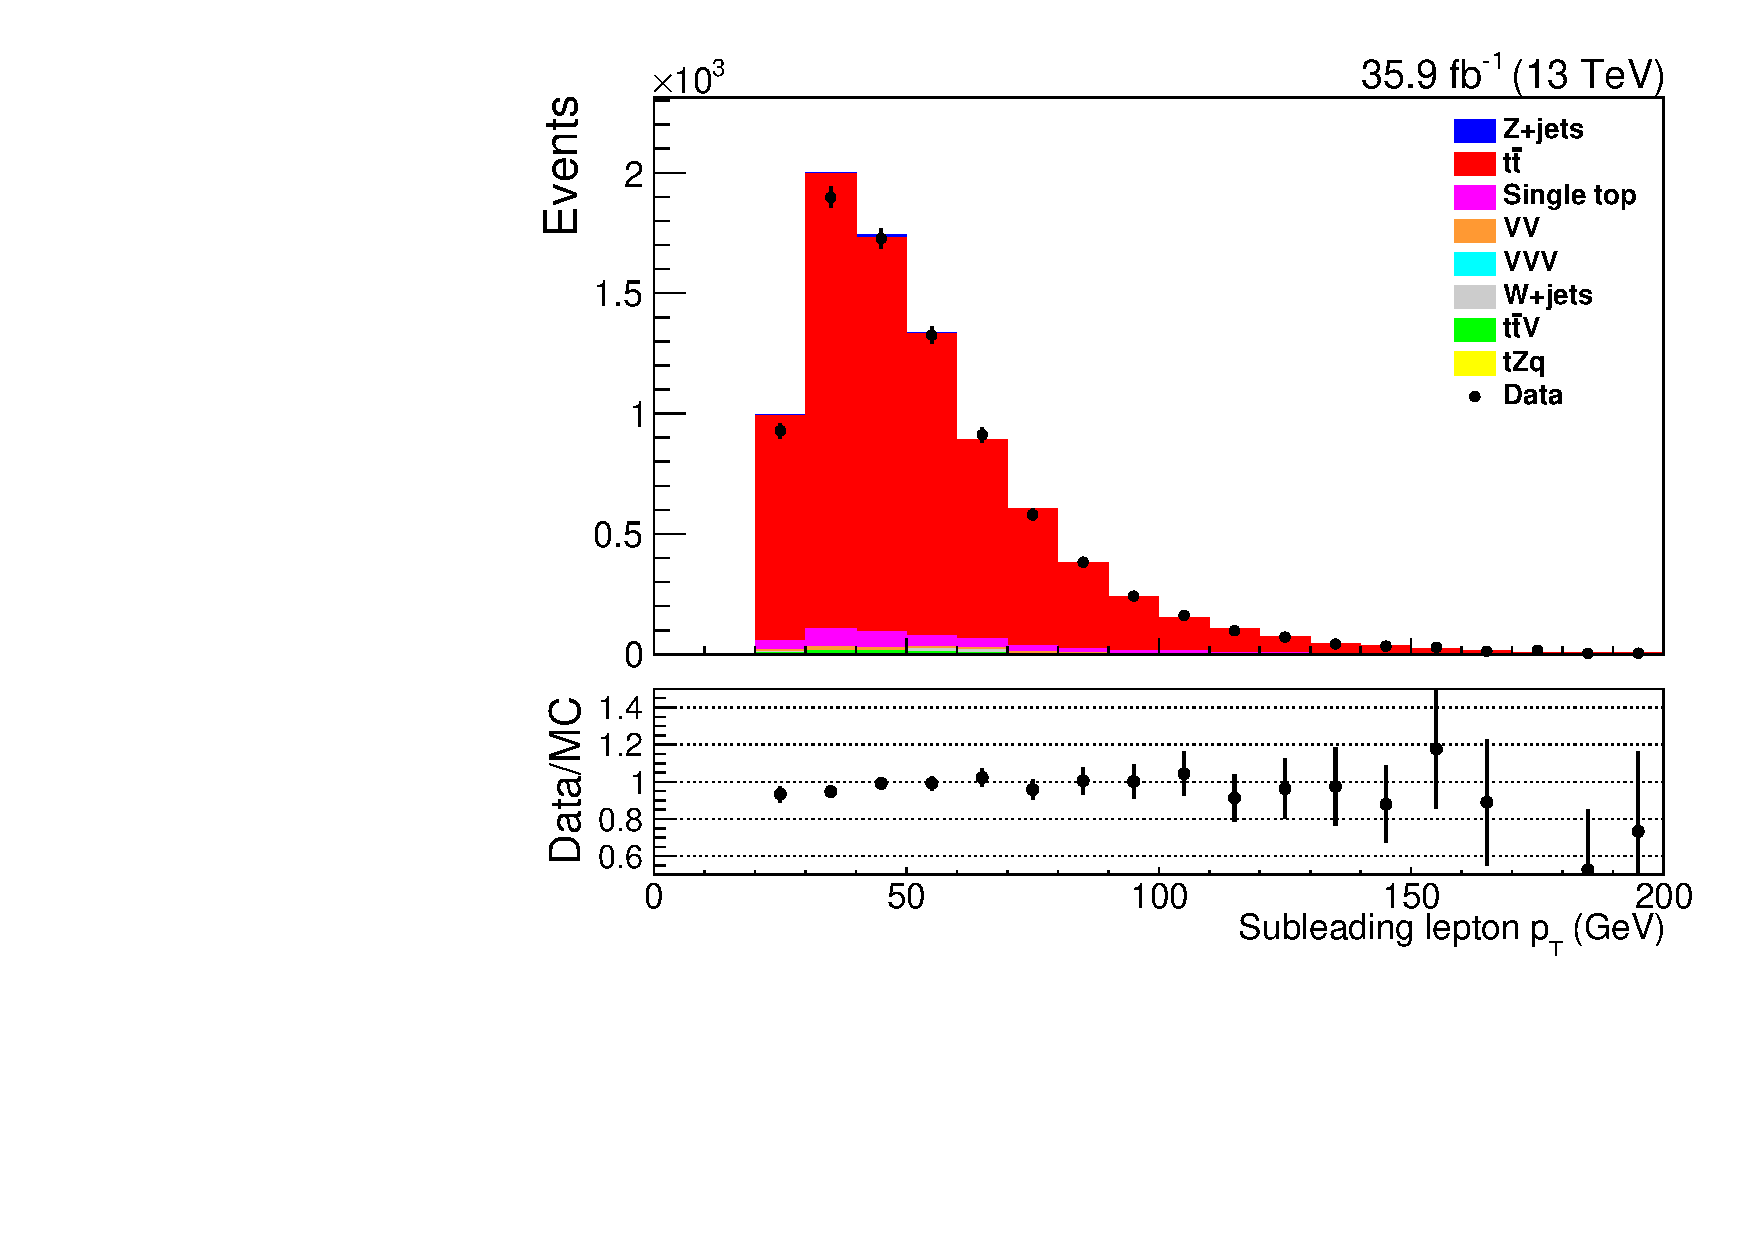
\includegraphics[width=0.47\textwidth]{figs/background-estimation/plots/unblinded/ttbar_control/lep2Pt_SingleTop_jetSel_emu.pdf}
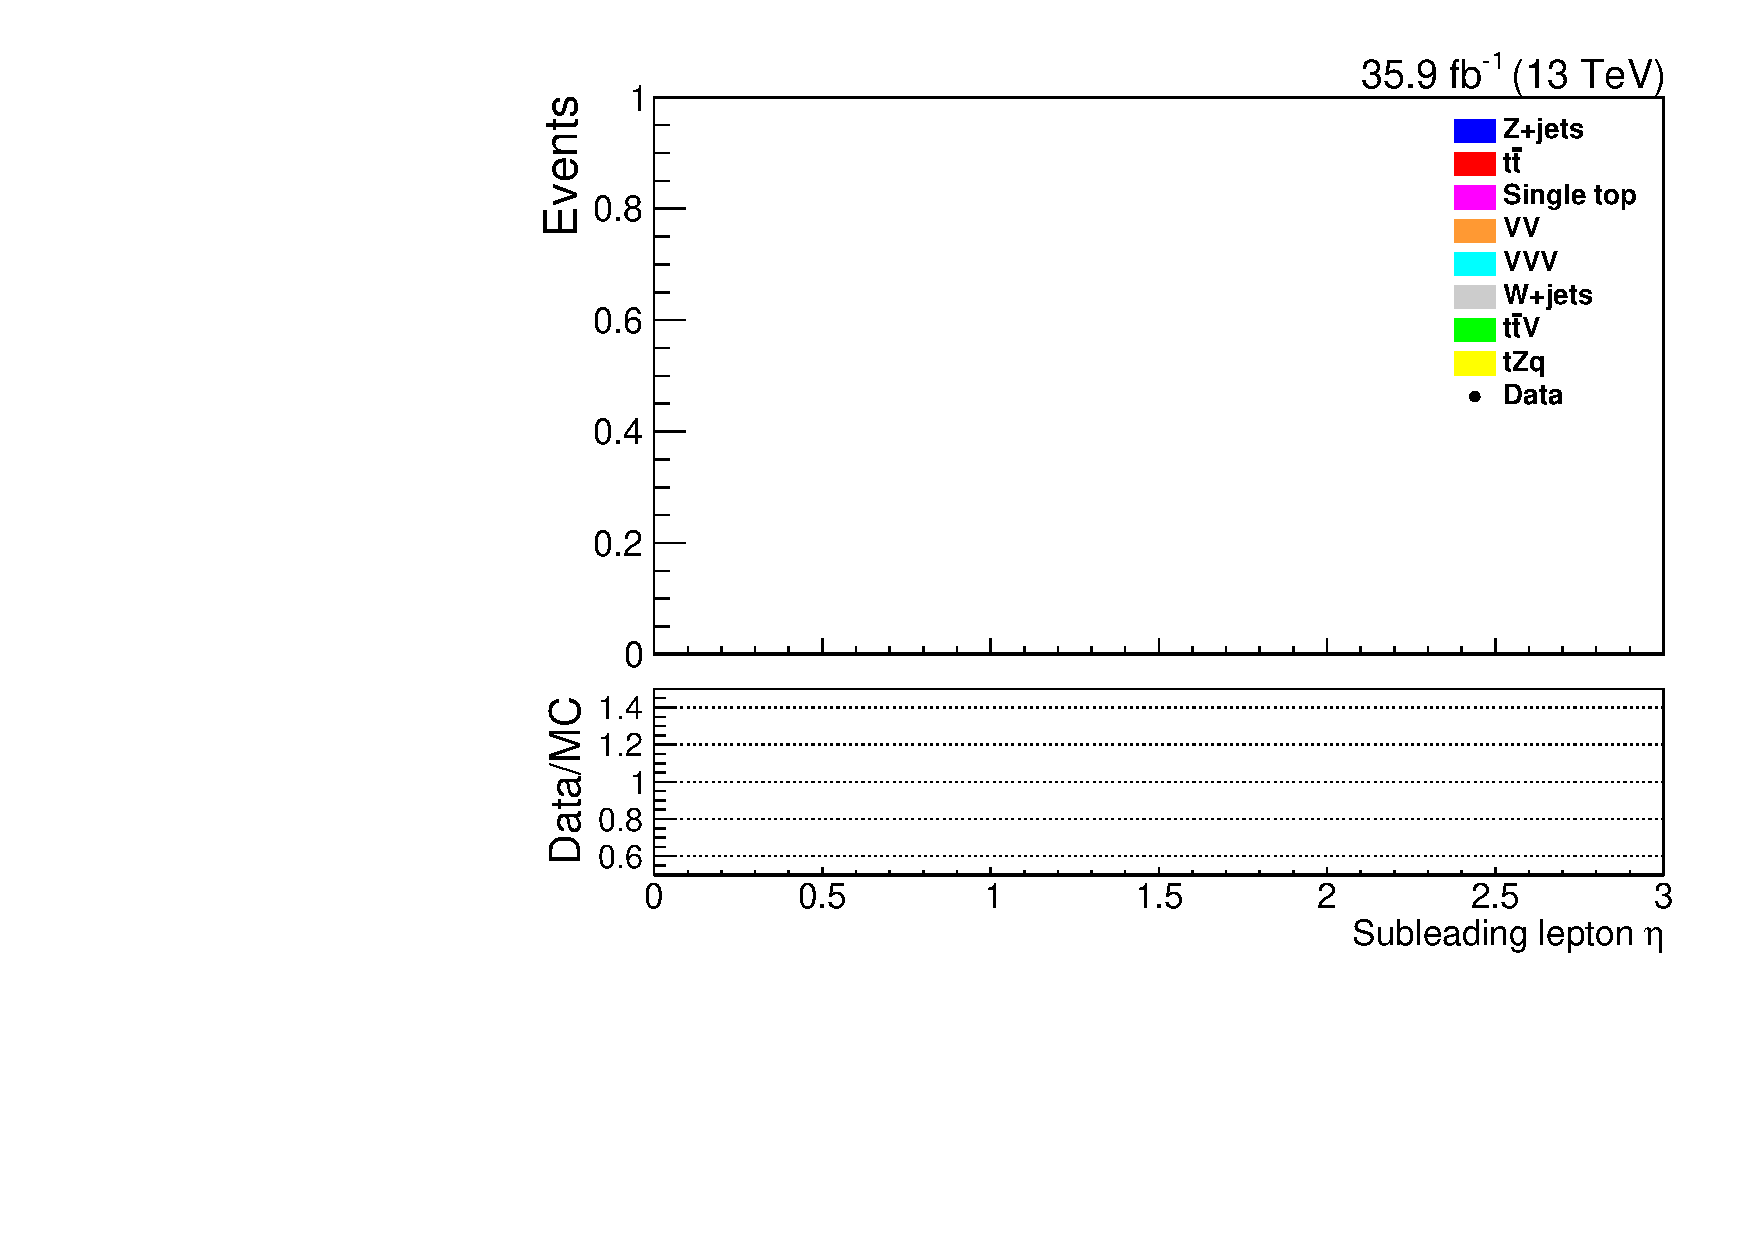
\includegraphics[width=0.47\textwidth]{figs/background-estimation/plots/unblinded/ttbar_control/lep2Eta_SingleTop_jetSel_emu.pdf}
\\
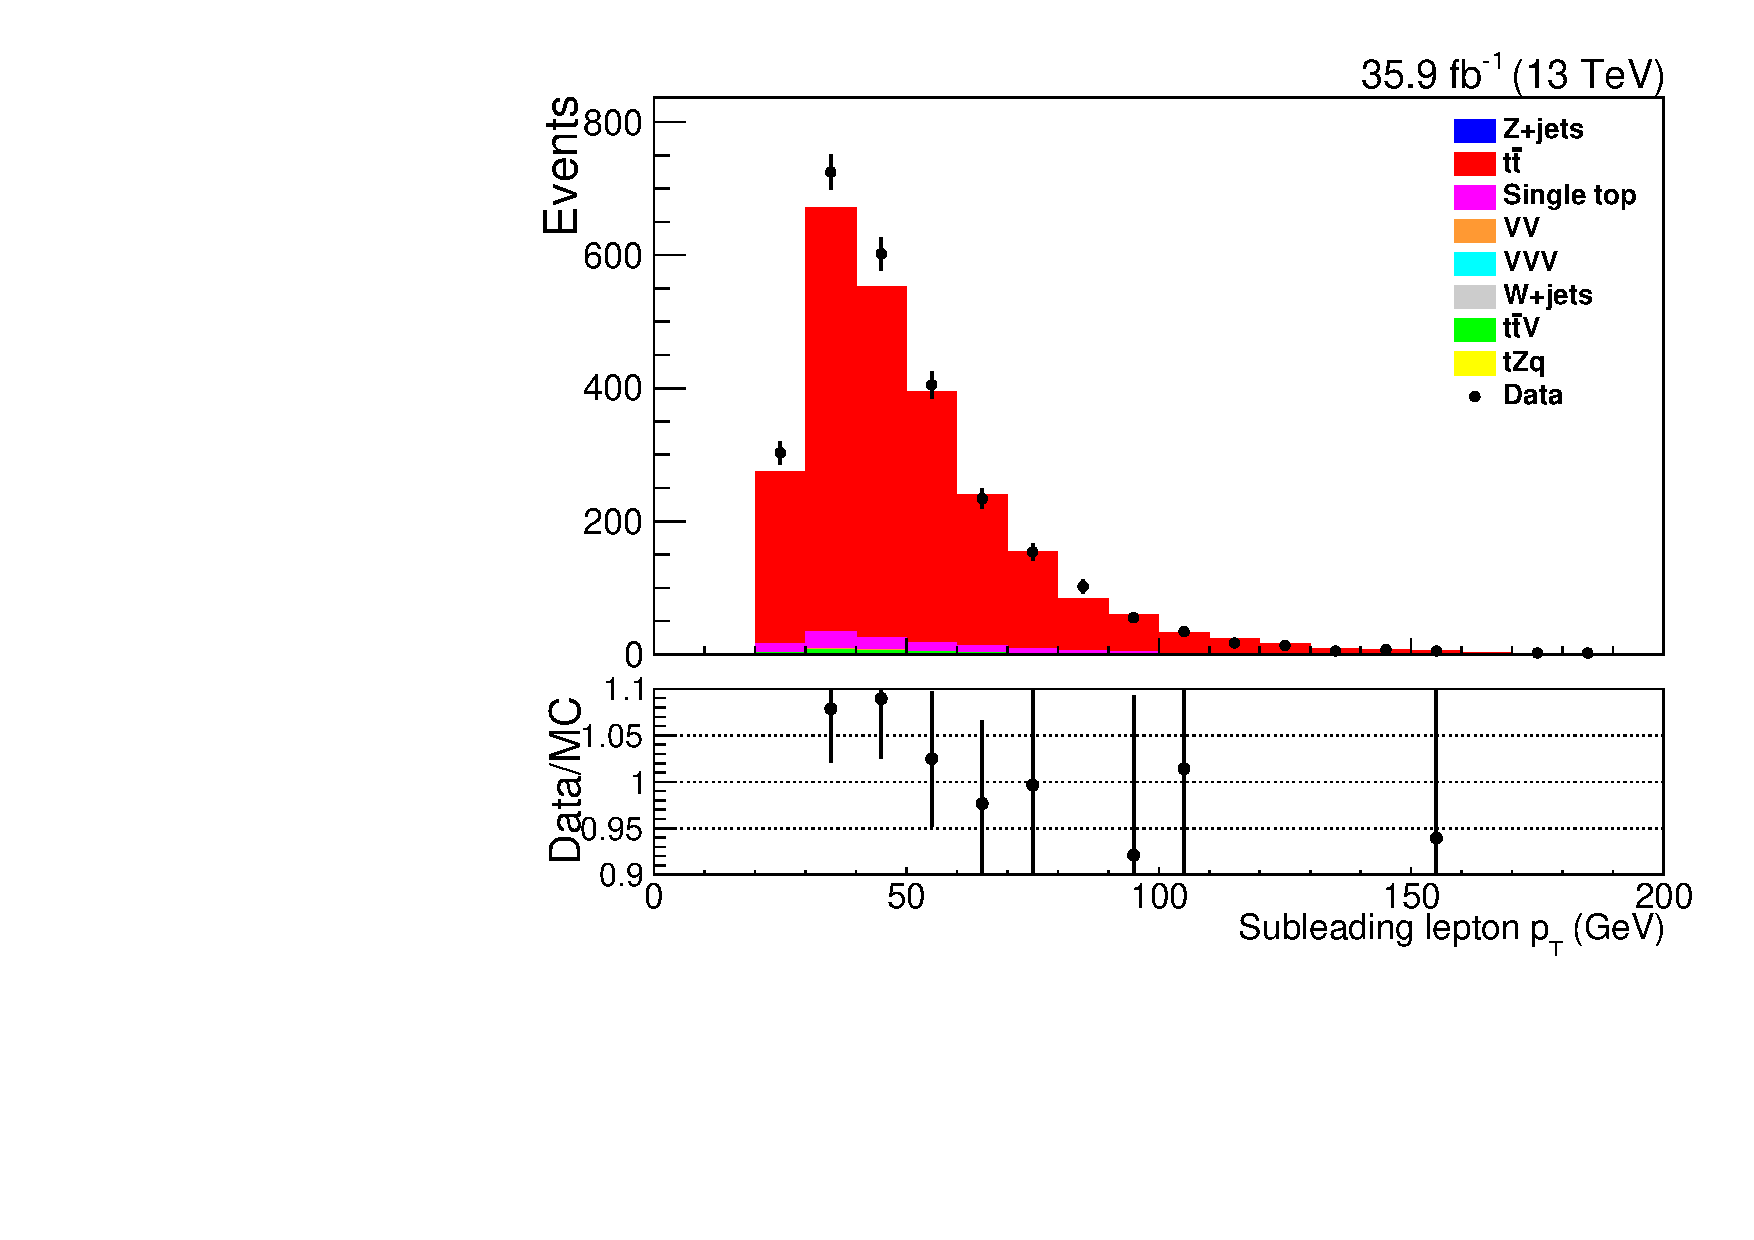
\includegraphics[width=0.47\textwidth]{figs/background-estimation/plots/unblinded/ttbar_control/lep2Pt_SingleTop_wMass_emu.pdf}
\includegraphics[width=0.47\textwidth]{figs/background-estimation/plots/unblinded/ttbar_control/lep2Eta_SingleTop_wMass_emu.pdf}
\caption{
The muon \pT (left) and $\eta$ (right) following applying the lepton selection criteria (top), the jet selection criteria (middle) and all of the \ttbar control region selection criteria (bottom).
}
\label{fig:ttbar_muon}
\end{figure}

\begin{figure}[h]
\centering
\hspace*{-7.3cm}\includegraphics[width=0.47\textwidth]{figs/background-estimation/plots/unblinded/ttbar_control/numbJets_SingleTop_lepSel_emu.pdf}
\\
\includegraphics[width=0.47\textwidth]{figs/background-estimation/plots/unblinded/ttbar_control/numbJets_SingleTop_jetSel_emu.pdf}
\includegraphics[width=0.47\textwidth]{figs/background-estimation/plots/unblinded/ttbar_control/numbBJets_SingleTop_jetSel_emu.pdf}
\\
\includegraphics[width=0.47\textwidth]{figs/background-estimation/plots/unblinded/ttbar_control/numbJets_SingleTop_wMass_emu.pdf}
\includegraphics[width=0.47\textwidth]{figs/background-estimation/plots/unblinded/ttbar_control/numbBJets_SingleTop_wMass_emu.pdf}
\caption{
The number of jets (left) and b-tagged jets (right) following applying the lepton selection criteria (top), the jet selection criteria (middle) and all of the \ttbar control region selection criteria (bottom).
}
\label{fig:ttbar_nJets}
\end{figure}

\begin{figure}[h]
\centering
\includegraphics[width=0.47\textwidth]{figs/background-estimation/plots/unblinded/ttbar_control/leadingJetPt_SingleTop_jetSel_emu.pdf}
\includegraphics[width=0.47\textwidth]{figs/background-estimation/plots/unblinded/ttbar_control/leadingJetEta_SingleTop_jetSel_emu.pdf}
\\
\includegraphics[width=0.47\textwidth]{figs/background-estimation/plots/unblinded/ttbar_control/secondJetPt_SingleTop_jetSel_emu.pdf}
\includegraphics[width=0.47\textwidth]{figs/background-estimation/plots/unblinded/ttbar_control/secondJetEta_SingleTop_jetSel_emu.pdf}
\\
\includegraphics[width=0.47\textwidth]{figs/background-estimation/plots/unblinded/ttbar_control/thirdJetPt_SingleTop_jetSel_emu.pdf}
\includegraphics[width=0.47\textwidth]{figs/background-estimation/plots/unblinded/ttbar_control/thirdJetEta_SingleTop_jetSel_emu.pdf}
\\
\includegraphics[width=0.47\textwidth]{figs/background-estimation/plots/unblinded/ttbar_control/fourthJetPt_SingleTop_jetSel_emu.pdf}
\includegraphics[width=0.47\textwidth]{figs/background-estimation/plots/unblinded/ttbar_control/fourthJetEta_SingleTop_jetSel_emu.pdf}
\caption{
The \pT (left) and $\eta$ (right) of the leading (top), sub-leading (upper middle), third (lower middle) and fourth (bottom) jets following the application of the jet selection criteria.
}
\label{fig:ttbar_jetsKinematics_jetCuts}
\end{figure}

\begin{figure}[h]
\centering
\includegraphics[width=0.47\textwidth]{figs/background-estimation/plots/unblinded/ttbar_control/leadingJetPt_SingleTop_wMass_emu.pdf}
\includegraphics[width=0.47\textwidth]{figs/background-estimation/plots/unblinded/ttbar_control/leadingJetEta_SingleTop_wMass_emu.pdf}
\\
\includegraphics[width=0.47\textwidth]{figs/background-estimation/plots/unblinded/ttbar_control/secondJetPt_SingleTop_wMass_emu.pdf}
\includegraphics[width=0.47\textwidth]{figs/background-estimation/plots/unblinded/ttbar_control/secondJetEta_SingleTop_wMass_emu.pdf}
\\
\includegraphics[width=0.47\textwidth]{figs/background-estimation/plots/unblinded/ttbar_control/thirdJetPt_SingleTop_wMass_emu.pdf}
\includegraphics[width=0.47\textwidth]{figs/background-estimation/plots/unblinded/ttbar_control/thirdJetEta_SingleTop_wMass_emu.pdf}
\\
\includegraphics[width=0.47\textwidth]{figs/background-estimation/plots/unblinded/ttbar_control/fourthJetPt_SingleTop_wMass_emu.pdf}
\includegraphics[width=0.47\textwidth]{figs/background-estimation/plots/unblinded/ttbar_control/fourthJetEta_SingleTop_wMass_emu.pdf}
\caption{
The \pT (left) and $\eta$ (right) of the leading (top), sub-leading (upper middle), third (lower middle) and fourth (bottom) jets following the application of all of the \ttbar control region selection criteria.
}
\label{fig:ttbar_jetsKinematics_wMass}
\end{figure}